% Options for packages loaded elsewhere
\PassOptionsToPackage{unicode}{hyperref}
\PassOptionsToPackage{hyphens}{url}
%
\documentclass[
]{book}
\usepackage{amsmath,amssymb}
\usepackage{lmodern}
\usepackage{ifxetex,ifluatex}
\ifnum 0\ifxetex 1\fi\ifluatex 1\fi=0 % if pdftex
  \usepackage[T1]{fontenc}
  \usepackage[utf8]{inputenc}
  \usepackage{textcomp} % provide euro and other symbols
\else % if luatex or xetex
  \usepackage{unicode-math}
  \defaultfontfeatures{Scale=MatchLowercase}
  \defaultfontfeatures[\rmfamily]{Ligatures=TeX,Scale=1}
\fi
% Use upquote if available, for straight quotes in verbatim environments
\IfFileExists{upquote.sty}{\usepackage{upquote}}{}
\IfFileExists{microtype.sty}{% use microtype if available
  \usepackage[]{microtype}
  \UseMicrotypeSet[protrusion]{basicmath} % disable protrusion for tt fonts
}{}
\makeatletter
\@ifundefined{KOMAClassName}{% if non-KOMA class
  \IfFileExists{parskip.sty}{%
    \usepackage{parskip}
  }{% else
    \setlength{\parindent}{0pt}
    \setlength{\parskip}{6pt plus 2pt minus 1pt}}
}{% if KOMA class
  \KOMAoptions{parskip=half}}
\makeatother
\usepackage{xcolor}
\IfFileExists{xurl.sty}{\usepackage{xurl}}{} % add URL line breaks if available
\IfFileExists{bookmark.sty}{\usepackage{bookmark}}{\usepackage{hyperref}}
\hypersetup{
  pdftitle={Meta Analysis of cross-sectional studies},
  pdfauthor={Benoit Bediou},
  hidelinks,
  pdfcreator={LaTeX via pandoc}}
\urlstyle{same} % disable monospaced font for URLs
\usepackage{color}
\usepackage{fancyvrb}
\newcommand{\VerbBar}{|}
\newcommand{\VERB}{\Verb[commandchars=\\\{\}]}
\DefineVerbatimEnvironment{Highlighting}{Verbatim}{commandchars=\\\{\}}
% Add ',fontsize=\small' for more characters per line
\usepackage{framed}
\definecolor{shadecolor}{RGB}{248,248,248}
\newenvironment{Shaded}{\begin{snugshade}}{\end{snugshade}}
\newcommand{\AlertTok}[1]{\textcolor[rgb]{0.94,0.16,0.16}{#1}}
\newcommand{\AnnotationTok}[1]{\textcolor[rgb]{0.56,0.35,0.01}{\textbf{\textit{#1}}}}
\newcommand{\AttributeTok}[1]{\textcolor[rgb]{0.77,0.63,0.00}{#1}}
\newcommand{\BaseNTok}[1]{\textcolor[rgb]{0.00,0.00,0.81}{#1}}
\newcommand{\BuiltInTok}[1]{#1}
\newcommand{\CharTok}[1]{\textcolor[rgb]{0.31,0.60,0.02}{#1}}
\newcommand{\CommentTok}[1]{\textcolor[rgb]{0.56,0.35,0.01}{\textit{#1}}}
\newcommand{\CommentVarTok}[1]{\textcolor[rgb]{0.56,0.35,0.01}{\textbf{\textit{#1}}}}
\newcommand{\ConstantTok}[1]{\textcolor[rgb]{0.00,0.00,0.00}{#1}}
\newcommand{\ControlFlowTok}[1]{\textcolor[rgb]{0.13,0.29,0.53}{\textbf{#1}}}
\newcommand{\DataTypeTok}[1]{\textcolor[rgb]{0.13,0.29,0.53}{#1}}
\newcommand{\DecValTok}[1]{\textcolor[rgb]{0.00,0.00,0.81}{#1}}
\newcommand{\DocumentationTok}[1]{\textcolor[rgb]{0.56,0.35,0.01}{\textbf{\textit{#1}}}}
\newcommand{\ErrorTok}[1]{\textcolor[rgb]{0.64,0.00,0.00}{\textbf{#1}}}
\newcommand{\ExtensionTok}[1]{#1}
\newcommand{\FloatTok}[1]{\textcolor[rgb]{0.00,0.00,0.81}{#1}}
\newcommand{\FunctionTok}[1]{\textcolor[rgb]{0.00,0.00,0.00}{#1}}
\newcommand{\ImportTok}[1]{#1}
\newcommand{\InformationTok}[1]{\textcolor[rgb]{0.56,0.35,0.01}{\textbf{\textit{#1}}}}
\newcommand{\KeywordTok}[1]{\textcolor[rgb]{0.13,0.29,0.53}{\textbf{#1}}}
\newcommand{\NormalTok}[1]{#1}
\newcommand{\OperatorTok}[1]{\textcolor[rgb]{0.81,0.36,0.00}{\textbf{#1}}}
\newcommand{\OtherTok}[1]{\textcolor[rgb]{0.56,0.35,0.01}{#1}}
\newcommand{\PreprocessorTok}[1]{\textcolor[rgb]{0.56,0.35,0.01}{\textit{#1}}}
\newcommand{\RegionMarkerTok}[1]{#1}
\newcommand{\SpecialCharTok}[1]{\textcolor[rgb]{0.00,0.00,0.00}{#1}}
\newcommand{\SpecialStringTok}[1]{\textcolor[rgb]{0.31,0.60,0.02}{#1}}
\newcommand{\StringTok}[1]{\textcolor[rgb]{0.31,0.60,0.02}{#1}}
\newcommand{\VariableTok}[1]{\textcolor[rgb]{0.00,0.00,0.00}{#1}}
\newcommand{\VerbatimStringTok}[1]{\textcolor[rgb]{0.31,0.60,0.02}{#1}}
\newcommand{\WarningTok}[1]{\textcolor[rgb]{0.56,0.35,0.01}{\textbf{\textit{#1}}}}
\usepackage{longtable,booktabs,array}
\usepackage{calc} % for calculating minipage widths
% Correct order of tables after \paragraph or \subparagraph
\usepackage{etoolbox}
\makeatletter
\patchcmd\longtable{\par}{\if@noskipsec\mbox{}\fi\par}{}{}
\makeatother
% Allow footnotes in longtable head/foot
\IfFileExists{footnotehyper.sty}{\usepackage{footnotehyper}}{\usepackage{footnote}}
\makesavenoteenv{longtable}
\usepackage{graphicx}
\makeatletter
\def\maxwidth{\ifdim\Gin@nat@width>\linewidth\linewidth\else\Gin@nat@width\fi}
\def\maxheight{\ifdim\Gin@nat@height>\textheight\textheight\else\Gin@nat@height\fi}
\makeatother
% Scale images if necessary, so that they will not overflow the page
% margins by default, and it is still possible to overwrite the defaults
% using explicit options in \includegraphics[width, height, ...]{}
\setkeys{Gin}{width=\maxwidth,height=\maxheight,keepaspectratio}
% Set default figure placement to htbp
\makeatletter
\def\fps@figure{htbp}
\makeatother
\setlength{\emergencystretch}{3em} % prevent overfull lines
\providecommand{\tightlist}{%
  \setlength{\itemsep}{0pt}\setlength{\parskip}{0pt}}
\setcounter{secnumdepth}{5}
\usepackage{booktabs}
\usepackage{booktabs}
\usepackage{longtable}
\usepackage{array}
\usepackage{multirow}
\usepackage{wrapfig}
\usepackage{float}
\usepackage{colortbl}
\usepackage{pdflscape}
\usepackage{tabu}
\usepackage{threeparttable}
\usepackage{threeparttablex}
\usepackage[normalem]{ulem}
\usepackage{makecell}
\usepackage{xcolor}
\ifluatex
  \usepackage{selnolig}  % disable illegal ligatures
\fi
\usepackage[]{natbib}
\bibliographystyle{apalike}

\title{Meta Analysis of cross-sectional studies}
\author{Benoit Bediou}
\date{2021-08-04}

\begin{document}
\maketitle

{
\setcounter{tocdepth}{1}
\tableofcontents
}
\hypertarget{preamble}{%
\chapter{Preamble}\label{preamble}}

OSF project: \url{https://osf.io/3xdh8/}

pre-registration: \url{https://osf.io/6qpye}

\hypertarget{intro}{%
\chapter{Introduction}\label{intro}}

Preregistration details and links available in section preamble\ref{preamble}.

This meta-analysis covers 2000-2020. It thus extends partially with the meta-analysis
by Bediou et al.~2018 and extends it by 5 years.

\hypertarget{overview-of-our-first-meta-analysis-bediou-et-al.-2018}{%
\section{Overview of our first meta-analysis (Bediou et al., 2018)}\label{overview-of-our-first-meta-analysis-bediou-et-al.-2018}}

The literature review from our former meta-analysis (Bediou et al., 2018) covered the period between
January 2000 and December 2015. A total of 5,770 abstracts were identified, from which 630 full texts
were thus dimmed eligible. Only 82 manuscripts passed our inclusion/exclusion criteria, comprising
65 published and 17 unpublished studies.\\
The cross-sectional meta-analysis by Bediou et al.~(2018) included 194 effects extracted
from 89 experiments drawn from 73 distinct manuscripts.

\hypertarget{the-present-dataset}{%
\section{The present dataset}\label{the-present-dataset}}

For the present meta-analysis, the search keywords were identical. However, our selection criteria were
slightly different which could result in differences in terms of inclusion or exclusion. Therefore,
all 5,770 abstracts that had been identified by our initial search were re-assessed again for eligibility
by three independent reviewers.
In addition, a new literature search was conducted covering the period January 2015 - June 2020. With this
new search an additional 2,225 abstracts were identified (after removal of duplicates).

With the two searches combined, our selection process started from 3,497 titles, which were reduced to 749 abstracts,
and went further down to 243 full texts.

The table below indicates the number of studies, effects and min/max/median number of effect sizes extracted per study.

\begin{table}
\centering
\begin{tabular}{r|r|r|r|r|r|r}
\hline
studies & effects & es\_min & es\_max & es\_median & es\_Q1 & es\_q3\\
\hline
77 & 467 & 1 & 29 & 4 & 2 & 8\\
\hline
\end{tabular}
\end{table}

Studies with unbalanced gender ratios were discarded from analysis.

In the next section, Chapter \ref{datachecks}, we first review the raw dataset, and then the filtered dataset which was used for all analyses.\\
The final dataset includes \textbf{228 effect sizes extracted from 105 studies found in 73 manuscripts (??X published??)}

\hypertarget{datachecks}{%
\chapter{Data preparation and cleaning}\label{datachecks}}

\hypertarget{rawdata}{%
\section{Raw dataset}\label{rawdata}}

\textbf{included studies}

Our thorough literature review identified potentially relevant studies based on predefined keywords.\\
After screening of eligible studies, the \emph{raw} data set includes:\\
- 77 manuscripts\\
- 112 studies\\
- 97 independent samples of participants

\emph{\# effect sizes per paper}

\begin{table}
\centering
\begin{tabular}{r|r|r|r|r|r|r}
\hline
manuscripts & effects & es\_min & es\_max & es\_median & es\_Q1 & es\_Q3\\
\hline
77 & 467 & 1 & 29 & 4 & 2 & 8\\
\hline
\end{tabular}
\end{table}

Second, we checked gender distributions of the AVGP and NVGP groups.

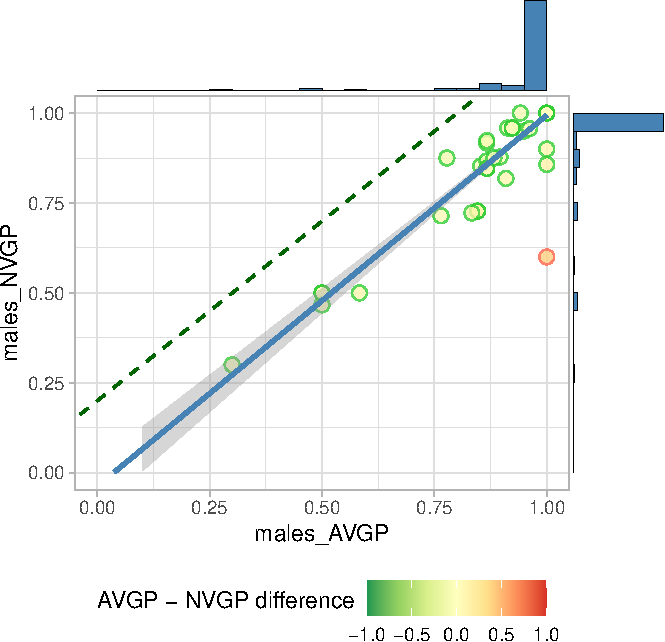
\includegraphics{MetaAnalysis_CrossSectional_files/figure-latex/genderDistrib-1.pdf}

There is a predominance of males in both AVGPs and NVGPs.
The green and orange dashed lines define 3 regions on the between-group difference
in the proportion of males:\\
- The upper left region (above green) contains studies with greater proportion of males in NVGPs\\
- The bottom right corner (below orange) contains studies with more males in AVGPs\\
- Between these two lines are studies with less than 25\% difference in gender ratio

There is a bias toward having more males in the AVGP group.\\
Therefore, only studies with a difference in gender ratio less than 25\%
will be included in subsequent plots and analyses

These studies are shown with a green contour

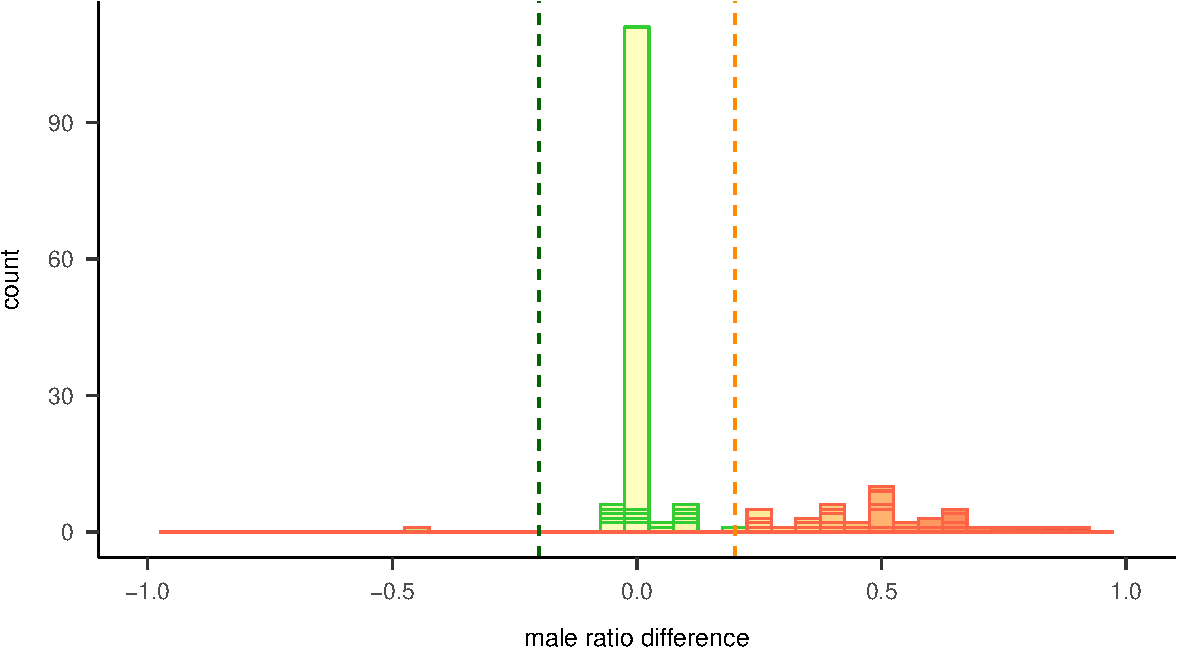
\includegraphics{MetaAnalysis_CrossSectional_files/figure-latex/genderPlot-1.pdf}

When the difference exceeded 20\%, authors were contacted in order to obtain data
from male-only samples, only if a minimum of 10 participants in each group.

\textbf{excluded studies}

Studies excluded at the data extraction stage for various reasons: gender imbalance, criteria for defining AVGP or NVGPs, etc.\\
\emph{\# effect sizes per paper - excluded studies only}

\begin{table}
\centering
\begin{tabular}{r|r}
\hline
studies & effects\\
\hline
35 & 60\\
\hline
\end{tabular}
\end{table}

\hypertarget{cleandata}{%
\section{Filtered dataset (i.e., matched gender)}\label{cleandata}}

Effect sizes as well subject and study characteristics were then extracted from all studies that were eligible.

After exclusion of studies with unbalanced gender, the final data set includes:\\
- 230 effect sizes\\
- 74 papers\\
- 106 studies\\
- 91 independent samples

\begin{Shaded}
\begin{Highlighting}[]
\NormalTok{es\_data }\SpecialCharTok{\%\textgreater{}\%}
  \FunctionTok{group\_by}\NormalTok{(Paper) }\SpecialCharTok{\%\textgreater{}\%}
  \FunctionTok{summarise}\NormalTok{(}\AttributeTok{es =} \FunctionTok{n}\NormalTok{()) }\SpecialCharTok{\%\textgreater{}\%}
  \FunctionTok{summarise}\NormalTok{(}
    \AttributeTok{manuscripts =} \FunctionTok{n}\NormalTok{(), }
    \AttributeTok{effects =} \FunctionTok{sum}\NormalTok{(es),}
    \AttributeTok{es\_min =} \FunctionTok{min}\NormalTok{(es),}
    \AttributeTok{es\_max =} \FunctionTok{max}\NormalTok{(es),}
    \AttributeTok{es\_median =} \FunctionTok{median}\NormalTok{(es),}
    \AttributeTok{es\_Q1 =} \FunctionTok{quantile}\NormalTok{(es, .}\DecValTok{25}\NormalTok{),}
    \AttributeTok{es\_q3 =} \FunctionTok{quantile}\NormalTok{(es, .}\DecValTok{75}\NormalTok{)}
\NormalTok{  ) }
\end{Highlighting}
\end{Shaded}

\begin{verbatim}
## # A tibble: 1 x 7
##   manuscripts effects es_min es_max es_median es_Q1 es_q3
##         <int>   <int>  <int>  <int>     <dbl> <dbl> <dbl>
## 1          74     230      1     18         2     1     4
\end{verbatim}

The figure Below shows the number of effect sizes extracted from each manuscript, study or subject sample\ldots{}\\
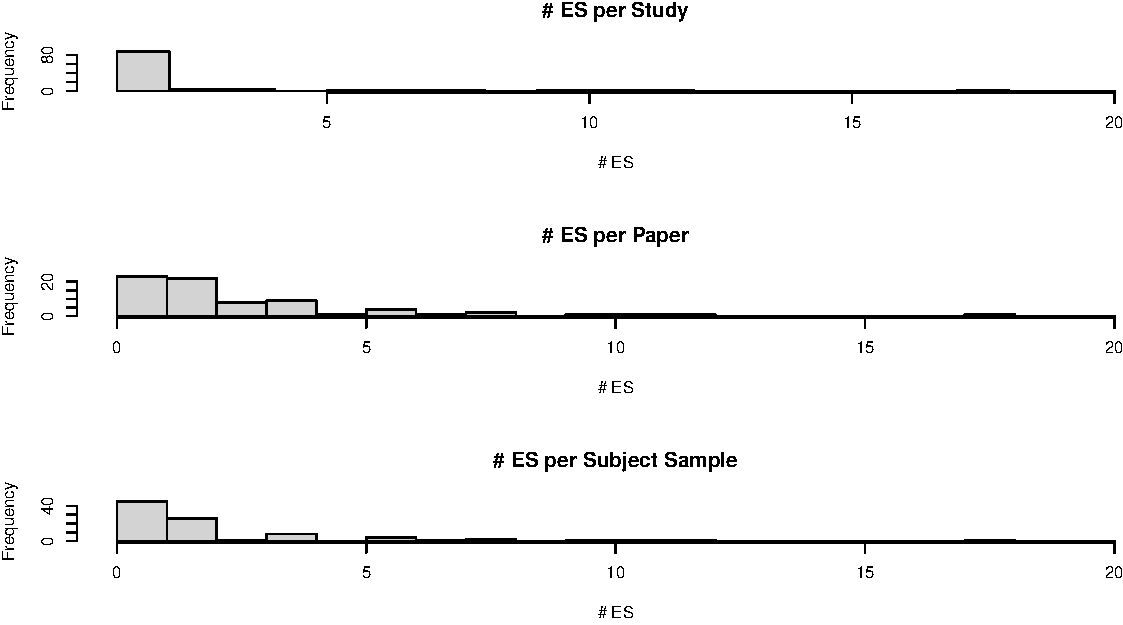
\includegraphics{MetaAnalysis_CrossSectional_files/figure-latex/EShistograms-1.pdf}

Most studies contributed only few effects.

\begin{center}\rule{0.5\linewidth}{0.5pt}\end{center}

Notes:\\
- Studies are embedded in Papers.\\
- There are cases of overlap in participants across studies and papers\\
o Studies reported in a paper can involve overlapping samples of participants\\
o Samples of participants (complete or partial) can be reported in several studies or papers

\begin{center}\rule{0.5\linewidth}{0.5pt}\end{center}

\hypertarget{moderators}{%
\section{Moderators}\label{moderators}}

\begin{tabular}{l|l|r}
\hline
Moderator & Level & n\\
\hline
 & bottom-up attention & 9\\
\cline{2-3}
 & inhibition & 10\\
\cline{2-3}
 & motor control & 3\\
\cline{2-3}
 & multi-tasking & 24\\
\cline{2-3}
 & perception & 38\\
\cline{2-3}
 & problem solving & 8\\
\cline{2-3}
 & spatial cognition & 29\\
\cline{2-3}
 & top-down attention & 78\\
\cline{2-3}
\multirow[t]{-9}{*}{\raggedright\arraybackslash Cognitive\_domain} & verbal cognition & 31\\
\cline{1-3}
 & accuracy & 123\\
\cline{2-3}
\multirow[t]{-2}{*}{\raggedright\arraybackslash DV\_type} & speed & 107\\
\cline{1-3}
 & interaction & 67\\
\cline{2-3}
\multirow[t]{-2}{*}{\raggedright\arraybackslash Effect} & main & 163\\
\cline{1-3}
 & Covert & 32\\
\cline{2-3}
 & Overt & 196\\
\cline{2-3}
\multirow[t]{-3}{*}{\raggedright\arraybackslash Recruitment} & Recruitment!? & 2\\
\hline
\end{tabular}

\begin{quote}
\emph{note: problematic levels will be recoded before moderator analysis}
\end{quote}

\hypertarget{number-of-effect-sizes-and-studies-i.e.-manuscript-in-each-cognitive-domain}{%
\subsection{Number of effect sizes and studies (i.e.~manuscript) in each cognitive domain}\label{number-of-effect-sizes-and-studies-i.e.-manuscript-in-each-cognitive-domain}}

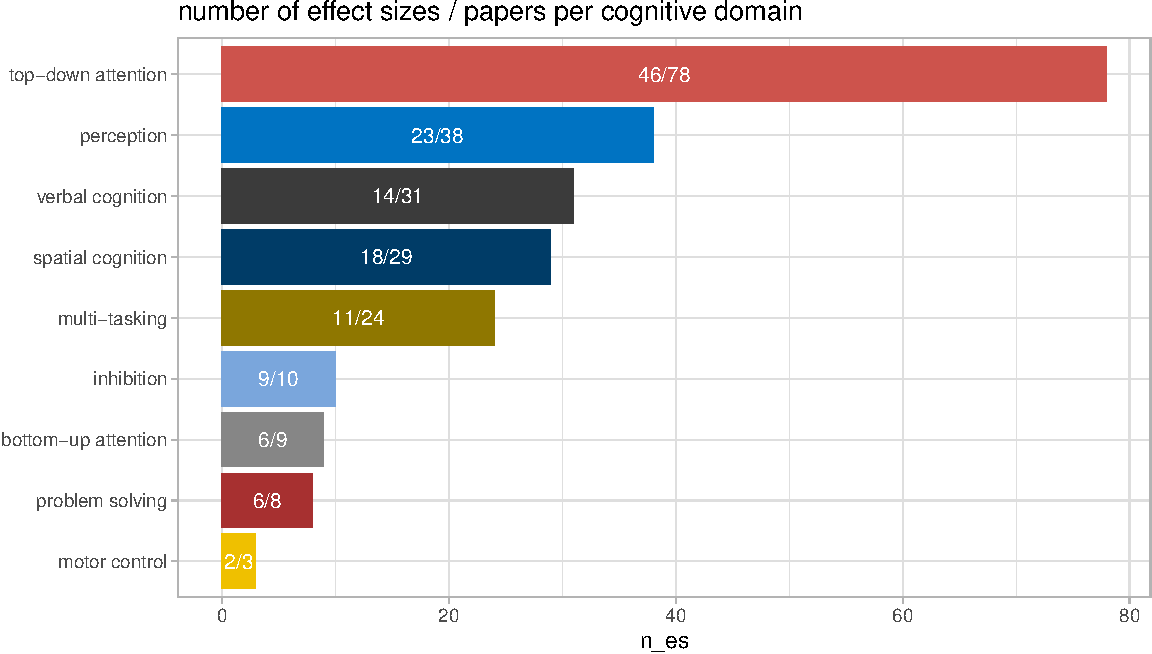
\includegraphics{MetaAnalysis_CrossSectional_files/figure-latex/nESbyCogDom-1.pdf}

\hypertarget{list-of-tasks-and-cognitive-domains}{%
\subsection{List of Tasks and Cognitive Domains}\label{list-of-tasks-and-cognitive-domains}}

Click to expand!

\begin{tabular}{l|l|l}
\hline
Cognitive\_domain & examples & measures\\
\hline
 & Audio-Visual simultaneity judgment & Group: point of subjective simultaneity (Gaussian fitting) in ms\\
\cline{2-3}
 & Audio-Visual temporal-order judgment & Group: just noticeable difference (Sigmoid fitting) in ms\\
\cline{2-3}
 & Auditory Tone Location discrimination & Main effect : Model fitting : DDM Model Parameters: Integration rate\\
\cline{2-3}
 & Auditory Tone Location discrimination - critical duration & Main effect : Model fitting : Model Parameters: beta/rate at which accuracy grows as a function of time\\
\cline{2-3}
 & Baseline task (BAS) & Main effect : accuracy rate (\% correct)\\
\cline{2-3}
 & Baseline task (BAS) & Main effect : reaction time (ms)\\
\cline{2-3}
 & Binocular Rivalry - dynamic stim & alternations (passiv dynamic)\\
\cline{2-3}
 & Binocular Rivalry - static stim & alternations (passiv static)\\
\cline{2-3}
 & Bissection task & Main effect : accuracy (absolute deviation)\\
\cline{2-3}
 & Choice RT - single task & Group: RT\\
\cline{2-3}
 & combiTVA & Main effect : t0 (lower = better)\\
\cline{2-3}
 & Compound search - Target discrimination & Main effect Group: Group x onset presence: manual RT\\
\cline{2-3}
 & Compound search - Target discrimination & Main effect Group: Group x Onset presence: Manual RT\\
\cline{2-3}
 & Contrast Sensitivity & Main effect : sensitivity\\
\cline{2-3}
 & Contrast Sensitivity - critical duration & Main effect : critical duration\\
\cline{2-3}
 & Crowding paradigm - acuity (T-alone discrimination accuracy) & Main effect Group: Group x eccentricity: T-alone discrimination accuracy\\
\cline{2-3}
 & Crowding paradigm - crowding & Main effect Group: Group x eccentricity: log10 distance threshold\\
\cline{2-3}
 & Flicker fusion & Main effect : thresholds (Freq threshold (84\% correct) in Hz)\\
\cline{2-3}
 & Masked prime visibility - prime discrimination: categorize as larger / smaller than reference frame & Main effect : d' (prime 20 or 60 ms)\\
\cline{2-3}
 & Masked priming - target discrimination: categorize as larger / smaller than reference frame & Main effect : RT (prime 20 or 60 ms)\\
\cline{2-3}
 & Masking (backward colinear) & main effect Group\\
\cline{2-3}
 & Masking (backward orthogonal) & main effect Group\\
\cline{2-3}
 & Masking (forward and backward / lateral) & main effect Group\\
\cline{2-3}
 & Modified attentional-blink task (local) & Main effect: Group  T1 accuracy\\
\cline{2-3}
 & Modified attentional-blink task (local) & Main effect: Group: T1 identification\\
\cline{2-3}
 & Motion Perception (up/down, expansion/contraction, clockwise/anticlockwise) & Main effect : Motion coherence threshold (level of coherence required to achieve 79\% correct)\\
\cline{2-3}
 & Motion Perception: radial (contraction) & Main effect (contraction) : Motion coherence threshold (level of coherence required to achieve 79\% correct)\\
\cline{2-3}
 & Motion Perception: radial (expansion) & Main effect (expansion) : Motion coherence threshold (level of coherence required to achieve 79\% correct)\\
\cline{2-3}
 & Orientation Identification & Main effect: contrast threshold\\
\cline{2-3}
 & Perceptual Discrimination RT & Main effect of Group: RT\\
\cline{2-3}
 & Posner Name Identity & Main effect: Group : RT difference between Name identity and Physical identity (p>.4)\\
\cline{2-3}
 & Simple RT & Main effect of Group: RT\\
\cline{2-3}
 & Temporal Order Judgment & Main effect : Point of Subjective Simultaneity (ms)\\
\cline{2-3}
 & TVA whole & Main effect : threshold (minimum presentation, parameter t0)\\
\cline{2-3}
 & UFOV - single\&dual task / no distractors / peripheral task & Main effect Group (ANOVA : Group x eccentricity x center task): Peripheral localization accuracy \%\\
\cline{2-3}
 & Visual Motion Direction discrimination & Main effect : DDM Model Parameters: Integration rate\\
\cline{2-3}
 & Visual Motion Direction discrimination - critical duration & Main effect : Model fitting : Model Parameters: beta/rate at which accuracy grows as a function of time\\
\cline{2-3}
\multirow[t]{-38}{*}{\raggedright\arraybackslash perception} & Visual search (a la Chisholm) & Main effect : RT\\
\cline{1-3}
 & Lane-keeping task & Main effect : mean root mean square (RMS) of the vehicular lateral deviation (in meters)\\
\cline{2-3}
 & Manual motion-tracking task & Main effect : mean deviation per cycle\\
\cline{2-3}
\multirow[t]{-3}{*}{\raggedright\arraybackslash motor control} & Visuo-motor control task & Main effect : mean RMS target position error (°)\\
\cline{1-3}
 & ANT: Attentional Network Test & Alerting effect: RT (nocue - double)\\
\cline{2-3}
 & ANT: Attentional Network Test & alerting RT\\
\cline{2-3}
 & ANT: Attentional Network Test & Orienting effect: RT(center - orienting)\\
\cline{2-3}
 & ANT: Attentional Network Test & orienting RT\\
\cline{2-3}
 & classical Visual search (color) & Main effect (color task) : RT (AVERAGE ACROSS 3 SET SIZES)\\
\cline{2-3}
 & classical Visual search (orientation) & Main effect (orientation task) : RT (AVERAGE ACROSS 3 SET SIZES)\\
\cline{2-3}
 & Inattentional Blindness & Main effect : inattention condition : \% inattentional blindness\\
\cline{2-3}
 & Modified Posner Cueing (exogenous cue) & Interaction : group x cue validity x SOA : RT (mean) in ms\\
\cline{2-3}
\multirow[t]{-9}{*}{\raggedright\arraybackslash bottom-up attention} & Posner (exogenous) Cue-Target & Interaction: Group x cue validity x SOA: RT\\
\cline{1-3}
 & ANT: Attentional Network Test & Conflict effect (RT inc - RT cong)\\
\cline{2-3}
 & ANT: Attentional Network Test & conflict RT\\
\cline{2-3}
 & Antisaccade & Main effect : anti\_err (proportion of errors)\\
\cline{2-3}
 & Attentional Blink & Main effect of Group - accuracy\\
\cline{2-3}
 & Attentional Blink & Main effect of Group:  T2 accuracy (T1 correct) with lag\\
\cline{2-3}
 & Attentional/Oculomotor capture & Interaction: Group x awareness: oculomotor capture \%\\
\cline{2-3}
 & Attentional/Oculomotor capture & Interaction: Group x onset presence: first-saccade accuracy = \% initial saccades to the abrupt onset\\
\cline{2-3}
 & Attentional/Oculomotor capture (Target orientation discrimination with/out distractors) & Interaction: Group x distractor presence: RT\\
\cline{2-3}
 & Attentional/Oculomotor capture with schematic emotional stimuli & Interaction: Group x onset presence: Saccade accuracy\\
\cline{2-3}
 & Auditory target detection task (focused vs divided) & Main effect : group : d prime scores\\
\cline{2-3}
 & AX CPT & Main effect: efficiency index\\
\cline{2-3}
 & Binocular Rivalry - dynamic stim & Interaction: attended duration (task vs passiv dynamic): \%-change of median\\
\cline{2-3}
 & Binocular Rivalry - dynamic stim & Interaction: unattended duration (task vs passiv dynamic): \%-change of median\\
\cline{2-3}
 & Binocular Rivalry - static stim & Interaction: attended duration (hold vs passiv static) \%-change of median\\
\cline{2-3}
 & Binocular Rivalry - static stim & Interaction: unattended duration (hold vs passiv static): \%-change of median\\
\cline{2-3}
 & Change detection & Main effect : Arrays\_k (bias-corrected measure of capacity : k)\\
\cline{2-3}
 & Change detection & Main effect : number of detected changes\\
\cline{2-3}
 & Change detection & Number of cycles required to find change (change trials)\\
\cline{2-3}
 & Change detection (abrupt change in motion) & Main effect : sensitivity (d')\\
\cline{2-3}
 & classical Visual search (conjunction) & Main effect (conjunction task) : search slopes (ms/item) - RT fitted on the number of items\\
\cline{2-3}
 & combiTVA & Main effect : alpha (lower = better)\\
\cline{2-3}
 & combiTVA & Main effect : C (higher = better)\\
\cline{2-3}
 & Compound search & Interaction: Group x onset presence: Saccade accuracy\\
\cline{2-3}
 & Cued visual search & Main effect : CuedSrch.RT\_mean (mean RT for correct responses)\\
\cline{2-3}
 & D2 attention & Main effect: group (accuracy)\\
\cline{2-3}
 & D2 concentration & Main effect: group (accuracy)\\
\cline{2-3}
 & D2-Test & Main effect : accuracy\\
\cline{2-3}
 & Digit detection & Main effect : scores\\
\cline{2-3}
 & Distractor Filtering & Main effect: RT\\
\cline{2-3}
 & Eriksen flanker task & Main effect : RT (within 200-1800 ms range)\\
\cline{2-3}
 & Flanker task & Group: interference cost (RT incongruent - RT congruent)\\
\cline{2-3}
 & Flanker task & Main effect : accuracy (\% correct)\\
\cline{2-3}
 & Flanker task & Main effect : ArrFlnkINC\_CON (RT difference between incongruent and congruent trials)\\
\cline{2-3}
 & Flanker task high load (lower cost = better) & Interaction Group x Compatibility @ load 6 (lower = better): flanker compability effect (RT compatible - RT incompatible)\\
\cline{2-3}
 & Flanker task low load (higher cost = better) & Interaction Group x Compatibility @ load 1 (higher = better): flanker compability effect (RT compatible - RT incompatible)\\
\cline{2-3}
 & MIT task (multiple identity tracking) & Main effect : accuracy (nb items tracked) - specific condition\\
\cline{2-3}
 & MIT task (multiple identity tracking) & Main effect : accuracy (nb items tracked) - standard condition\\
\cline{2-3}
 & Modified attentional-blink task (local) & Main effect: Group : T2 accuracy / T1 correct (dprime)\\
\cline{2-3}
 & MOT & Main effect : accuracy\\
\cline{2-3}
 & MOT & Main effect Group: Group x Number of circles: \% correct\\
\cline{2-3}
 & MOT & Main effect of Group: accuracy 1-5 dots\\
\cline{2-3}
 & N2pc task & Main effect : frequent color/response vs infrequent color/response (\% correct)\\
\cline{2-3}
 & Oculomotor visual search & Main effect Group\\
\cline{2-3}
 & Perceptual load paradigm & Interaction: Group x Perceptual Load x Distractor Compatibility: filtered RT\\
\cline{2-3}
 & Peripheral search alone - reciprocal-transformed RT - peripheral search alone & Main effect (peripheral search alone) : reciprocal-transformed RT\\
\cline{2-3}
 & Saccadic trajectory deviation task & Main effect : accuracy - percentage of saccades that were erroneously directed to the distractor\\
\cline{2-3}
 & search task & main effect: error\\
\cline{2-3}
 & search task & main effect: RT\\
\cline{2-3}
 & search task & search accuracy\\
\cline{2-3}
 & search task & search time\\
\cline{2-3}
 & Successive series & Main effect : scores\\
\cline{2-3}
 & SVST - inefficiency index & Main effect : SVST - inefficiency index\\
\cline{2-3}
 & Target detection (SSVEP) & Main effect : RT\\
\cline{2-3}
 & Target detection task (Cued/uncued with/out distractors) & Main effect : group (target present trials) : inverse efficiency score\\
\cline{2-3}
 & Target detection task (focused vs divided) & Main effect : RT\\
\cline{2-3}
 & Target discrimination (Low vs High Load x Central vs Peripheral distractors) & Main effect: RT\\
\cline{2-3}
 & TOVA sustained & Main effect : (Target Frequency Condition) : sustained attention RT (msec)\\
\cline{2-3}
 & TOVA sustained & Main effect of Group: RT\\
\cline{2-3}
 & TVA partial & Main effect : top-down control (alpha)\\
\cline{2-3}
 & TVA whole & Main effect : processing speed (slope, parameter C)\\
\cline{2-3}
 & UFOV & main effect of group: threshold\\
\cline{2-3}
 & UFOV - single task / with distractors / peripheral task & Main effect : proportion of accurate responses\\
\cline{2-3}
 & UFOV - single task / with distractors / peripheral task alone & Group: percent correct localization accuracy\\
\cline{2-3}
 & UFOV - single task / with distractors / peripheral task alone & Main effect Group: Group x Gender x Field of study: \% correct responses\\
\cline{2-3}
 & UFOV - single\&dual task / with distractors / peripheral task & Main effect Group (ANOVA :Group x eccentricity x center task) Peripheral localization accuracy \%\\
\cline{2-3}
 & UFOV (FFOV) - single task / with distractor / peripheral task alone & Group: percentage correct (peripheral targets)\\
\cline{2-3}
 & VAST & Main effect : VAST\\
\cline{2-3}
 & Visual search & Main effect : RT\\
\cline{2-3}
 & Visual search & Main effect : scores\\
\cline{2-3}
 & Visual search & Main effect of Group: RT\\
\cline{2-3}
 & Visual search & Main effect: RT\\
\cline{2-3}
 & Visual search (a la Chisholm) & Interaction Group x Distractor presence: RT\\
\cline{2-3}
 & Visual search (EXP1A: self paced) & Main effect : search rates (ms/items)\\
\cline{2-3}
 & Visual search (EXP1B: critical duration) & Main effect : search rates (ms/items)\\
\cline{2-3}
\multirow[t]{-75}{*}{\raggedright\arraybackslash top-down attention} & Visual search (low / high task difficulty - no feature in common between target and distractors or 1 feature in common between distractor and target : either size or color, low / high background difficulty) & Main effect : RT\\
\cline{1-3}
 & Countermanding saccade - SSRT & Main effect : SSRT (Stop-signal reaction time on noGo trials)\\
\cline{2-3}
 & Proactive Interference & Main effect : RT normalized (=RT/proportion correct)\\
\cline{2-3}
 & SART & Main effect : SART.RT\_trim\_ISD (standard deviation of response time on go trials)\\
\cline{2-3}
 & Spatial stroop & Main effect : SpStrpINC\_CON (RT difference between incongruent and congruent trials)\\
\cline{2-3}
 & Stop-change paradigm (Go/Stop-change delay = 0ms / stop-change delay = 300ms) & Main effect : Mean stop signal RT (SSRT)\\
\cline{2-3}
 & Stop-signal task & Mean stop-signal RT\\
\cline{2-3}
 & Stroop & Main effect of Group: Incongruent RT - Congruent RT\\
\cline{2-3}
 & Target detection task (Cued/uncued with/out distractors) & Main effect : group (catch trials) : false alarm (FA) rates \%\\
\cline{2-3}
 & TOVA impulsive & Main effect : (Target Frequency Condition) : impulsivity RT (msec)\\
\cline{2-3}
\multirow[t]{-10}{*}{\raggedright\arraybackslash inhibition} & TOVA impulsive & Main effect of Group: RT\\
\cline{1-3}
 & 4/8 maze task & Main effect : VR task with response > spatial learning strategies (\% of participants using response strategy)\\
\cline{2-3}
 & Change detection - Varying the cue-to-memory-array delay (Task 1) & Main effect : ratio of correct responses to the total number of trials\\
\cline{2-3}
 & Change detection - Varying the test-array-to-cue delay (Task 2) & Main effect : accuracy\\
\cline{2-3}
 & Change detection - Varying the test-array-to-cue delay (Task 2) & Main effect : ratio of correct responses to the total number of trials\\
\cline{2-3}
 & Color wheel task & Main effect : accuracy (average error)\\
\cline{2-3}
 & Corsi block-tapping task (CBTT) single & Main effect : RT single task\\
\cline{2-3}
 & Enumeration & Main effect : breakpoint Acc 50ms MASKED\\
\cline{2-3}
 & Enumeration & Main effect : breakpoint RT 100ms MASKED\\
\cline{2-3}
 & Enumeration & Main effect : breakpoint RT 50ms UNMASKED\\
\cline{2-3}
 & Enumeration & Main effect Group: Group x Field of view: nb of items subitized\\
\cline{2-3}
 & Enumeration & nb of items subitized\\
\cline{2-3}
 & Enumeration (with MASK) & Main effect Group: Group x Field of view: nb of items subitized\\
\cline{2-3}
 & Filter task & capacity K\\
\cline{2-3}
 & Interception & hits\\
\cline{2-3}
 & Matrix monitoring & Main effect : MatMon.acc (proportion of correct responses)\\
\cline{2-3}
 & Memory Task & Main effect of group: accuracy (\%correct)\\
\cline{2-3}
 & Mental Rotation & RT\\
\cline{2-3}
 & Mental Rotation & RT/accuracy\\
\cline{2-3}
 & N-Back (single task) & Main effect : RT Single task\\
\cline{2-3}
 & Race & RT/accuracy\\
\cline{2-3}
 & Rotation span & Main effect : MaxRotSpanTotal (total number of arrows recalled in the correct order)\\
\cline{2-3}
 & Symmetry span & Main effect : MaxSspanTotal (locations correctly recalled)\\
\cline{2-3}
 & Visual Short Term Memory (VSTM) & Group: percentage correct\\
\cline{2-3}
 & Visual Short Term Memory (VSTM) & Interaction : Group x set size : d prime\\
\cline{2-3}
 & Visual Short Term Memory (VSTM) & Main effect of group at Time 1\\
\cline{2-3}
 & Visual Short Term Memory (VSTM) / change detection COMPLEX & Main effect: accuracy\\
\cline{2-3}
 & Visual Short Term Memory (VSTM) / change detection SIMPLE & Main effect: accuracy\\
\cline{2-3}
\multirow[t]{-28}{*}{\raggedright\arraybackslash spatial cognition} & Visuospatial task (VST) & Main effect : accuracy rate (\% correct)\\
\cline{1-3}
 & Auditory 2 back during street crossing (VR CAVE):  dual task - single task cost & dual task cost accuracy\\
\cline{2-3}
 & Computer dual task & Interaction: Group x task (single vs. dual): RT\\
\cline{2-3}
 & Corsi block-tapping task (CBTT) dual task cost & Main effect : accuracy Dual task - Single Task\\
\cline{2-3}
 & Distracted driving task & Main effect : D2-D1 cost (untransformed lane deviation values)\\
\cline{2-3}
 & Dual task (visual or auditory) & Main effect : dual task (SOA 50) - task 1 : RT\\
\cline{2-3}
 & Dual task (visual or auditory) & Main effect : dual task (SOA 50) - task 2 : RT\\
\cline{2-3}
 & dual visual search - central task & Main effect (central component of dual search) : accuracy (arcsine-transformed proportion of correct responses)\\
\cline{2-3}
 & dual visual search - peripheral task & Main effect (peripheral component of dual search) : reciprocal-transformed RT\\
\cline{2-3}
 & N-Back (dual - single task) & Main effect : RT Dual task - Single Task\\
\cline{2-3}
 & Street Crossing - crossing success & dual task cost\\
\cline{2-3}
 & Street Crossing - crossing time & dual task cost\\
\cline{2-3}
 & Street Crossing - head turns & dual task cost\\
\cline{2-3}
 & Street Crossing - preparation time & dual task cost\\
\cline{2-3}
 & Street Crossing - time to contact & dual task cost\\
\cline{2-3}
 & Task switching & Interaction: Group x  task switch (reptition vs. alternation): RT\\
\cline{2-3}
 & Task switching & Switch cost: efficiency index\\
\cline{2-3}
 & Task switching (cognitive vs motor) - unpredictable & Interaction: Group x trial type: median RT\\
\cline{2-3}
 & Task switching (cognitive) - predictable sequence & Interaction: Group x trial type: median RT\\
\cline{2-3}
 & Task switching (odd/even, prime number or not, larger or smaller than 5) & Interaction : group x switch (repeat, 1-switch, 2-switch, alternate) : raw RT data (within 300-5000 ms range)\\
\cline{2-3}
 & Task switching (perceptual) - predictable sequence & Interaction: Group x trial type: median RT\\
\cline{2-3}
 & Task switching (speeded responses to one of six single-character stimuli, under a range of intermixed stimulus, response, cuing and timing conditions) & Interaction : group x task switching (repeat vs switch) : raw RT data (within 250-2000 ms range)\\
\cline{2-3}
 & Trail Making Test (B - A) & Interaction Group x Task: time to complete TMTB - TMTA\\
\cline{2-3}
\multirow[t]{-23}{*}{\raggedright\arraybackslash multi-tasking} & UFOV dual task  / no distractors / central task & Main effect Group (ANOVA : Group x eccentricity x center task) : center identification accuracy \%\\
\cline{1-3}
 & Auditory 2 back - single task 2-back & \% correct\\
\cline{2-3}
 & combiTVA & Main effect : K (higher = better)\\
\cline{2-3}
 & Continuous counters & Main effect : Counters.ACC (proportion of correct final counts)\\
\cline{2-3}
 & Digit symbol coding (Wechsler) & Main effect : accuracy\\
\cline{2-3}
 & Digits forward span & Main effect : scores\\
\cline{2-3}
 & DSPAN & main effect of group: score\\
\cline{2-3}
 & Keeping track & Main effect : KeepTrack (total number of correctly recalled final exemplars)\\
\cline{2-3}
 & Letter detection task (LDT) & Main effect : accuracy rate (\% correct)\\
\cline{2-3}
 & N-Back & 1-back accuracy\\
\cline{2-3}
 & N-Back & 2-back accuracy\\
\cline{2-3}
 & N-Back & Main effect of Group: RT\\
\cline{2-3}
 & N-Back & Main effect: efficiency index\\
\cline{2-3}
 & N-Back (excluding the 1 back condition) & Main effect : RT (excluding the 1 back condition)\\
\cline{2-3}
 & Nelson Denny & Main effect : Nelson Denny - 10 minutes accuracy score (NCE)\\
\cline{2-3}
 & Nelson Denny & Main effect : Nelson Denny - Execution time (seconds)\\
\cline{2-3}
 & Nelson Denny & Main effect : Nelson Denny - Reading rate (NCE)\\
\cline{2-3}
 & Nelson Denny & Main effect : Nelson Denny - Total time accuracy score (NCE)\\
\cline{2-3}
 & Number series & Main effect : MaxNumberSeriesTotal (total number of items solved correctly)\\
\cline{2-3}
 & OSPAN & Main effect : accuracy\\
\cline{2-3}
 & OSPAN & Main effect : MaxOspanTotal\\
\cline{2-3}
 & OSPAN & Main effect : ospan score\\
\cline{2-3}
 & OSPAN & main effect of group: score\\
\cline{2-3}
 & Reading span & Main effect : MaxRspanTotal\\
\cline{2-3}
 & Recall after driving & Main effect : \% of correctly recalled questions\\
\cline{2-3}
 & Sentence reading test & Main effect : number of correct sentences within 3 min\\
\cline{2-3}
 & TOWRE - inefficiency index & Main effect : TOWRE - inefficiency index\\
\cline{2-3}
 & TVA whole & Main effect : capacity k (asymptote)\\
\cline{2-3}
 & TVA whole & Main effect : iconic buffer mu\\
\cline{2-3}
 & Verbal Short Term Memory & Main effect of group at Time 1 for Memory Span\\
\cline{2-3}
\multirow[t]{-30}{*}{\raggedright\arraybackslash verbal cognition} & Visual Brief Report & Main effect : BRTotalScore (total number of letters correctly reported)\\
\cline{1-3}
 & Letter sets & Main effect : MaxLetterSetsTotal (total number of items solved correctly)\\
\cline{2-3}
 & Matrix reasoning (Wechsler) & Main effect : accuracy\\
\cline{2-3}
 & Paper Folding & Main effect : MaxPapFoldTotal (number of problems solved)\\
\cline{2-3}
 & RAVEN (paper and pencil, no time limit) & Main effect : \% corr\\
\cline{2-3}
 & RAVEN (RAPM) & Main effect : MaxRAPMOddTotal (total number of correct solutions)\\
\cline{2-3}
 & RAVEN (RAPM) & main effect of group: score\\
\cline{2-3}
 & RAVEN (SPM) & Group: means of SPM\\
\cline{2-3}
\multirow[t]{-8}{*}{\raggedright\arraybackslash problem solving} & RAVEN short version & Main effect : accuracy\\
\hline
\end{tabular}

\hypertarget{effectsizes}{%
\chapter{Effect Sizes}\label{effectsizes}}

Note: These plots are just raw effect sizes, it is not the output of a meta-analytic model.\\
Effect sizes are NOT corrected for non-independence or weighted by variance or sample size.

\hypertarget{effect-sizes-by-sample-size}{%
\section{Effect sizes by Sample Size}\label{effect-sizes-by-sample-size}}

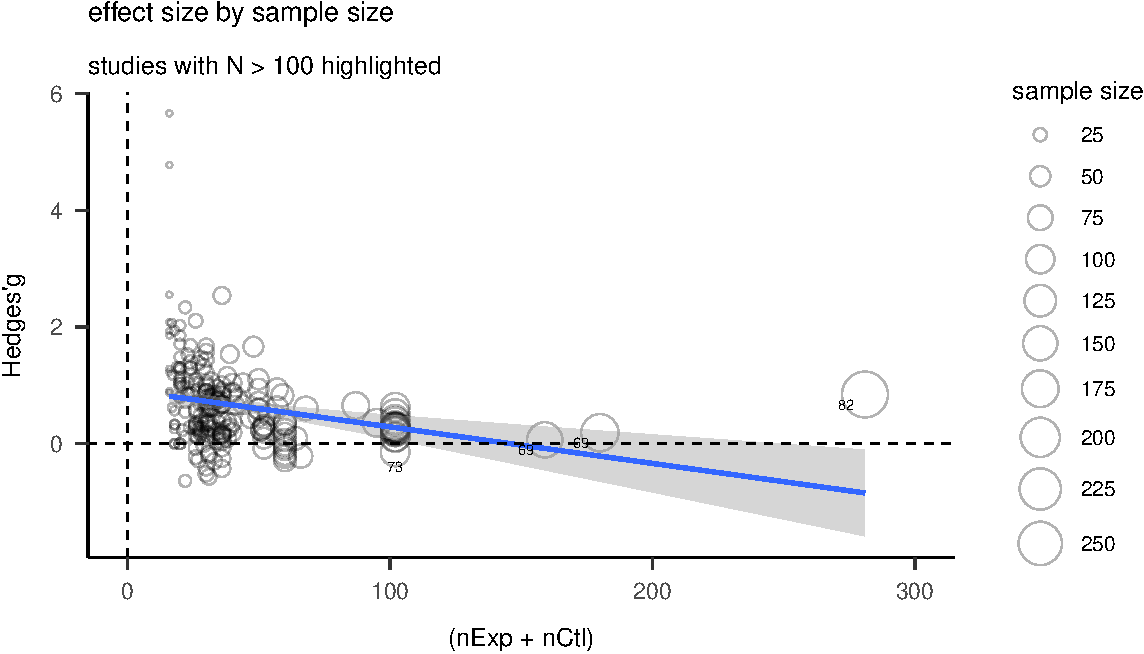
\includegraphics{MetaAnalysis_CrossSectional_files/figure-latex/esByN-1.pdf}
Note: studies with N \textgreater{} 100 are highlighted

\textbf{Studies with N \textgreater{} 100}\\

Click to expand!

\begin{table}
\centering
\begin{tabular}{l|l|l|l|r}
\hline
Paper & Study & Cognitive\_domain & Task & g\\
\hline
69 & Stothart et al VSS poster 2014-EXP1: overt recruit & top-down attention & MOT & 0.068\\
\hline
69 & Stothart et al VSS poster 2014-EXP2: covert recruit & top-down attention & MOT & 0.190\\
\hline
73 & Unsworth et al. 2015-EXP2 / extreme groups - reanalysis & inhibition & SART & 0.276\\
\hline
73 & Unsworth et al. 2015-EXP2 / extreme groups - reanalysis & inhibition & Spatial stroop & 0.310\\
\hline
73 & Unsworth et al. 2015-EXP2 / extreme groups - reanalysis & problem solving & Letter sets & 0.300\\
\hline
73 & Unsworth et al. 2015-EXP2 / extreme groups - reanalysis & problem solving & Paper Folding & 0.273\\
\hline
73 & Unsworth et al. 2015-EXP2 / extreme groups - reanalysis & problem solving & RAVEN (RAPM) & 0.107\\
\hline
73 & Unsworth et al. 2015-EXP2 / extreme groups - reanalysis & spatial cognition & Matrix monitoring & 0.120\\
\hline
73 & Unsworth et al. 2015-EXP2 / extreme groups - reanalysis & spatial cognition & Symmetry span & 0.417\\
\hline
73 & Unsworth et al. 2015-EXP2 / extreme groups - reanalysis & top-down attention & Antisaccade & 0.284\\
\hline
73 & Unsworth et al. 2015-EXP2 / extreme groups - reanalysis & top-down attention & Change detection & 0.377\\
\hline
73 & Unsworth et al. 2015-EXP2 / extreme groups - reanalysis & top-down attention & Cued visual search & 0.242\\
\hline
73 & Unsworth et al. 2015-EXP2 / extreme groups - reanalysis & top-down attention & Flanker task & 0.288\\
\hline
73 & Unsworth et al. 2015-EXP2 / extreme groups - reanalysis & verbal cognition & Continuous counters & 0.214\\
\hline
73 & Unsworth et al. 2015-EXP2 / extreme groups - reanalysis & verbal cognition & Keeping track & -0.140\\
\hline
73 & Unsworth et al. 2015-EXP2 / extreme groups - reanalysis & verbal cognition & Number series & 0.227\\
\hline
73 & Unsworth et al. 2015-EXP2 / extreme groups - reanalysis & verbal cognition & OSPAN & 0.263\\
\hline
73 & Unsworth et al. 2015-EXP2 / extreme groups - reanalysis & verbal cognition & Reading span & 0.203\\
\hline
73 & Unsworth et al. 2015-EXP2 / extreme groups - reanalysis & spatial cognition & Rotation span & 0.626\\
\hline
73 & Unsworth et al. 2015-EXP2 / extreme groups - reanalysis & verbal cognition & Visual Brief Report & 0.516\\
\hline
82 & Caroux 2016 - MALES ONLY & top-down attention & Visual search (low / high task difficulty - no feature in common between target and distractors or 1 feature in common between distractor and target : either size or color, low / high background difficulty) & 0.844\\
\hline
\end{tabular}
\end{table}

\hypertarget{effect-sizes-by-source}{%
\section{Effect sizes by Source}\label{effect-sizes-by-source}}

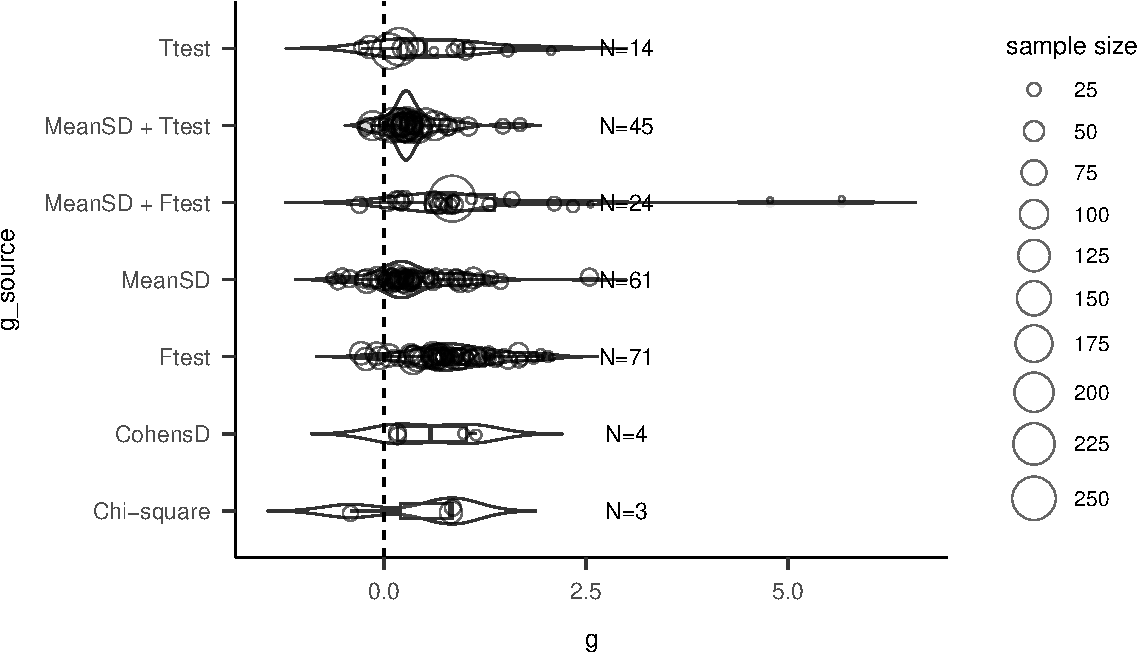
\includegraphics{MetaAnalysis_CrossSectional_files/figure-latex/esByStats-1.pdf}

\hypertarget{effect-sizes-by-cognitive-domain}{%
\section{Effect sizes by Cognitive Domain}\label{effect-sizes-by-cognitive-domain}}

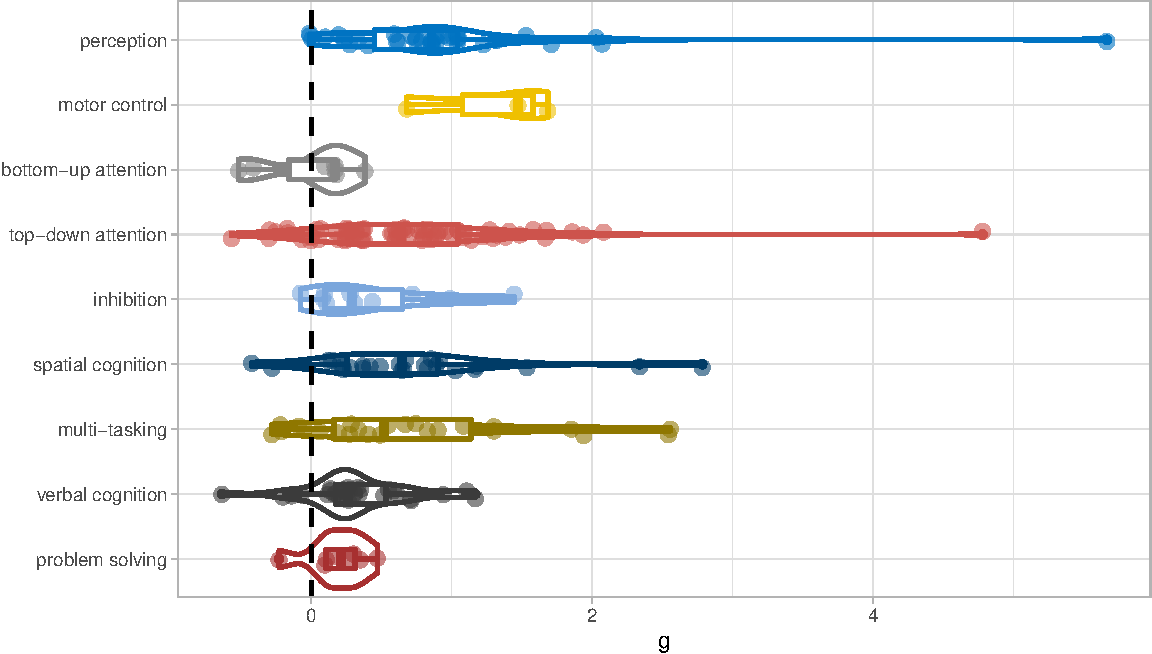
\includegraphics{MetaAnalysis_CrossSectional_files/figure-latex/esByCogDom-1.pdf}

\hypertarget{examine-outliers-and-winsorize}{%
\section{Examine outliers and Winsorize}\label{examine-outliers-and-winsorize}}

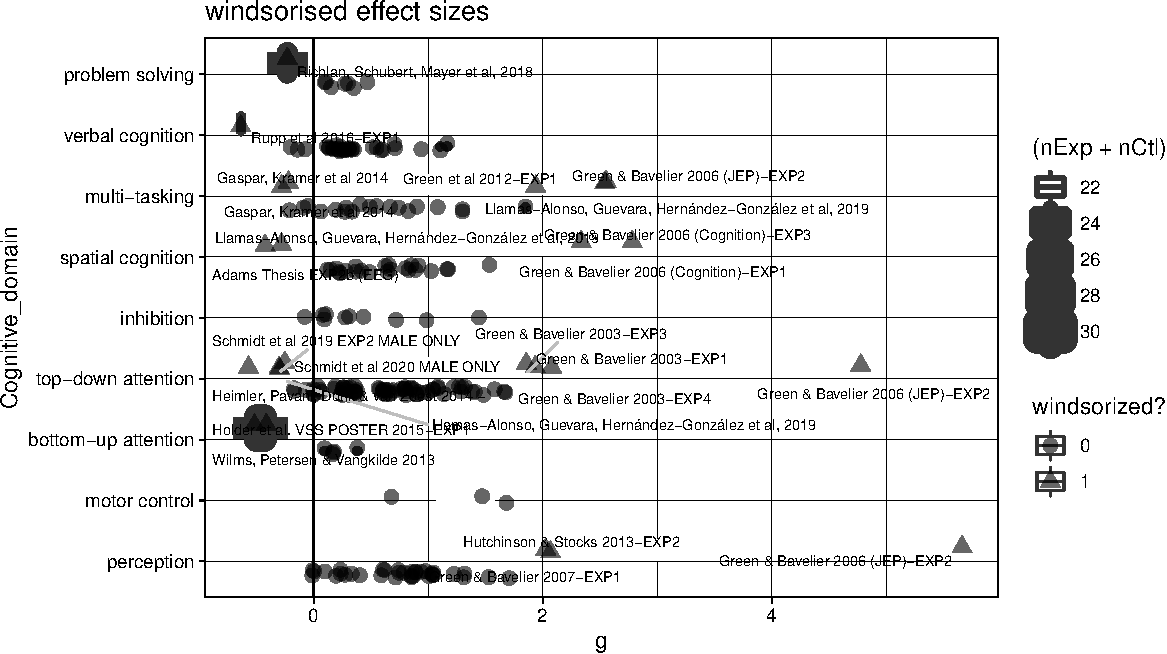
\includegraphics{MetaAnalysis_CrossSectional_files/figure-latex/winsorize-1.pdf}

currently 24 effects winsorized with this approach!

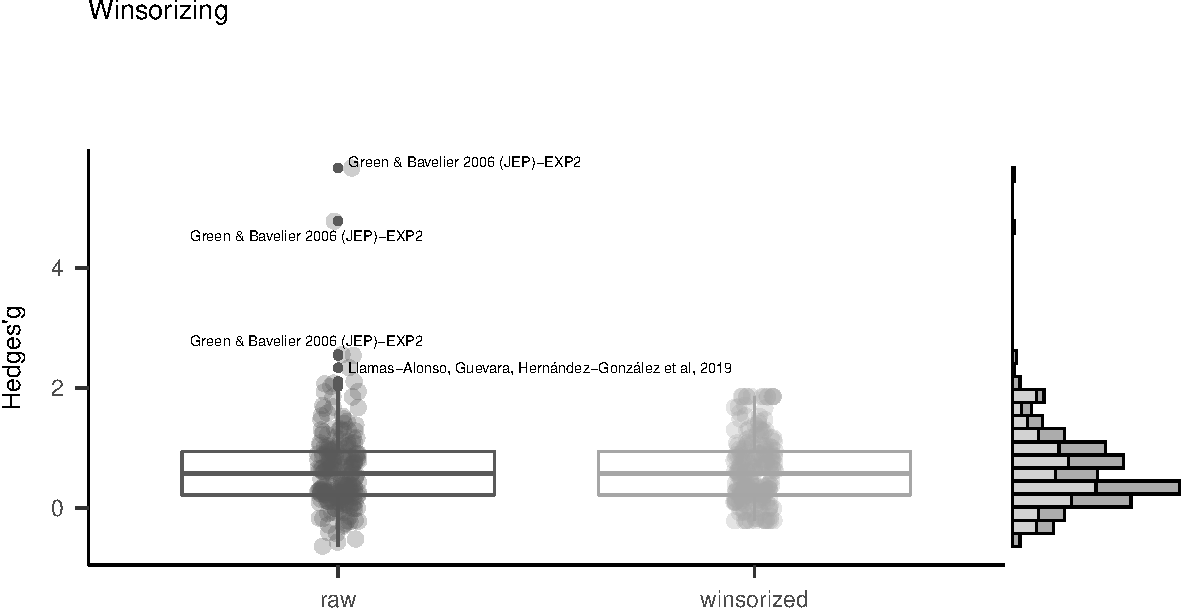
\includegraphics{MetaAnalysis_CrossSectional_files/figure-latex/es_winsorized-1.pdf}

Click to show Winsorized studies!

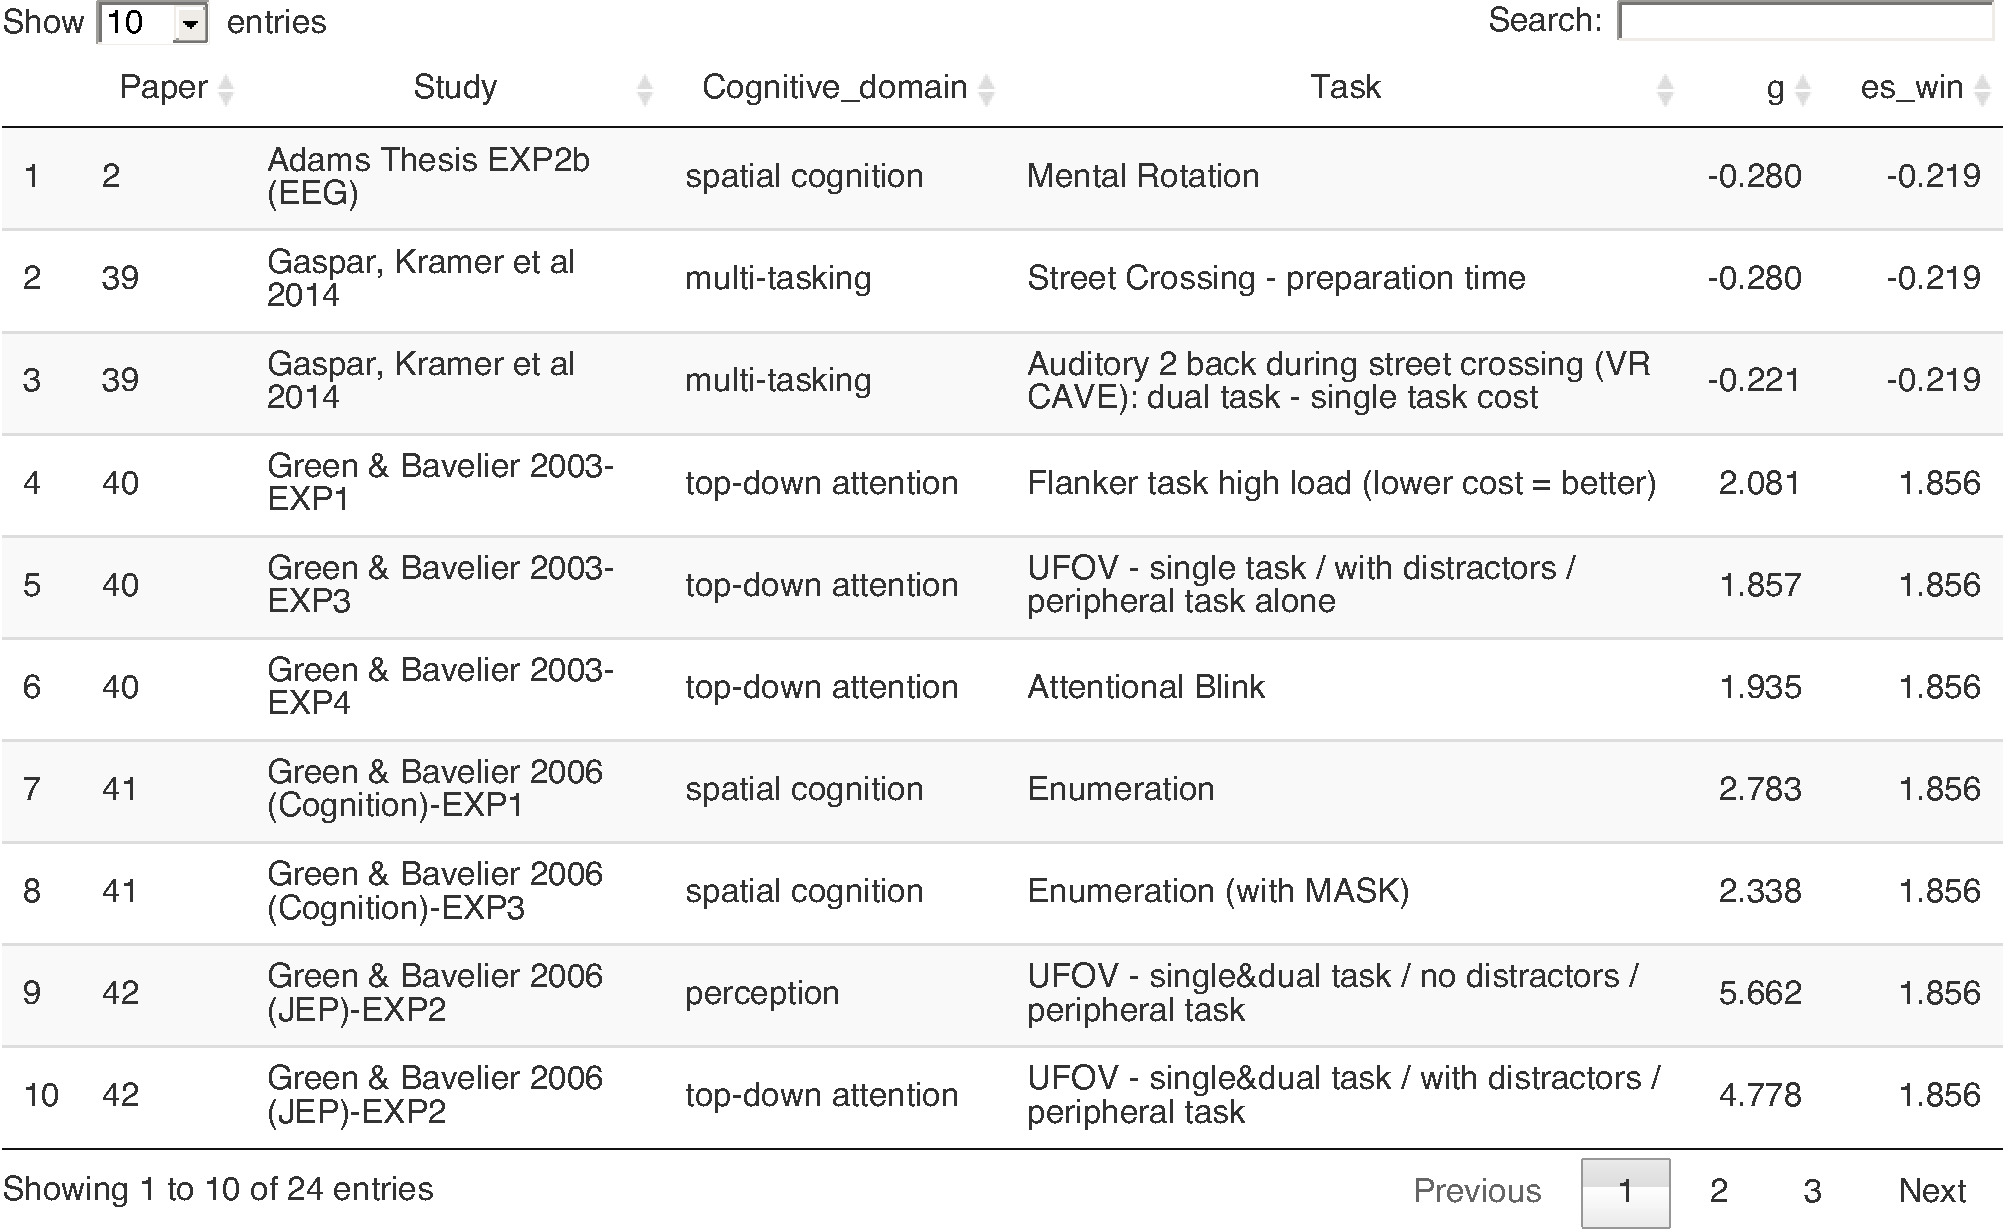
\includegraphics{MetaAnalysis_CrossSectional_files/figure-latex/winstudies-1.pdf}

\hypertarget{final-dataset}{%
\section{Final dataset}\label{final-dataset}}

The analysis is based on 224 effect sizes (vs 194 effect sizes in Bediou et al.~2018).
These ES's were extracted from 102 (vs.~89 in Bediou et al.~2018),
published in 73 manuscripts (vs 73 in Bediou et al.~2018).

The following studies were included in the first MA but excluded in this new MA (see reason).

\begin{longtable}[]{@{}
  >{\raggedright\arraybackslash}p{(\columnwidth - 2\tabcolsep) * \real{0.41}}
  >{\raggedright\arraybackslash}p{(\columnwidth - 2\tabcolsep) * \real{0.59}}@{}}
\toprule
Reference & Reason for exclusion \\
\midrule
\endhead
Appelbaum et al.~2013 & hours NVGP, gender ratio difference \\
Berard, Cain et al 2015 & unmatched gender ratio \\
Bailey et al 2009; 2010; 2012\ldots{} & hours AVGP (total) \\
Buckley et al.~2010 & hours AVGP (range only) \\
Cain et al 2009; 2012; 2014 & unmatched gender ratio \\
Donohue et al.~2012 & hours AVGP (mean 3 h / week + expertise) \\
Dye et al 2009 Neuropsychologia & unmatched gender ratio (ADULT SAMPLE 18-22) \\
Dye et al 2010 ADULTS 18-22 & unmatched gender ratio (ADULT SAMPLE 18-22) \\
Novak \& Tassel 2015 & cannot verify AVGP hours (see email exchanges) \\
Unsworth et al.~2015 EXP1 & Unmatched gender ratio \\
\bottomrule
\end{longtable}

The following manuscripts published after January 2015 were included:\\
list(image = as.raw(c(0x25, 0x50, 0x44, 0x46, 0x2d, 0x31, 0x2e, 0x34, 0x0a, 0x31, 0x20, 0x30, 0x20, 0x6f, 0x62, 0x6a, 0x0a, 0x3c, 0x3c, 0x0a, 0x2f, 0x54, 0x69, 0x74, 0x6c, 0x65, 0x20, 0x28, 0xfe, 0xff, 0x29, 0x0a, 0x2f, 0x43, 0x72, 0x65, 0x61, 0x74, 0x6f, 0x72, 0x20, 0x28, 0xfe, 0xff, 0x29, 0x0a, 0x2f, 0x50, 0x72, 0x6f, 0x64, 0x75, 0x63, 0x65, 0x72, 0x20, 0x28, 0xfe, 0xff, 0x00, 0x51, 0x00, 0x74, 0x00, 0x20, 0x00, 0x35, 0x00, 0x2e, 0x00, 0x35, 0x00, 0x2e, 0x00, 0x31, 0x29, 0x0a, 0x2f, 0x43, 0x72,
0x65, 0x61, 0x74, 0x69, 0x6f, 0x6e, 0x44, 0x61, 0x74, 0x65, 0x20, 0x28, 0x44, 0x3a, 0x32, 0x30, 0x32, 0x31, 0x30, 0x38, 0x30, 0x34, 0x31, 0x30, 0x31, 0x30, 0x31, 0x36, 0x29, 0x0a, 0x3e, 0x3e, 0x0a, 0x65, 0x6e, 0x64, 0x6f, 0x62, 0x6a, 0x0a, 0x32, 0x20, 0x30, 0x20, 0x6f, 0x62, 0x6a, 0x0a, 0x3c, 0x3c, 0x0a, 0x2f, 0x54, 0x79, 0x70, 0x65, 0x20, 0x2f, 0x43, 0x61, 0x74, 0x61, 0x6c, 0x6f, 0x67, 0x0a, 0x2f, 0x50, 0x61, 0x67, 0x65, 0x73, 0x20, 0x33, 0x20, 0x30, 0x20, 0x52, 0x0a, 0x3e, 0x3e, 0x0a, 0x65, 0x6e,
0x64, 0x6f, 0x62, 0x6a, 0x0a, 0x34, 0x20, 0x30, 0x20, 0x6f, 0x62, 0x6a, 0x0a, 0x3c, 0x3c, 0x0a, 0x2f, 0x54, 0x79, 0x70, 0x65, 0x20, 0x2f, 0x45, 0x78, 0x74, 0x47, 0x53, 0x74, 0x61, 0x74, 0x65, 0x0a, 0x2f, 0x53, 0x41, 0x20, 0x74, 0x72, 0x75, 0x65, 0x0a, 0x2f, 0x53, 0x4d, 0x20, 0x30, 0x2e, 0x30, 0x32, 0x0a, 0x2f, 0x63, 0x61, 0x20, 0x31, 0x2e, 0x30, 0x0a, 0x2f, 0x43, 0x41, 0x20, 0x31, 0x2e, 0x30, 0x0a, 0x2f, 0x41, 0x49, 0x53, 0x20, 0x66, 0x61, 0x6c, 0x73, 0x65, 0x0a, 0x2f, 0x53, 0x4d, 0x61, 0x73, 0x6b,
0x20, 0x2f, 0x4e, 0x6f, 0x6e, 0x65, 0x3e, 0x3e, 0x0a, 0x65, 0x6e, 0x64, 0x6f, 0x62, 0x6a, 0x0a, 0x35, 0x20, 0x30, 0x20, 0x6f, 0x62, 0x6a, 0x0a, 0x5b, 0x2f, 0x50, 0x61, 0x74, 0x74, 0x65, 0x72, 0x6e, 0x20, 0x2f, 0x44, 0x65, 0x76, 0x69, 0x63, 0x65, 0x52, 0x47, 0x42, 0x5d, 0x0a, 0x65, 0x6e, 0x64, 0x6f, 0x62, 0x6a, 0x0a, 0x37, 0x20, 0x30, 0x20, 0x6f, 0x62, 0x6a, 0x0a, 0x3c, 0x3c, 0x0a, 0x2f, 0x54, 0x79, 0x70, 0x65, 0x20, 0x2f, 0x58, 0x4f, 0x62, 0x6a, 0x65, 0x63, 0x74, 0x0a, 0x2f, 0x53, 0x75, 0x62, 0x74,
0x79, 0x70, 0x65, 0x20, 0x2f, 0x49, 0x6d, 0x61, 0x67, 0x65, 0x0a, 0x2f, 0x57, 0x69, 0x64, 0x74, 0x68, 0x20, 0x31, 0x39, 0x0a, 0x2f, 0x48, 0x65, 0x69, 0x67, 0x68, 0x74, 0x20, 0x31, 0x39, 0x0a, 0x2f, 0x42, 0x69, 0x74, 0x73, 0x50, 0x65, 0x72, 0x43, 0x6f, 0x6d, 0x70, 0x6f, 0x6e, 0x65, 0x6e, 0x74, 0x20, 0x38, 0x0a, 0x2f, 0x43, 0x6f, 0x6c, 0x6f, 0x72, 0x53, 0x70, 0x61, 0x63, 0x65, 0x20, 0x2f, 0x44, 0x65, 0x76, 0x69, 0x63, 0x65, 0x47, 0x72, 0x61, 0x79, 0x0a, 0x2f, 0x4c, 0x65, 0x6e, 0x67, 0x74, 0x68, 0x20,
0x38, 0x20, 0x30, 0x20, 0x52, 0x0a, 0x2f, 0x46, 0x69, 0x6c, 0x74, 0x65, 0x72, 0x20, 0x2f, 0x46, 0x6c, 0x61, 0x74, 0x65, 0x44, 0x65, 0x63, 0x6f, 0x64, 0x65, 0x0a, 0x3e, 0x3e, 0x0a, 0x73, 0x74, 0x72, 0x65, 0x61, 0x6d, 0x0a, 0x78, 0x9c, 0x63, 0x60, 0x20, 0x05, 0x70, 0x4d, 0x60, 0x43, 0x17, 0x2a, 0xfd, 0x95, 0x8d, 0x26, 0xa2, 0xf5, 0xf8, 0xff, 0x6d, 0x65, 0x14, 0x11, 0xc6, 0xb9, 0xff, 0xff, 0xff, 0x9f, 0xc8, 0x88, 0x2c, 0xe4, 0xf8, 0x0e, 0x28, 0xf4, 0xc9, 0x06, 0x49, 0x84, 0x77, 0xdf, 0x7f, 0x10, 0xd8,
0xc1, 0x8e, 0x10, 0x4a, 0xfc, 0xf9, 0x1d, 0x04, 0x7e, 0x46, 0xe2, 0x75, 0x54, 0x24, 0x54, 0x55, 0x22, 0x42, 0x88, 0x7d, 0x07, 0xd8, 0xac, 0x7d, 0xbc, 0x48, 0xca, 0x6c, 0x3e, 0x01, 0x45, 0xde, 0x39, 0xa2, 0xb8, 0x6b, 0x22, 0x50, 0x68, 0x2e, 0x8a, 0xbb, 0x18, 0x94, 0x6f, 0xff, 0x7f, 0xac, 0x85, 0x66, 0x43, 0xf6, 0xaf, 0x52, 0x74, 0x4b, 0xd9, 0x26, 0x70, 0xe1, 0x75, 0x14, 0x06, 0x00, 0x00, 0x1b, 0x06, 0x3a, 0x1f, 0x65, 0x6e, 0x64, 0x73, 0x74, 0x72, 0x65, 0x61, 0x6d, 0x0a, 0x65, 0x6e, 0x64, 0x6f, 0x62,
0x6a, 0x0a, 0x38, 0x20, 0x30, 0x20, 0x6f, 0x62, 0x6a, 0x0a, 0x31, 0x31, 0x36, 0x0a, 0x65, 0x6e, 0x64, 0x6f, 0x62, 0x6a, 0x0a, 0x39, 0x20, 0x30, 0x20, 0x6f, 0x62, 0x6a, 0x0a, 0x3c, 0x3c, 0x0a, 0x2f, 0x54, 0x79, 0x70, 0x65, 0x20, 0x2f, 0x58, 0x4f, 0x62, 0x6a, 0x65, 0x63, 0x74, 0x0a, 0x2f, 0x53, 0x75, 0x62, 0x74, 0x79, 0x70, 0x65, 0x20, 0x2f, 0x49, 0x6d, 0x61, 0x67, 0x65, 0x0a, 0x2f, 0x57, 0x69, 0x64, 0x74, 0x68, 0x20, 0x31, 0x39, 0x0a, 0x2f, 0x48, 0x65, 0x69, 0x67, 0x68, 0x74, 0x20, 0x31, 0x39, 0x0a,
0x2f, 0x42, 0x69, 0x74, 0x73, 0x50, 0x65, 0x72, 0x43, 0x6f, 0x6d, 0x70, 0x6f, 0x6e, 0x65, 0x6e, 0x74, 0x20, 0x38, 0x0a, 0x2f, 0x43, 0x6f, 0x6c, 0x6f, 0x72, 0x53, 0x70, 0x61, 0x63, 0x65, 0x20, 0x2f, 0x44, 0x65, 0x76, 0x69, 0x63, 0x65, 0x52, 0x47, 0x42, 0x0a, 0x2f, 0x53, 0x4d, 0x61, 0x73, 0x6b, 0x20, 0x37, 0x20, 0x30, 0x20, 0x52, 0x0a, 0x2f, 0x4c, 0x65, 0x6e, 0x67, 0x74, 0x68, 0x20, 0x31, 0x30, 0x20, 0x30, 0x20, 0x52, 0x0a, 0x2f, 0x46, 0x69, 0x6c, 0x74, 0x65, 0x72, 0x20, 0x2f, 0x44, 0x43, 0x54, 0x44,
0x65, 0x63, 0x6f, 0x64, 0x65, 0x0a, 0x3e, 0x3e, 0x0a, 0x73, 0x74, 0x72, 0x65, 0x61, 0x6d, 0x0a, 0xff, 0xd8, 0xff, 0xe0, 0x00, 0x10, 0x4a, 0x46, 0x49, 0x46, 0x00, 0x01, 0x01, 0x01, 0x00, 0x48, 0x00, 0x48, 0x00, 0x00, 0xff, 0xdb, 0x00, 0x43, 0x00, 0x02, 0x01, 0x01, 0x02, 0x01, 0x01, 0x02, 0x02, 0x02, 0x02, 0x02, 0x02, 0x02, 0x02, 0x03, 0x05, 0x03, 0x03, 0x03, 0x03, 0x03, 0x06, 0x04, 0x04, 0x03, 0x05, 0x07, 0x06, 0x07, 0x07, 0x07, 0x06, 0x07, 0x07, 0x08, 0x09, 0x0b, 0x09, 0x08, 0x08, 0x0a, 0x08, 0x07,
0x07, 0x0a, 0x0d, 0x0a, 0x0a, 0x0b, 0x0c, 0x0c, 0x0c, 0x0c, 0x07, 0x09, 0x0e, 0x0f, 0x0d, 0x0c, 0x0e, 0x0b, 0x0c, 0x0c, 0x0c, 0xff, 0xdb, 0x00, 0x43, 0x01, 0x02, 0x02, 0x02, 0x03, 0x03, 0x03, 0x06, 0x03, 0x03, 0x06, 0x0c, 0x08, 0x07, 0x08, 0x0c, 0x0c, 0x0c, 0x0c, 0x0c, 0x0c, 0x0c, 0x0c, 0x0c, 0x0c, 0x0c, 0x0c, 0x0c, 0x0c, 0x0c, 0x0c, 0x0c, 0x0c, 0x0c, 0x0c, 0x0c, 0x0c, 0x0c, 0x0c, 0x0c, 0x0c, 0x0c, 0x0c, 0x0c, 0x0c, 0x0c, 0x0c, 0x0c, 0x0c, 0x0c, 0x0c, 0x0c, 0x0c, 0x0c, 0x0c, 0x0c, 0x0c, 0x0c, 0x0c,
0x0c, 0x0c, 0x0c, 0x0c, 0x0c, 0x0c, 0xff, 0xc0, 0x00, 0x11, 0x08, 0x00, 0x13, 0x00, 0x13, 0x03, 0x01, 0x22, 0x00, 0x02, 0x11, 0x01, 0x03, 0x11, 0x01, 0xff, 0xc4, 0x00, 0x1f, 0x00, 0x00, 0x01, 0x05, 0x01, 0x01, 0x01, 0x01, 0x01, 0x01, 0x00, 0x00, 0x00, 0x00, 0x00, 0x00, 0x00, 0x00, 0x01, 0x02, 0x03, 0x04, 0x05, 0x06, 0x07, 0x08, 0x09, 0x0a, 0x0b, 0xff, 0xc4, 0x00, 0xb5, 0x10, 0x00, 0x02, 0x01, 0x03, 0x03, 0x02, 0x04, 0x03, 0x05, 0x05, 0x04, 0x04, 0x00, 0x00, 0x01, 0x7d, 0x01, 0x02, 0x03, 0x00, 0x04,
0x11, 0x05, 0x12, 0x21, 0x31, 0x41, 0x06, 0x13, 0x51, 0x61, 0x07, 0x22, 0x71, 0x14, 0x32, 0x81, 0x91, 0xa1, 0x08, 0x23, 0x42, 0xb1, 0xc1, 0x15, 0x52, 0xd1, 0xf0, 0x24, 0x33, 0x62, 0x72, 0x82, 0x09, 0x0a, 0x16, 0x17, 0x18, 0x19, 0x1a, 0x25, 0x26, 0x27, 0x28, 0x29, 0x2a, 0x34, 0x35, 0x36, 0x37, 0x38, 0x39, 0x3a, 0x43, 0x44, 0x45, 0x46, 0x47, 0x48, 0x49, 0x4a, 0x53, 0x54, 0x55, 0x56, 0x57, 0x58, 0x59, 0x5a, 0x63, 0x64, 0x65, 0x66, 0x67, 0x68, 0x69, 0x6a, 0x73, 0x74, 0x75, 0x76, 0x77, 0x78, 0x79, 0x7a,
0x83, 0x84, 0x85, 0x86, 0x87, 0x88, 0x89, 0x8a, 0x92, 0x93, 0x94, 0x95, 0x96, 0x97, 0x98, 0x99, 0x9a, 0xa2, 0xa3, 0xa4, 0xa5, 0xa6, 0xa7, 0xa8, 0xa9, 0xaa, 0xb2, 0xb3, 0xb4, 0xb5, 0xb6, 0xb7, 0xb8, 0xb9, 0xba, 0xc2, 0xc3, 0xc4, 0xc5, 0xc6, 0xc7, 0xc8, 0xc9, 0xca, 0xd2, 0xd3, 0xd4, 0xd5, 0xd6, 0xd7, 0xd8, 0xd9, 0xda, 0xe1, 0xe2, 0xe3, 0xe4, 0xe5, 0xe6, 0xe7, 0xe8, 0xe9, 0xea, 0xf1, 0xf2, 0xf3, 0xf4, 0xf5, 0xf6, 0xf7, 0xf8, 0xf9, 0xfa, 0xff, 0xc4, 0x00, 0x1f, 0x01, 0x00, 0x03, 0x01, 0x01, 0x01, 0x01,
0x01, 0x01, 0x01, 0x01, 0x01, 0x00, 0x00, 0x00, 0x00, 0x00, 0x00, 0x01, 0x02, 0x03, 0x04, 0x05, 0x06, 0x07, 0x08, 0x09, 0x0a, 0x0b, 0xff, 0xc4, 0x00, 0xb5, 0x11, 0x00, 0x02, 0x01, 0x02, 0x04, 0x04, 0x03, 0x04, 0x07, 0x05, 0x04, 0x04, 0x00, 0x01, 0x02, 0x77, 0x00, 0x01, 0x02, 0x03, 0x11, 0x04, 0x05, 0x21, 0x31, 0x06, 0x12, 0x41, 0x51, 0x07, 0x61, 0x71, 0x13, 0x22, 0x32, 0x81, 0x08, 0x14, 0x42, 0x91, 0xa1, 0xb1, 0xc1, 0x09, 0x23, 0x33, 0x52, 0xf0, 0x15, 0x62, 0x72, 0xd1, 0x0a, 0x16, 0x24, 0x34, 0xe1,
0x25, 0xf1, 0x17, 0x18, 0x19, 0x1a, 0x26, 0x27, 0x28, 0x29, 0x2a, 0x35, 0x36, 0x37, 0x38, 0x39, 0x3a, 0x43, 0x44, 0x45, 0x46, 0x47, 0x48, 0x49, 0x4a, 0x53, 0x54, 0x55, 0x56, 0x57, 0x58, 0x59, 0x5a, 0x63, 0x64, 0x65, 0x66, 0x67, 0x68, 0x69, 0x6a, 0x73, 0x74, 0x75, 0x76, 0x77, 0x78, 0x79, 0x7a, 0x82, 0x83, 0x84, 0x85, 0x86, 0x87, 0x88, 0x89, 0x8a, 0x92, 0x93, 0x94, 0x95, 0x96, 0x97, 0x98, 0x99, 0x9a, 0xa2, 0xa3, 0xa4, 0xa5, 0xa6, 0xa7, 0xa8, 0xa9, 0xaa, 0xb2, 0xb3, 0xb4, 0xb5, 0xb6, 0xb7, 0xb8, 0xb9,
0xba, 0xc2, 0xc3, 0xc4, 0xc5, 0xc6, 0xc7, 0xc8, 0xc9, 0xca, 0xd2, 0xd3, 0xd4, 0xd5, 0xd6, 0xd7, 0xd8, 0xd9, 0xda, 0xe2, 0xe3, 0xe4, 0xe5, 0xe6, 0xe7, 0xe8, 0xe9, 0xea, 0xf2, 0xf3, 0xf4, 0xf5, 0xf6, 0xf7, 0xf8, 0xf9, 0xfa, 0xff, 0xda, 0x00, 0x0c, 0x03, 0x01, 0x00, 0x02, 0x11, 0x03, 0x11, 0x00, 0x3f, 0x00, 0xfc, 0x6f, 0xff, 0x00, 0x82, 0x75, 0xfe, 0xc2, 0xde, 0x23, 0xff, 0x00, 0x82, 0x8c, 0x7e, 0xd6, 0x1e, 0x1d, 0xf8, 0x5d, 0xe1, 0xdb, 0xb5, 0xd2, 0x3f, 0xb4, 0xc4, 0xb7, 0x7a, 0x9e, 0xb1, 0x2d, 0x9c,
0xd7, 0x56, 0xfa, 0x25, 0x8c, 0x28, 0x5e, 0x5b, 0x89, 0x16, 0x30, 0x79, 0x38, 0x58, 0xa3, 0x0e, 0xc8, 0x8f, 0x34, 0xd0, 0xc6, 0xd2, 0x46, 0x1f, 0x78, 0xfb, 0xe3, 0xfe, 0x0e, 0x1a, 0xff, 0x00, 0x82, 0x21, 0x78, 0x5b, 0xf6, 0x30, 0xf0, 0x4e, 0x85, 0xf1, 0x77, 0xe0, 0xbe, 0x8a, 0x9a, 0x27, 0xc3, 0xd8, 0x1a, 0x0d, 0x0f, 0xc4, 0x3a, 0x0c, 0x52, 0x6a, 0x3a, 0x84, 0xda, 0x7d, 0xd4, 0x8f, 0x33, 0xc5, 0xa9, 0x1b, 0x89, 0xde, 0x60, 0xb6, 0xef, 0xfb, 0xbb, 0x76, 0x0e, 0xf1, 0x84, 0x93, 0xec, 0xe1, 0x44, 0x86,
0x76, 0xf2, 0xfe, 0x5a, 0xff, 0x00, 0x82, 0x19, 0x7c, 0x6c, 0xf8, 0x79, 0xf0, 0x67, 0xf6, 0xf8, 0xd2, 0xe2, 0xf8, 0xa3, 0xad, 0x6b, 0x3e, 0x17, 0xf0, 0x7f, 0x8c, 0x34, 0xbb, 0x9f, 0x0f, 0xcf, 0xae, 0xe9, 0xfe, 0x2f, 0xd5, 0x3c, 0x30, 0x34, 0x69, 0xa4, 0x68, 0xe7, 0x82, 0x59, 0xae, 0x34, 0xf9, 0x23, 0x95, 0xe1, 0x79, 0x6d, 0xd2, 0x16, 0x59, 0x1d, 0x21, 0x4f, 0x3d, 0x66, 0x91, 0x95, 0x60, 0xc8, 0xfd, 0x20, 0xff, 0x00, 0x83, 0x92, 0xae, 0xfe, 0x13, 0x7e, 0xca, 0xdf, 0xb1, 0xe9, 0xf8, 0x7b, 0xa7, 0x78,
0x97, 0xe2, 0x16, 0xb1, 0xf1, 0x23, 0xe2, 0x15, 0xdd, 0x9b, 0x5b, 0x68, 0xba, 0xaf, 0xc5, 0x5f, 0x13, 0x6a, 0xeb, 0x63, 0xa6, 0xc3, 0x71, 0xe7, 0xc9, 0xa8, 0x4d, 0x65, 0x75, 0x77, 0x3d, 0xb4, 0x91, 0x99, 0x6d, 0x96, 0x04, 0x59, 0xc2, 0x92, 0xf2, 0xb4, 0x91, 0x16, 0x6b, 0x67, 0xda, 0x01, 0xf8, 0x39, 0x45, 0x14, 0x50, 0x01, 0x5d, 0x4f, 0xc5, 0xcf, 0x8e, 0x7e, 0x36, 0xf8, 0xff, 0x00, 0xe2, 0x2b, 0x7d, 0x63, 0xc7, 0x9e, 0x31, 0xf1, 0x4f, 0x8d, 0xb5, 0x6b, 0x4b, 0x55, 0xb1, 0x82, 0xf7, 0x5f, 0xd5, 0xa7,
0xd4, 0xae, 0x61, 0xb7, 0x57, 0x77, 0x58, 0x56, 0x49, 0x9d, 0x99, 0x63, 0x0f, 0x24, 0x8c, 0x14, 0x1c, 0x02, 0xec, 0x71, 0x92, 0x68, 0xa2, 0x80, 0x39, 0x6a, 0x28, 0xa2, 0x80, 0x3f, 0xff, 0xd9, 0x65, 0x6e, 0x64, 0x73, 0x74, 0x72, 0x65, 0x61, 0x6d, 0x0a, 0x65, 0x6e, 0x64, 0x6f, 0x62, 0x6a, 0x0a, 0x31, 0x30, 0x20, 0x30, 0x20, 0x6f, 0x62, 0x6a, 0x0a, 0x39, 0x34, 0x30, 0x0a, 0x65, 0x6e, 0x64, 0x6f, 0x62, 0x6a, 0x0a, 0x31, 0x32, 0x20, 0x30, 0x20, 0x6f, 0x62, 0x6a, 0x0a, 0x3c, 0x3c, 0x0a, 0x2f, 0x54, 0x79,
0x70, 0x65, 0x20, 0x2f, 0x58, 0x4f, 0x62, 0x6a, 0x65, 0x63, 0x74, 0x0a, 0x2f, 0x53, 0x75, 0x62, 0x74, 0x79, 0x70, 0x65, 0x20, 0x2f, 0x49, 0x6d, 0x61, 0x67, 0x65, 0x0a, 0x2f, 0x57, 0x69, 0x64, 0x74, 0x68, 0x20, 0x31, 0x30, 0x0a, 0x2f, 0x48, 0x65, 0x69, 0x67, 0x68, 0x74, 0x20, 0x31, 0x30, 0x0a, 0x2f, 0x49, 0x6d, 0x61, 0x67, 0x65, 0x4d, 0x61, 0x73, 0x6b, 0x20, 0x74, 0x72, 0x75, 0x65, 0x0a, 0x2f, 0x44, 0x65, 0x63, 0x6f, 0x64, 0x65, 0x20, 0x5b, 0x31, 0x20, 0x30, 0x5d, 0x0a, 0x2f, 0x4c, 0x65, 0x6e, 0x67,
0x74, 0x68, 0x20, 0x31, 0x33, 0x20, 0x30, 0x20, 0x52, 0x0a, 0x2f, 0x46, 0x69, 0x6c, 0x74, 0x65, 0x72, 0x20, 0x2f, 0x46, 0x6c, 0x61, 0x74, 0x65, 0x44, 0x65, 0x63, 0x6f, 0x64, 0x65, 0x0a, 0x3e, 0x3e, 0x0a, 0x73, 0x74, 0x72, 0x65, 0x61, 0x6d, 0x0a, 0x78, 0x9c, 0x63, 0x60, 0x00, 0x81, 0x7a, 0x06, 0x3b, 0x06, 0x19, 0x06, 0x0e, 0x06, 0x08, 0x00, 0x00, 0x0b, 0x46, 0x00, 0xe2, 0x65, 0x6e, 0x64, 0x73, 0x74, 0x72, 0x65, 0x61, 0x6d, 0x0a, 0x65, 0x6e, 0x64, 0x6f, 0x62, 0x6a, 0x0a, 0x31, 0x33, 0x20, 0x30, 0x20,
0x6f, 0x62, 0x6a, 0x0a, 0x32, 0x31, 0x0a, 0x65, 0x6e, 0x64, 0x6f, 0x62, 0x6a, 0x0a, 0x31, 0x34, 0x20, 0x30, 0x20, 0x6f, 0x62, 0x6a, 0x0a, 0x3c, 0x3c, 0x0a, 0x2f, 0x54, 0x79, 0x70, 0x65, 0x20, 0x2f, 0x58, 0x4f, 0x62, 0x6a, 0x65, 0x63, 0x74, 0x0a, 0x2f, 0x53, 0x75, 0x62, 0x74, 0x79, 0x70, 0x65, 0x20, 0x2f, 0x49, 0x6d, 0x61, 0x67, 0x65, 0x0a, 0x2f, 0x57, 0x69, 0x64, 0x74, 0x68, 0x20, 0x31, 0x30, 0x0a, 0x2f, 0x48, 0x65, 0x69, 0x67, 0x68, 0x74, 0x20, 0x31, 0x30, 0x0a, 0x2f, 0x42, 0x69, 0x74, 0x73, 0x50,
0x65, 0x72, 0x43, 0x6f, 0x6d, 0x70, 0x6f, 0x6e, 0x65, 0x6e, 0x74, 0x20, 0x38, 0x0a, 0x2f, 0x43, 0x6f, 0x6c, 0x6f, 0x72, 0x53, 0x70, 0x61, 0x63, 0x65, 0x20, 0x2f, 0x44, 0x65, 0x76, 0x69, 0x63, 0x65, 0x52, 0x47, 0x42, 0x0a, 0x2f, 0x4d, 0x61, 0x73, 0x6b, 0x20, 0x31, 0x32, 0x20, 0x30, 0x20, 0x52, 0x0a, 0x2f, 0x4c, 0x65, 0x6e, 0x67, 0x74, 0x68, 0x20, 0x31, 0x35, 0x20, 0x30, 0x20, 0x52, 0x0a, 0x2f, 0x46, 0x69, 0x6c, 0x74, 0x65, 0x72, 0x20, 0x2f, 0x44, 0x43, 0x54, 0x44, 0x65, 0x63, 0x6f, 0x64, 0x65, 0x0a,
0x3e, 0x3e, 0x0a, 0x73, 0x74, 0x72, 0x65, 0x61, 0x6d, 0x0a, 0xff, 0xd8, 0xff, 0xe0, 0x00, 0x10, 0x4a, 0x46, 0x49, 0x46, 0x00, 0x01, 0x01, 0x01, 0x00, 0x48, 0x00, 0x48, 0x00, 0x00, 0xff, 0xdb, 0x00, 0x43, 0x00, 0x02, 0x01, 0x01, 0x02, 0x01, 0x01, 0x02, 0x02, 0x02, 0x02, 0x02, 0x02, 0x02, 0x02, 0x03, 0x05, 0x03, 0x03, 0x03, 0x03, 0x03, 0x06, 0x04, 0x04, 0x03, 0x05, 0x07, 0x06, 0x07, 0x07, 0x07, 0x06, 0x07, 0x07, 0x08, 0x09, 0x0b, 0x09, 0x08, 0x08, 0x0a, 0x08, 0x07, 0x07, 0x0a, 0x0d, 0x0a, 0x0a, 0x0b,
0x0c, 0x0c, 0x0c, 0x0c, 0x07, 0x09, 0x0e, 0x0f, 0x0d, 0x0c, 0x0e, 0x0b, 0x0c, 0x0c, 0x0c, 0xff, 0xdb, 0x00, 0x43, 0x01, 0x02, 0x02, 0x02, 0x03, 0x03, 0x03, 0x06, 0x03, 0x03, 0x06, 0x0c, 0x08, 0x07, 0x08, 0x0c, 0x0c, 0x0c, 0x0c, 0x0c, 0x0c, 0x0c, 0x0c, 0x0c, 0x0c, 0x0c, 0x0c, 0x0c, 0x0c, 0x0c, 0x0c, 0x0c, 0x0c, 0x0c, 0x0c, 0x0c, 0x0c, 0x0c, 0x0c, 0x0c, 0x0c, 0x0c, 0x0c, 0x0c, 0x0c, 0x0c, 0x0c, 0x0c, 0x0c, 0x0c, 0x0c, 0x0c, 0x0c, 0x0c, 0x0c, 0x0c, 0x0c, 0x0c, 0x0c, 0x0c, 0x0c, 0x0c, 0x0c, 0x0c, 0x0c,
0xff, 0xc0, 0x00, 0x11, 0x08, 0x00, 0x0a, 0x00, 0x0a, 0x03, 0x01, 0x22, 0x00, 0x02, 0x11, 0x01, 0x03, 0x11, 0x01, 0xff, 0xc4, 0x00, 0x1f, 0x00, 0x00, 0x01, 0x05, 0x01, 0x01, 0x01, 0x01, 0x01, 0x01, 0x00, 0x00, 0x00, 0x00, 0x00, 0x00, 0x00, 0x00, 0x01, 0x02, 0x03, 0x04, 0x05, 0x06, 0x07, 0x08, 0x09, 0x0a, 0x0b, 0xff, 0xc4, 0x00, 0xb5, 0x10, 0x00, 0x02, 0x01, 0x03, 0x03, 0x02, 0x04, 0x03, 0x05, 0x05, 0x04, 0x04, 0x00, 0x00, 0x01, 0x7d, 0x01, 0x02, 0x03, 0x00, 0x04, 0x11, 0x05, 0x12, 0x21, 0x31, 0x41,
0x06, 0x13, 0x51, 0x61, 0x07, 0x22, 0x71, 0x14, 0x32, 0x81, 0x91, 0xa1, 0x08, 0x23, 0x42, 0xb1, 0xc1, 0x15, 0x52, 0xd1, 0xf0, 0x24, 0x33, 0x62, 0x72, 0x82, 0x09, 0x0a, 0x16, 0x17, 0x18, 0x19, 0x1a, 0x25, 0x26, 0x27, 0x28, 0x29, 0x2a, 0x34, 0x35, 0x36, 0x37, 0x38, 0x39, 0x3a, 0x43, 0x44, 0x45, 0x46, 0x47, 0x48, 0x49, 0x4a, 0x53, 0x54, 0x55, 0x56, 0x57, 0x58, 0x59, 0x5a, 0x63, 0x64, 0x65, 0x66, 0x67, 0x68, 0x69, 0x6a, 0x73, 0x74, 0x75, 0x76, 0x77, 0x78, 0x79, 0x7a, 0x83, 0x84, 0x85, 0x86, 0x87, 0x88,
0x89, 0x8a, 0x92, 0x93, 0x94, 0x95, 0x96, 0x97, 0x98, 0x99, 0x9a, 0xa2, 0xa3, 0xa4, 0xa5, 0xa6, 0xa7, 0xa8, 0xa9, 0xaa, 0xb2, 0xb3, 0xb4, 0xb5, 0xb6, 0xb7, 0xb8, 0xb9, 0xba, 0xc2, 0xc3, 0xc4, 0xc5, 0xc6, 0xc7, 0xc8, 0xc9, 0xca, 0xd2, 0xd3, 0xd4, 0xd5, 0xd6, 0xd7, 0xd8, 0xd9, 0xda, 0xe1, 0xe2, 0xe3, 0xe4, 0xe5, 0xe6, 0xe7, 0xe8, 0xe9, 0xea, 0xf1, 0xf2, 0xf3, 0xf4, 0xf5, 0xf6, 0xf7, 0xf8, 0xf9, 0xfa, 0xff, 0xc4, 0x00, 0x1f, 0x01, 0x00, 0x03, 0x01, 0x01, 0x01, 0x01, 0x01, 0x01, 0x01, 0x01, 0x01, 0x00,
0x00, 0x00, 0x00, 0x00, 0x00, 0x01, 0x02, 0x03, 0x04, 0x05, 0x06, 0x07, 0x08, 0x09, 0x0a, 0x0b, 0xff, 0xc4, 0x00, 0xb5, 0x11, 0x00, 0x02, 0x01, 0x02, 0x04, 0x04, 0x03, 0x04, 0x07, 0x05, 0x04, 0x04, 0x00, 0x01, 0x02, 0x77, 0x00, 0x01, 0x02, 0x03, 0x11, 0x04, 0x05, 0x21, 0x31, 0x06, 0x12, 0x41, 0x51, 0x07, 0x61, 0x71, 0x13, 0x22, 0x32, 0x81, 0x08, 0x14, 0x42, 0x91, 0xa1, 0xb1, 0xc1, 0x09, 0x23, 0x33, 0x52, 0xf0, 0x15, 0x62, 0x72, 0xd1, 0x0a, 0x16, 0x24, 0x34, 0xe1, 0x25, 0xf1, 0x17, 0x18, 0x19, 0x1a,
0x26, 0x27, 0x28, 0x29, 0x2a, 0x35, 0x36, 0x37, 0x38, 0x39, 0x3a, 0x43, 0x44, 0x45, 0x46, 0x47, 0x48, 0x49, 0x4a, 0x53, 0x54, 0x55, 0x56, 0x57, 0x58, 0x59, 0x5a, 0x63, 0x64, 0x65, 0x66, 0x67, 0x68, 0x69, 0x6a, 0x73, 0x74, 0x75, 0x76, 0x77, 0x78, 0x79, 0x7a, 0x82, 0x83, 0x84, 0x85, 0x86, 0x87, 0x88, 0x89, 0x8a, 0x92, 0x93, 0x94, 0x95, 0x96, 0x97, 0x98, 0x99, 0x9a, 0xa2, 0xa3, 0xa4, 0xa5, 0xa6, 0xa7, 0xa8, 0xa9, 0xaa, 0xb2, 0xb3, 0xb4, 0xb5, 0xb6, 0xb7, 0xb8, 0xb9, 0xba, 0xc2, 0xc3, 0xc4, 0xc5, 0xc6,
0xc7, 0xc8, 0xc9, 0xca, 0xd2, 0xd3, 0xd4, 0xd5, 0xd6, 0xd7, 0xd8, 0xd9, 0xda, 0xe2, 0xe3, 0xe4, 0xe5, 0xe6, 0xe7, 0xe8, 0xe9, 0xea, 0xf2, 0xf3, 0xf4, 0xf5, 0xf6, 0xf7, 0xf8, 0xf9, 0xfa, 0xff, 0xda, 0x00, 0x0c, 0x03, 0x01, 0x00, 0x02, 0x11, 0x03, 0x11, 0x00, 0x3f, 0x00, 0xfe, 0x7f, 0xe8, 0xa2, 0x8a, 0x00, 0xff, 0xd9, 0x65, 0x6e, 0x64, 0x73, 0x74, 0x72, 0x65, 0x61, 0x6d, 0x0a, 0x65, 0x6e, 0x64, 0x6f, 0x62, 0x6a, 0x0a, 0x31, 0x35, 0x20, 0x30, 0x20, 0x6f, 0x62, 0x6a, 0x0a, 0x36, 0x33, 0x31, 0x0a, 0x65,
0x6e, 0x64, 0x6f, 0x62, 0x6a, 0x0a, 0x31, 0x36, 0x20, 0x30, 0x20, 0x6f, 0x62, 0x6a, 0x0a, 0x3c, 0x3c, 0x0a, 0x2f, 0x54, 0x79, 0x70, 0x65, 0x20, 0x2f, 0x58, 0x4f, 0x62, 0x6a, 0x65, 0x63, 0x74, 0x0a, 0x2f, 0x53, 0x75, 0x62, 0x74, 0x79, 0x70, 0x65, 0x20, 0x2f, 0x49, 0x6d, 0x61, 0x67, 0x65, 0x0a, 0x2f, 0x57, 0x69, 0x64, 0x74, 0x68, 0x20, 0x31, 0x0a, 0x2f, 0x48, 0x65, 0x69, 0x67, 0x68, 0x74, 0x20, 0x33, 0x32, 0x0a, 0x2f, 0x42, 0x69, 0x74, 0x73, 0x50, 0x65, 0x72, 0x43, 0x6f, 0x6d, 0x70, 0x6f, 0x6e, 0x65,
0x6e, 0x74, 0x20, 0x38, 0x0a, 0x2f, 0x43, 0x6f, 0x6c, 0x6f, 0x72, 0x53, 0x70, 0x61, 0x63, 0x65, 0x20, 0x2f, 0x44, 0x65, 0x76, 0x69, 0x63, 0x65, 0x52, 0x47, 0x42, 0x0a, 0x2f, 0x4c, 0x65, 0x6e, 0x67, 0x74, 0x68, 0x20, 0x31, 0x37, 0x20, 0x30, 0x20, 0x52, 0x0a, 0x2f, 0x46, 0x69, 0x6c, 0x74, 0x65, 0x72, 0x20, 0x2f, 0x44, 0x43, 0x54, 0x44, 0x65, 0x63, 0x6f, 0x64, 0x65, 0x0a, 0x3e, 0x3e, 0x0a, 0x73, 0x74, 0x72, 0x65, 0x61, 0x6d, 0x0a, 0xff, 0xd8, 0xff, 0xe0, 0x00, 0x10, 0x4a, 0x46, 0x49, 0x46, 0x00, 0x01,
0x01, 0x01, 0x00, 0x48, 0x00, 0x48, 0x00, 0x00, 0xff, 0xdb, 0x00, 0x43, 0x00, 0x02, 0x01, 0x01, 0x02, 0x01, 0x01, 0x02, 0x02, 0x02, 0x02, 0x02, 0x02, 0x02, 0x02, 0x03, 0x05, 0x03, 0x03, 0x03, 0x03, 0x03, 0x06, 0x04, 0x04, 0x03, 0x05, 0x07, 0x06, 0x07, 0x07, 0x07, 0x06, 0x07, 0x07, 0x08, 0x09, 0x0b, 0x09, 0x08, 0x08, 0x0a, 0x08, 0x07, 0x07, 0x0a, 0x0d, 0x0a, 0x0a, 0x0b, 0x0c, 0x0c, 0x0c, 0x0c, 0x07, 0x09, 0x0e, 0x0f, 0x0d, 0x0c, 0x0e, 0x0b, 0x0c, 0x0c, 0x0c, 0xff, 0xdb, 0x00, 0x43, 0x01, 0x02, 0x02,
0x02, 0x03, 0x03, 0x03, 0x06, 0x03, 0x03, 0x06, 0x0c, 0x08, 0x07, 0x08, 0x0c, 0x0c, 0x0c, 0x0c, 0x0c, 0x0c, 0x0c, 0x0c, 0x0c, 0x0c, 0x0c, 0x0c, 0x0c, 0x0c, 0x0c, 0x0c, 0x0c, 0x0c, 0x0c, 0x0c, 0x0c, 0x0c, 0x0c, 0x0c, 0x0c, 0x0c, 0x0c, 0x0c, 0x0c, 0x0c, 0x0c, 0x0c, 0x0c, 0x0c, 0x0c, 0x0c, 0x0c, 0x0c, 0x0c, 0x0c, 0x0c, 0x0c, 0x0c, 0x0c, 0x0c, 0x0c, 0x0c, 0x0c, 0x0c, 0x0c, 0xff, 0xc0, 0x00, 0x11, 0x08, 0x00, 0x20, 0x00, 0x01, 0x03, 0x01, 0x22, 0x00, 0x02, 0x11, 0x01, 0x03, 0x11, 0x01, 0xff, 0xc4, 0x00,
0x1f, 0x00, 0x00, 0x01, 0x05, 0x01, 0x01, 0x01, 0x01, 0x01, 0x01, 0x00, 0x00, 0x00, 0x00, 0x00, 0x00, 0x00, 0x00, 0x01, 0x02, 0x03, 0x04, 0x05, 0x06, 0x07, 0x08, 0x09, 0x0a, 0x0b, 0xff, 0xc4, 0x00, 0xb5, 0x10, 0x00, 0x02, 0x01, 0x03, 0x03, 0x02, 0x04, 0x03, 0x05, 0x05, 0x04, 0x04, 0x00, 0x00, 0x01, 0x7d, 0x01, 0x02, 0x03, 0x00, 0x04, 0x11, 0x05, 0x12, 0x21, 0x31, 0x41, 0x06, 0x13, 0x51, 0x61, 0x07, 0x22, 0x71, 0x14, 0x32, 0x81, 0x91, 0xa1, 0x08, 0x23, 0x42, 0xb1, 0xc1, 0x15, 0x52, 0xd1, 0xf0, 0x24,
0x33, 0x62, 0x72, 0x82, 0x09, 0x0a, 0x16, 0x17, 0x18, 0x19, 0x1a, 0x25, 0x26, 0x27, 0x28, 0x29, 0x2a, 0x34, 0x35, 0x36, 0x37, 0x38, 0x39, 0x3a, 0x43, 0x44, 0x45, 0x46, 0x47, 0x48, 0x49, 0x4a, 0x53, 0x54, 0x55, 0x56, 0x57, 0x58, 0x59, 0x5a, 0x63, 0x64, 0x65, 0x66, 0x67, 0x68, 0x69, 0x6a, 0x73, 0x74, 0x75, 0x76, 0x77, 0x78, 0x79, 0x7a, 0x83, 0x84, 0x85, 0x86, 0x87, 0x88, 0x89, 0x8a, 0x92, 0x93, 0x94, 0x95, 0x96, 0x97, 0x98, 0x99, 0x9a, 0xa2, 0xa3, 0xa4, 0xa5, 0xa6, 0xa7, 0xa8, 0xa9, 0xaa, 0xb2, 0xb3,
0xb4, 0xb5, 0xb6, 0xb7, 0xb8, 0xb9, 0xba, 0xc2, 0xc3, 0xc4, 0xc5, 0xc6, 0xc7, 0xc8, 0xc9, 0xca, 0xd2, 0xd3, 0xd4, 0xd5, 0xd6, 0xd7, 0xd8, 0xd9, 0xda, 0xe1, 0xe2, 0xe3, 0xe4, 0xe5, 0xe6, 0xe7, 0xe8, 0xe9, 0xea, 0xf1, 0xf2, 0xf3, 0xf4, 0xf5, 0xf6, 0xf7, 0xf8, 0xf9, 0xfa, 0xff, 0xc4, 0x00, 0x1f, 0x01, 0x00, 0x03, 0x01, 0x01, 0x01, 0x01, 0x01, 0x01, 0x01, 0x01, 0x01, 0x00, 0x00, 0x00, 0x00, 0x00, 0x00, 0x01, 0x02, 0x03, 0x04, 0x05, 0x06, 0x07, 0x08, 0x09, 0x0a, 0x0b, 0xff, 0xc4, 0x00, 0xb5, 0x11, 0x00,
0x02, 0x01, 0x02, 0x04, 0x04, 0x03, 0x04, 0x07, 0x05, 0x04, 0x04, 0x00, 0x01, 0x02, 0x77, 0x00, 0x01, 0x02, 0x03, 0x11, 0x04, 0x05, 0x21, 0x31, 0x06, 0x12, 0x41, 0x51, 0x07, 0x61, 0x71, 0x13, 0x22, 0x32, 0x81, 0x08, 0x14, 0x42, 0x91, 0xa1, 0xb1, 0xc1, 0x09, 0x23, 0x33, 0x52, 0xf0, 0x15, 0x62, 0x72, 0xd1, 0x0a, 0x16, 0x24, 0x34, 0xe1, 0x25, 0xf1, 0x17, 0x18, 0x19, 0x1a, 0x26, 0x27, 0x28, 0x29, 0x2a, 0x35, 0x36, 0x37, 0x38, 0x39, 0x3a, 0x43, 0x44, 0x45, 0x46, 0x47, 0x48, 0x49, 0x4a, 0x53, 0x54, 0x55,
0x56, 0x57, 0x58, 0x59, 0x5a, 0x63, 0x64, 0x65, 0x66, 0x67, 0x68, 0x69, 0x6a, 0x73, 0x74, 0x75, 0x76, 0x77, 0x78, 0x79, 0x7a, 0x82, 0x83, 0x84, 0x85, 0x86, 0x87, 0x88, 0x89, 0x8a, 0x92, 0x93, 0x94, 0x95, 0x96, 0x97, 0x98, 0x99, 0x9a, 0xa2, 0xa3, 0xa4, 0xa5, 0xa6, 0xa7, 0xa8, 0xa9, 0xaa, 0xb2, 0xb3, 0xb4, 0xb5, 0xb6, 0xb7, 0xb8, 0xb9, 0xba, 0xc2, 0xc3, 0xc4, 0xc5, 0xc6, 0xc7, 0xc8, 0xc9, 0xca, 0xd2, 0xd3, 0xd4, 0xd5, 0xd6, 0xd7, 0xd8, 0xd9, 0xda, 0xe2, 0xe3, 0xe4, 0xe5, 0xe6, 0xe7, 0xe8, 0xe9, 0xea,
0xf2, 0xf3, 0xf4, 0xf5, 0xf6, 0xf7, 0xf8, 0xf9, 0xfa, 0xff, 0xda, 0x00, 0x0c, 0x03, 0x01, 0x00, 0x02, 0x11, 0x03, 0x11, 0x00, 0x3f, 0x00, 0xfd, 0xea, 0xfe, 0xd2, 0xf7, 0xa2, 0xb9, 0xdf, 0xed, 0x63, 0xea, 0x28, 0xa0, 0x0e, 0x73, 0xfb, 0x58, 0x7a, 0x9a, 0x2b, 0x9c, 0xfe, 0xd2, 0xf7, 0xa2, 0x80, 0x3f, 0xff, 0xd9, 0x65, 0x6e, 0x64, 0x73, 0x74, 0x72, 0x65, 0x61, 0x6d, 0x0a, 0x65, 0x6e, 0x64, 0x6f, 0x62, 0x6a, 0x0a, 0x31, 0x37, 0x20, 0x30, 0x20, 0x6f, 0x62, 0x6a, 0x0a, 0x36, 0x35, 0x32, 0x0a, 0x65, 0x6e,
0x64, 0x6f, 0x62, 0x6a, 0x0a, 0x31, 0x38, 0x20, 0x30, 0x20, 0x6f, 0x62, 0x6a, 0x0a, 0x3c, 0x3c, 0x0a, 0x2f, 0x54, 0x79, 0x70, 0x65, 0x20, 0x2f, 0x50, 0x61, 0x74, 0x74, 0x65, 0x72, 0x6e, 0x0a, 0x2f, 0x50, 0x61, 0x74, 0x74, 0x65, 0x72, 0x6e, 0x54, 0x79, 0x70, 0x65, 0x20, 0x31, 0x0a, 0x2f, 0x50, 0x61, 0x69, 0x6e, 0x74, 0x54, 0x79, 0x70, 0x65, 0x20, 0x31, 0x20, 0x0a, 0x2f, 0x54, 0x69, 0x6c, 0x69, 0x6e, 0x67, 0x54, 0x79, 0x70, 0x65, 0x20, 0x31, 0x0a, 0x2f, 0x42, 0x42, 0x6f, 0x78, 0x20, 0x5b, 0x30, 0x20,
0x30, 0x20, 0x31, 0x20, 0x33, 0x32, 0x20, 0x5d, 0x0a, 0x2f, 0x58, 0x53, 0x74, 0x65, 0x70, 0x20, 0x31, 0x20, 0x0a, 0x2f, 0x59, 0x53, 0x74, 0x65, 0x70, 0x20, 0x33, 0x32, 0x20, 0x0a, 0x2f, 0x4d, 0x61, 0x74, 0x72, 0x69, 0x78, 0x20, 0x5b, 0x31, 0x20, 0x30, 0x20, 0x30, 0x20, 0x2d, 0x31, 0x20, 0x30, 0x20, 0x35, 0x38, 0x30, 0x20, 0x5d, 0x0a, 0x2f, 0x52, 0x65, 0x73, 0x6f, 0x75, 0x72, 0x63, 0x65, 0x73, 0x20, 0x0a, 0x3c, 0x3c, 0x20, 0x2f, 0x58, 0x4f, 0x62, 0x6a, 0x65, 0x63, 0x74, 0x20, 0x3c, 0x3c, 0x20, 0x2f,
0x49, 0x6d, 0x31, 0x36, 0x20, 0x20, 0x31, 0x36, 0x20, 0x30, 0x20, 0x52, 0x20, 0x3e, 0x3e, 0x20, 0x3e, 0x3e, 0x0a, 0x2f, 0x4c, 0x65, 0x6e, 0x67, 0x74, 0x68, 0x20, 0x32, 0x38, 0x20, 0x0a, 0x3e, 0x3e, 0x0a, 0x73, 0x74, 0x72, 0x65, 0x61, 0x6d, 0x0a, 0x31, 0x20, 0x30, 0x20, 0x30, 0x20, 0x2d, 0x33, 0x32, 0x20, 0x30, 0x20, 0x33, 0x32, 0x20, 0x63, 0x6d, 0x0a, 0x2f, 0x49, 0x6d, 0x31, 0x36, 0x20, 0x20, 0x44, 0x6f, 0x0a, 0x65, 0x6e, 0x64, 0x73, 0x74, 0x72, 0x65, 0x61, 0x6d, 0x0a, 0x65, 0x6e, 0x64, 0x6f, 0x62,
0x6a, 0x0a, 0x31, 0x39, 0x20, 0x30, 0x20, 0x6f, 0x62, 0x6a, 0x0a, 0x3c, 0x3c, 0x0a, 0x2f, 0x54, 0x79, 0x70, 0x65, 0x20, 0x2f, 0x50, 0x61, 0x74, 0x74, 0x65, 0x72, 0x6e, 0x0a, 0x2f, 0x50, 0x61, 0x74, 0x74, 0x65, 0x72, 0x6e, 0x54, 0x79, 0x70, 0x65, 0x20, 0x31, 0x0a, 0x2f, 0x50, 0x61, 0x69, 0x6e, 0x74, 0x54, 0x79, 0x70, 0x65, 0x20, 0x31, 0x20, 0x0a, 0x2f, 0x54, 0x69, 0x6c, 0x69, 0x6e, 0x67, 0x54, 0x79, 0x70, 0x65, 0x20, 0x31, 0x0a, 0x2f, 0x42, 0x42, 0x6f, 0x78, 0x20, 0x5b, 0x30, 0x20, 0x30, 0x20, 0x31,
0x20, 0x33, 0x32, 0x20, 0x5d, 0x0a, 0x2f, 0x58, 0x53, 0x74, 0x65, 0x70, 0x20, 0x31, 0x20, 0x0a, 0x2f, 0x59, 0x53, 0x74, 0x65, 0x70, 0x20, 0x33, 0x32, 0x20, 0x0a, 0x2f, 0x4d, 0x61, 0x74, 0x72, 0x69, 0x78, 0x20, 0x5b, 0x31, 0x20, 0x30, 0x20, 0x30, 0x20, 0x2d, 0x31, 0x20, 0x30, 0x20, 0x35, 0x38, 0x30, 0x20, 0x5d, 0x0a, 0x2f, 0x52, 0x65, 0x73, 0x6f, 0x75, 0x72, 0x63, 0x65, 0x73, 0x20, 0x0a, 0x3c, 0x3c, 0x20, 0x2f, 0x58, 0x4f, 0x62, 0x6a, 0x65, 0x63, 0x74, 0x20, 0x3c, 0x3c, 0x20, 0x2f, 0x49, 0x6d, 0x31,
0x36, 0x20, 0x20, 0x31, 0x36, 0x20, 0x30, 0x20, 0x52, 0x20, 0x3e, 0x3e, 0x20, 0x3e, 0x3e, 0x0a, 0x2f, 0x4c, 0x65, 0x6e, 0x67, 0x74, 0x68, 0x20, 0x32, 0x38, 0x20, 0x0a, 0x3e, 0x3e, 0x0a, 0x73, 0x74, 0x72, 0x65, 0x61, 0x6d, 0x0a, 0x31, 0x20, 0x30, 0x20, 0x30, 0x20, 0x2d, 0x33, 0x32, 0x20, 0x30, 0x20, 0x33, 0x32, 0x20, 0x63, 0x6d, 0x0a, 0x2f, 0x49, 0x6d, 0x31, 0x36, 0x20, 0x20, 0x44, 0x6f, 0x0a, 0x65, 0x6e, 0x64, 0x73, 0x74, 0x72, 0x65, 0x61, 0x6d, 0x0a, 0x65, 0x6e, 0x64, 0x6f, 0x62, 0x6a, 0x0a, 0x32,
0x30, 0x20, 0x30, 0x20, 0x6f, 0x62, 0x6a, 0x0a, 0x3c, 0x3c, 0x0a, 0x2f, 0x54, 0x79, 0x70, 0x65, 0x20, 0x2f, 0x50, 0x61, 0x74, 0x74, 0x65, 0x72, 0x6e, 0x0a, 0x2f, 0x50, 0x61, 0x74, 0x74, 0x65, 0x72, 0x6e, 0x54, 0x79, 0x70, 0x65, 0x20, 0x31, 0x0a, 0x2f, 0x50, 0x61, 0x69, 0x6e, 0x74, 0x54, 0x79, 0x70, 0x65, 0x20, 0x31, 0x20, 0x0a, 0x2f, 0x54, 0x69, 0x6c, 0x69, 0x6e, 0x67, 0x54, 0x79, 0x70, 0x65, 0x20, 0x31, 0x0a, 0x2f, 0x42, 0x42, 0x6f, 0x78, 0x20, 0x5b, 0x30, 0x20, 0x30, 0x20, 0x31, 0x20, 0x33, 0x32,
0x20, 0x5d, 0x0a, 0x2f, 0x58, 0x53, 0x74, 0x65, 0x70, 0x20, 0x31, 0x20, 0x0a, 0x2f, 0x59, 0x53, 0x74, 0x65, 0x70, 0x20, 0x33, 0x32, 0x20, 0x0a, 0x2f, 0x4d, 0x61, 0x74, 0x72, 0x69, 0x78, 0x20, 0x5b, 0x31, 0x20, 0x30, 0x20, 0x30, 0x20, 0x2d, 0x31, 0x20, 0x30, 0x20, 0x35, 0x38, 0x30, 0x20, 0x5d, 0x0a, 0x2f, 0x52, 0x65, 0x73, 0x6f, 0x75, 0x72, 0x63, 0x65, 0x73, 0x20, 0x0a, 0x3c, 0x3c, 0x20, 0x2f, 0x58, 0x4f, 0x62, 0x6a, 0x65, 0x63, 0x74, 0x20, 0x3c, 0x3c, 0x20, 0x2f, 0x49, 0x6d, 0x31, 0x36, 0x20, 0x20,
0x31, 0x36, 0x20, 0x30, 0x20, 0x52, 0x20, 0x3e, 0x3e, 0x20, 0x3e, 0x3e, 0x0a, 0x2f, 0x4c, 0x65, 0x6e, 0x67, 0x74, 0x68, 0x20, 0x32, 0x38, 0x20, 0x0a, 0x3e, 0x3e, 0x0a, 0x73, 0x74, 0x72, 0x65, 0x61, 0x6d, 0x0a, 0x31, 0x20, 0x30, 0x20, 0x30, 0x20, 0x2d, 0x33, 0x32, 0x20, 0x30, 0x20, 0x33, 0x32, 0x20, 0x63, 0x6d, 0x0a, 0x2f, 0x49, 0x6d, 0x31, 0x36, 0x20, 0x20, 0x44, 0x6f, 0x0a, 0x65, 0x6e, 0x64, 0x73, 0x74, 0x72, 0x65, 0x61, 0x6d, 0x0a, 0x65, 0x6e, 0x64, 0x6f, 0x62, 0x6a, 0x0a, 0x36, 0x20, 0x30, 0x20,
0x6f, 0x62, 0x6a, 0x0a, 0x3c, 0x3c, 0x0a, 0x2f, 0x54, 0x79, 0x70, 0x65, 0x20, 0x2f, 0x50, 0x61, 0x67, 0x65, 0x0a, 0x2f, 0x50, 0x61, 0x72, 0x65, 0x6e, 0x74, 0x20, 0x33, 0x20, 0x30, 0x20, 0x52, 0x0a, 0x2f, 0x43, 0x6f, 0x6e, 0x74, 0x65, 0x6e, 0x74, 0x73, 0x20, 0x32, 0x31, 0x20, 0x30, 0x20, 0x52, 0x0a, 0x2f, 0x52, 0x65, 0x73, 0x6f, 0x75, 0x72, 0x63, 0x65, 0x73, 0x20, 0x32, 0x33, 0x20, 0x30, 0x20, 0x52, 0x0a, 0x2f, 0x41, 0x6e, 0x6e, 0x6f, 0x74, 0x73, 0x20, 0x32, 0x34, 0x20, 0x30, 0x20, 0x52, 0x0a, 0x2f,
0x4d, 0x65, 0x64, 0x69, 0x61, 0x42, 0x6f, 0x78, 0x20, 0x5b, 0x30, 0x20, 0x30, 0x20, 0x31, 0x30, 0x30, 0x30, 0x20, 0x35, 0x38, 0x30, 0x5d, 0x0a, 0x3e, 0x3e, 0x0a, 0x65, 0x6e, 0x64, 0x6f, 0x62, 0x6a, 0x0a, 0x32, 0x33, 0x20, 0x30, 0x20, 0x6f, 0x62, 0x6a, 0x0a, 0x3c, 0x3c, 0x0a, 0x2f, 0x43, 0x6f, 0x6c, 0x6f, 0x72, 0x53, 0x70, 0x61, 0x63, 0x65, 0x20, 0x3c, 0x3c, 0x0a, 0x2f, 0x50, 0x43, 0x53, 0x70, 0x20, 0x35, 0x20, 0x30, 0x20, 0x52, 0x0a, 0x2f, 0x43, 0x53, 0x70, 0x20, 0x2f, 0x44, 0x65, 0x76, 0x69, 0x63,
0x65, 0x52, 0x47, 0x42, 0x0a, 0x2f, 0x43, 0x53, 0x70, 0x67, 0x20, 0x2f, 0x44, 0x65, 0x76, 0x69, 0x63, 0x65, 0x47, 0x72, 0x61, 0x79, 0x0a, 0x3e, 0x3e, 0x0a, 0x2f, 0x45, 0x78, 0x74, 0x47, 0x53, 0x74, 0x61, 0x74, 0x65, 0x20, 0x3c, 0x3c, 0x0a, 0x2f, 0x47, 0x53, 0x61, 0x20, 0x34, 0x20, 0x30, 0x20, 0x52, 0x0a, 0x3e, 0x3e, 0x0a, 0x2f, 0x50, 0x61, 0x74, 0x74, 0x65, 0x72, 0x6e, 0x20, 0x3c, 0x3c, 0x0a, 0x2f, 0x50, 0x61, 0x74, 0x31, 0x38, 0x20, 0x31, 0x38, 0x20, 0x30, 0x20, 0x52, 0x0a, 0x2f, 0x50, 0x61, 0x74,
0x31, 0x39, 0x20, 0x31, 0x39, 0x20, 0x30, 0x20, 0x52, 0x0a, 0x2f, 0x50, 0x61, 0x74, 0x32, 0x30, 0x20, 0x32, 0x30, 0x20, 0x30, 0x20, 0x52, 0x0a, 0x3e, 0x3e, 0x0a, 0x2f, 0x46, 0x6f, 0x6e, 0x74, 0x20, 0x3c, 0x3c, 0x0a, 0x2f, 0x46, 0x31, 0x31, 0x20, 0x31, 0x31, 0x20, 0x30, 0x20, 0x52, 0x0a, 0x3e, 0x3e, 0x0a, 0x2f, 0x58, 0x4f, 0x62, 0x6a, 0x65, 0x63, 0x74, 0x20, 0x3c, 0x3c, 0x0a, 0x2f, 0x49, 0x6d, 0x39, 0x20, 0x39, 0x20, 0x30, 0x20, 0x52, 0x0a, 0x2f, 0x49, 0x6d, 0x31, 0x34, 0x20, 0x31, 0x34, 0x20, 0x30,
0x20, 0x52, 0x0a, 0x3e, 0x3e, 0x0a, 0x3e, 0x3e, 0x0a, 0x65, 0x6e, 0x64, 0x6f, 0x62, 0x6a, 0x0a, 0x32, 0x34, 0x20, 0x30, 0x20, 0x6f, 0x62, 0x6a, 0x0a, 0x5b, 0x20, 0x5d, 0x0a, 0x65, 0x6e, 0x64, 0x6f, 0x62, 0x6a, 0x0a, 0x32, 0x31, 0x20, 0x30, 0x20, 0x6f, 0x62, 0x6a, 0x0a, 0x3c, 0x3c, 0x0a, 0x2f, 0x4c, 0x65, 0x6e, 0x67, 0x74, 0x68, 0x20, 0x32, 0x32, 0x20, 0x30, 0x20, 0x52, 0x0a, 0x2f, 0x46, 0x69, 0x6c, 0x74, 0x65, 0x72, 0x20, 0x2f, 0x46, 0x6c, 0x61, 0x74, 0x65, 0x44, 0x65, 0x63, 0x6f, 0x64, 0x65, 0x0a,
0x3e, 0x3e, 0x0a, 0x73, 0x74, 0x72, 0x65, 0x61, 0x6d, 0x0a, 0x78, 0x9c, 0xed, 0x5d, 0x5b, 0x6f, 0xdc, 0xba, 0x11, 0x7e, 0xdf, 0x5f, 0xa1, 0xe7, 0x03, 0x64, 0xcd, 0xab, 0x44, 0x02, 0x45, 0x81, 0xd8, 0x49, 0x8a, 0x16, 0x68, 0x71, 0x02, 0x1b, 0xe8, 0x43, 0xd1, 0x87, 0x03, 0x9f, 0xa6, 0xc1, 0x81, 0x7d, 0xda, 0xf4, 0x14, 0xe8, 0xdf, 0xef, 0xcc, 0xf0, 0x22, 0x72, 0xbd, 0xdc, 0xd5, 0x4a, 0x5c, 0x2f, 0xd7, 0x51, 0x16, 0xb1, 0xa8, 0x25, 0xf9, 0x71, 0x66, 0x38, 0xfc, 0x86, 0x17, 0xc9, 0xbe, 0xf9, 0xc3, 0xfd,
0x4f, 0xdd, 0x3f, 0x7f, 0xeb, 0x6e, 0xee, 0xee, 0xff, 0xdd, 0x3d, 0xfa, 0xeb, 0xdd, 0xfd, 0x86, 0x77, 0x0c, 0x3e, 0xef, 0xf0, 0xa2, 0x0d, 0xeb, 0x1e, 0x9f, 0x37, 0xdf, 0xba, 0x6f, 0x9b, 0xcf, 0x9b, 0xcf, 0xf0, 0x13, 0xaf, 0xdf, 0x36, 0xa1, 0x06, 0xa3, 0xcf, 0x6f, 0x8f, 0xbf, 0x6e, 0x6e, 0x1c, 0xd6, 0xc6, 0x7d, 0x73, 0x7f, 0xf7, 0x17, 0x40, 0xf9, 0x5f, 0x27, 0xba, 0x3f, 0xc1, 0xff, 0x3f, 0xc3, 0x37, 0xbf, 0x74, 0x7f, 0xfb, 0x3b, 0x5c, 0x7e, 0xf6, 0x30, 0x58, 0xe8, 0x79, 0xc3, 0x19, 0xc3, 0xc4, 0x93,
0x4b, 0x60, 0x5b, 0x4f, 0x9b, 0xf1, 0x8a, 0x3f, 0xbf, 0x6e, 0xfe, 0xfa, 0x43, 0xf7, 0xeb, 0xd2, 0x16, 0xc7, 0xea, 0x9c, 0x3e, 0xbb, 0xd5, 0x63, 0xf3, 0xff, 0xf9, 0xc7, 0xe6, 0xcb, 0xd8, 0xd4, 0x96, 0xf5, 0xfe, 0x5f, 0x31, 0x9d, 0x22, 0x29, 0xd6, 0x29, 0x29, 0x3a, 0xdb, 0x03, 0xa0, 0x43, 0x52, 0x08, 0x2d, 0xba, 0x41, 0x87, 0x2f, 0x32, 0xdb, 0x9d, 0x08, 0x7f, 0x54, 0xcf, 0x6f, 0xb1, 0xa8, 0xeb, 0x40, 0xde, 0x09, 0x2d, 0xb1, 0x71, 0xe8, 0xc0, 0xb9, 0x8d, 0x72, 0xeb, 0x7d, 0x01, 0xaf, 0xf0, 0xe3, 0xf1,
0xb9, 0xbb, 0xf9, 0xe3, 0xb3, 0xed, 0xba, 0x0f, 0xff, 0xc2, 0x9e, 0x5c, 0xa0, 0x0e, 0xe7, 0x9a, 0x8c, 0xc3, 0xf5, 0x70, 0x21, 0xeb, 0x18, 0xfb, 0xc2, 0x3a, 0x2f, 0x9c, 0xeb, 0x7c, 0xfa, 0x8b, 0x41, 0x90, 0xfe, 0xbd, 0x62, 0x17, 0xd2, 0xdf, 0x1a, 0x7e, 0x41, 0xfd, 0x2d, 0x77, 0xfa, 0x1b, 0x13, 0xd4, 0x1f, 0x91, 0xec, 0xd0, 0xab, 0x81, 0x69, 0xc8, 0x2a, 0xa5, 0x77, 0xc6, 0x1d, 0x67, 0xd4, 0x95, 0x30, 0xfa, 0x16, 0x21, 0x39, 0x9f, 0x94, 0xe4, 0x93, 0x4b, 0xb1, 0x5c, 0xff, 0x4a, 0xea, 0xdf, 0xa5, 0x58,
0xce, 0x56, 0x12, 0x6d, 0xb5, 0x0b, 0xf5, 0x92, 0xd0, 0xd0, 0x1c, 0x52, 0x93, 0x39, 0xe4, 0x6e, 0xb3, 0x26, 0xe9, 0x96, 0xfd, 0xe9, 0xfd, 0x48, 0xfc, 0x58, 0xa3, 0x64, 0x39, 0x28, 0x4b, 0x96, 0x5b, 0xd8, 0x6c, 0x8a, 0x75, 0xb4, 0x61, 0x32, 0x33, 0x14, 0x26, 0x33, 0x2f, 0x6c, 0x38, 0xc5, 0x3a, 0xda, 0x30, 0xf5, 0x09, 0x14, 0xc6, 0x3e, 0x59, 0xd8, 0x6e, 0x02, 0x55, 0x61, 0x28, 0xf4, 0xa6, 0x56, 0xdf, 0x3b, 0xa4, 0x85, 0x22, 0x51, 0x6f, 0x02, 0x52, 0x35, 0xcf, 0xf0, 0x58, 0x0b, 0xc5, 0xa2, 0xbe, 0x06,
0xa8, 0x6a, 0x7e, 0xe3, 0xb1, 0x16, 0x8a, 0x45, 0xae, 0x00, 0x50, 0xb5, 0xbc, 0xca, 0x41, 0x1d, 0x75, 0x66, 0x10, 0x5c, 0x30, 0x5e, 0xc9, 0x6f, 0x3c, 0xd2, 0x24, 0xce, 0xc0, 0xb2, 0xb5, 0x3c, 0x23, 0x60, 0x4d, 0xe2, 0x0c, 0x2c, 0x5c, 0xab, 0xef, 0x03, 0xd6, 0x24, 0xce, 0xc0, 0xc2, 0x95, 0x7a, 0xd7, 0x43, 0x2d, 0xe7, 0x0c, 0x21, 0x55, 0xad, 0xbe, 0x77, 0x48, 0x15, 0x38, 0x03, 0x91, 0xaa, 0x79, 0x86, 0xc7, 0xaa, 0xc0, 0x19, 0x08, 0x55, 0xcd, 0x6f, 0x3c, 0x56, 0x05, 0xce, 0x40, 0xa8, 0x5a, 0x5e, 0xe5,
0xa0, 0x26, 0x71, 0x46, 0x3f, 0xd4, 0xf2, 0x1b, 0x87, 0x34, 0x8d, 0x33, 0xa0, 0x6c, 0x35, 0xcf, 0xf0, 0x58, 0xd3, 0x38, 0x03, 0x0a, 0x57, 0xeb, 0x7b, 0x8f, 0x35, 0x8d, 0x33, 0xa0, 0x70, 0xad, 0xde, 0x75, 0x50, 0xcb, 0x39, 0x43, 0xc2, 0x92, 0xb9, 0x4e, 0xdf, 0x7b, 0xa4, 0x0a, 0x9c, 0x81, 0x48, 0xb5, 0x3c, 0x23, 0x60, 0x55, 0xe0, 0x0c, 0x84, 0xaa, 0xe5, 0x37, 0x01, 0xab, 0x02, 0x67, 0x20, 0x54, 0x25, 0xaf, 0xf2, 0x50, 0x53, 0x38, 0x43, 0x4a, 0x59, 0xcb, 0x6f, 0x1c, 0xd2, 0x24, 0xce, 0xc0, 0xb2, 0xd5,
0x3c, 0xc3, 0x63, 0x4d, 0xe2, 0x0c, 0x2c, 0x5c, 0xad, 0xef, 0x3d, 0xd6, 0x24, 0xce, 0xc0, 0xc2, 0xb5, 0x7a, 0xd7, 0x41, 0x55, 0xe0, 0x0c, 0x00, 0xaf, 0xd4, 0xf7, 0x0e, 0xa9, 0x06, 0x67, 0x00, 0x52, 0x35, 0xcf, 0xf0, 0x58, 0x35, 0x38, 0x03, 0xa0, 0xaa, 0xf9, 0x8d, 0xc7, 0xaa, 0xc1, 0x19, 0x00, 0x55, 0xcb, 0xab, 0x1c, 0xd4, 0x24, 0xce, 0xb0, 0xb6, 0x96, 0xdf, 0x38, 0xa4, 0x69, 0x9c, 0x01, 0x65, 0xab, 0x79, 0x86, 0xc7, 0x9a, 0xc6, 0x19, 0x50, 0xb8, 0x5a, 0xdf, 0x7b, 0xac, 0x69, 0x9c, 0x01, 0x85, 0x6b,
0xf5, 0xae, 0x83, 0xda, 0xbb, 0xb3, 0x29, 0x98, 0xff, 0x57, 0x4c, 0x67, 0x3b, 0x9b, 0x13, 0xca, 0xe3, 0xbe, 0x27, 0x8b, 0xfb, 0x9e, 0xe9, 0x9e, 0xe7, 0xcc, 0x46, 0x6f, 0x1f, 0x36, 0x37, 0x9f, 0x38, 0xd8, 0xa8, 0xef, 0x1e, 0xbe, 0x74, 0xc9, 0x81, 0x08, 0xeb, 0x1e, 0x9e, 0xd1, 0x91, 0xde, 0x41, 0x67, 0x3e, 0xfc, 0xdc, 0xfd, 0x0e, 0x2a, 0xf2, 0xdf, 0x77, 0x0f, 0xbf, 0x6c, 0x38, 0xdb, 0xf6, 0x03, 0x37, 0x83, 0xa6, 0x32, 0x2e, 0x47, 0x50, 0x8e, 0xd9, 0x1a, 0xcb, 0x7a, 0xa1, 0x59, 0x92, 0x23, 0x8b, 0x39,
0xca, 0xa1, 0xf1, 0xad, 0x56, 0x7d, 0x8e, 0xa6, 0x29, 0xe7, 0xe3, 0x83, 0xdf, 0x78, 0x8d, 0xdb, 0xd8, 0x7d, 0xa7, 0x04, 0xee, 0xe2, 0x82, 0x00, 0x42, 0x19, 0xd1, 0x2b, 0x81, 0x63, 0xb8, 0xe7, 0x4a, 0x0e, 0xd0, 0x0b, 0x94, 0x66, 0x12, 0xda, 0x91, 0xcc, 0xee, 0x6c, 0x10, 0x47, 0x43, 0xe1, 0xa2, 0xbd, 0x7b, 0xf6, 0x67, 0x2e, 0x5a, 0xd2, 0x05, 0xcf, 0x81, 0xf0, 0x53, 0xae, 0xc2, 0xa1, 0x8a, 0x56, 0x78, 0x7d, 0xc2, 0xab, 0xab, 0xc4, 0xb6, 0xaa, 0x17, 0x46, 0x70, 0x69, 0x01, 0x66, 0xab, 0xb4, 0x66, 0x46,
0xb3, 0xde, 0x62, 0x5a, 0x0d, 0x10, 0x49, 0x94, 0xd1, 0x25, 0x48, 0x8e, 0x3b, 0xcc, 0xcf, 0xd4, 0x2c, 0x00, 0x0a, 0xba, 0x20, 0xa0, 0x95, 0x83, 0xd0, 0xca, 0xc2, 0x6a, 0x17, 0xd2, 0x82, 0xeb, 0xde, 0xf4, 0x62, 0xc0, 0x34, 0x52, 0x94, 0x90, 0x50, 0xb2, 0x08, 0x48, 0x6a, 0x81, 0x42, 0xc2, 0x2b, 0xe6, 0x20, 0x0f, 0x9f, 0x08, 0xed, 0x31, 0x2d, 0xcc, 0x9b, 0x3b, 0x0d, 0xe5, 0x4c, 0x70, 0xe7, 0x42, 0x07, 0xcc, 0x96, 0x54, 0x0e, 0x08, 0xfe, 0x8c, 0x57, 0x81, 0x92, 0x72, 0xba, 0x2c, 0xb2, 0x26, 0x42, 0xa2,
0x39, 0xd1, 0x90, 0xd6, 0x19, 0x54, 0x1c, 0xef, 0x56, 0x09, 0x63, 0x76, 0x40, 0x41, 0x80, 0x06, 0xb0, 0x12, 0xa3, 0xcb, 0xfd, 0x12, 0xe7, 0x42, 0x48, 0xd4, 0xcd, 0x19, 0x90, 0x94, 0x93, 0x2f, 0xba, 0x61, 0x8a, 0xed, 0x8e, 0x74, 0x92, 0xb4, 0x1d, 0x2c, 0xf3, 0x41, 0x5b, 0x75, 0xb8, 0x97, 0x4e, 0x3f, 0x29, 0x81, 0xf1, 0xde, 0x63, 0x55, 0xce, 0x3c, 0x11, 0xb8, 0x43, 0x43, 0x7f, 0x1a, 0x02, 0xed, 0xed, 0x3b, 0x0e, 0x39, 0x91, 0xe5, 0xf6, 0x48, 0xb5, 0xec, 0xcc, 0xd4, 0xb2, 0x4e, 0x69, 0xac, 0x00, 0xfd,
0x09, 0x89, 0x27, 0x4a, 0xf4, 0x38, 0x00, 0x20, 0x27, 0x5c, 0x29, 0xe3, 0xe5, 0x21, 0x6b, 0x7d, 0xe1, 0x5b, 0xb2, 0xcc, 0xd9, 0x64, 0x69, 0x49, 0xc9, 0xb5, 0xfb, 0xd7, 0xee, 0x6f, 0xa0, 0xfb, 0xa7, 0x3c, 0xb7, 0x71, 0x78, 0xe6, 0xf6, 0xa2, 0xe2, 0xe1, 0xb9, 0x99, 0xcd, 0xe6, 0x66, 0x7d, 0x71, 0x9e, 0x35, 0xa4, 0xb3, 0xa9, 0x1d, 0x17, 0x3d, 0x4d, 0xd6, 0x33, 0x3e, 0xd1, 0xb2, 0xb7, 0xb5, 0xd5, 0xcd, 0x56, 0x96, 0xa9, 0x0f, 0xdc, 0xe0, 0x32, 0x0b, 0x26, 0x99, 0x5b, 0x98, 0x67, 0xe2, 0xb0, 0x4d, 0x86,
0xb4, 0x5b, 0x06, 0x29, 0x9f, 0x93, 0x0e, 0x69, 0x53, 0x1c, 0xec, 0xb6, 0x98, 0xf3, 0xbe, 0x88, 0x76, 0x4b, 0x39, 0x7a, 0x2b, 0x85, 0xe1, 0x79, 0x9d, 0x3b, 0xca, 0x91, 0x61, 0x85, 0x36, 0x49, 0x82, 0x0f, 0x23, 0xdd, 0x34, 0x68, 0xe9, 0x01, 0x96, 0x46, 0xef, 0x74, 0x7f, 0x7c, 0x45, 0x5b, 0x56, 0xf0, 0x63, 0x31, 0xa7, 0x6c, 0xc8, 0x4f, 0xae, 0x4e, 0x77, 0x7c, 0xc1, 0xcc, 0x59, 0xbe, 0xf8, 0x2d, 0xaf, 0xde, 0x0c, 0xac, 0x31, 0x14, 0xac, 0x03, 0x06, 0x83, 0xba, 0xc6, 0xdd, 0x87, 0x05, 0xeb, 0x17, 0x03,
0x38, 0x3d, 0x8e, 0x7d, 0x4c, 0x28, 0x5c, 0x43, 0x59, 0xeb, 0x13, 0x47, 0x16, 0x53, 0x54, 0x13, 0x57, 0xc9, 0xd6, 0x06, 0x56, 0x84, 0x84, 0x5a, 0xbc, 0xb4, 0x33, 0x40, 0xb2, 0xda, 0x92, 0x44, 0x00, 0x27, 0x09, 0x57, 0xbb, 0xc4, 0xa2, 0xf5, 0x32, 0xc2, 0x91, 0xa6, 0xa8, 0x60, 0xcf, 0x82, 0xa6, 0x0e, 0xb7, 0x1d, 0x6a, 0xf5, 0x5d, 0xec, 0xc4, 0x84, 0xc4, 0xd3, 0x28, 0x2f, 0x66, 0xc5, 0x04, 0x65, 0xbd, 0x46, 0xdc, 0x79, 0x05, 0xf9, 0xc7, 0x3a, 0xe0, 0x16, 0xae, 0x0e, 0x24, 0x2e, 0xa8, 0x73, 0x4b, 0x06,
0x6d, 0x49, 0x96, 0xa6, 0x9c, 0x73, 0xf5, 0x80, 0xa6, 0x2d, 0x78, 0xcd, 0xae, 0xb5, 0xf2, 0xde, 0xe5, 0x0d, 0xda, 0x92, 0x2c, 0x4d, 0x39, 0xe7, 0xea, 0x01, 0x4d, 0x5b, 0xf0, 0x9a, 0x5d, 0x6b, 0xe5, 0xbd, 0xcb, 0x1b, 0xb4, 0x25, 0x59, 0x9a, 0x72, 0xce, 0xd5, 0x03, 0x9a, 0xb6, 0xe0, 0x35, 0xbb, 0xd6, 0xca, 0x7b, 0x97, 0x37, 0x68, 0x4b, 0xb2, 0x34, 0xe5, 0x9c, 0xab, 0x07, 0x34, 0x6a, 0xc1, 0x06, 0xf7, 0xba, 0xf1, 0xe1, 0x2d, 0xf5, 0xfa, 0x4f, 0x6f, 0x95, 0x0f, 0x0d, 0x8a, 0x87, 0x13, 0x9c, 0x17, 0xdb,
0x29, 0x1f, 0x82, 0x94, 0x4f, 0x3c, 0xcb, 0x75, 0xca, 0x87, 0x20, 0x65, 0x4d, 0xe7, 0x48, 0x30, 0xcc, 0x40, 0x2b, 0x4a, 0xc0, 0x45, 0xb1, 0xce, 0x0c, 0xd9, 0xf8, 0x1c, 0x4d, 0xaf, 0xe5, 0xc0, 0xa9, 0x3a, 0x0d, 0x0d, 0x0a, 0xcf, 0x1d, 0xf0, 0x39, 0x31, 0x83, 0x4f, 0x5d, 0x41, 0x0a, 0xc8, 0x5e, 0xb1, 0x2d, 0x67, 0x4a, 0x6b, 0x49, 0x5f, 0x18, 0xc5, 0xf1, 0x0a, 0x92, 0x69, 0x05, 0x03, 0xd1, 0xdd, 0xda, 0xee, 0x71, 0x43, 0xa9, 0xde, 0x52, 0x0d, 0x48, 0x0d, 0xae, 0x96, 0x91, 0x5d, 0x0a, 0x30, 0xf0, 0x8e,
0x90, 0xe1, 0xfa, 0xe8, 0x5a, 0x1b, 0xf0, 0xf8, 0x64, 0x50, 0x9a, 0x00, 0x55, 0x4f, 0x5f, 0xc0, 0x6d, 0x0a, 0x40, 0xb7, 0xbd, 0xa5, 0x1a, 0x9a, 0x5a, 0x7b, 0xf2, 0xa9, 0x28, 0x46, 0x0a, 0x00, 0x42, 0x06, 0x3d, 0x1e, 0x5b, 0x8c, 0xb0, 0x6f, 0xd6, 0xc8, 0xbe, 0x38, 0x2a, 0xe6, 0xe4, 0x8f, 0x62, 0xf2, 0x00, 0x36, 0xa6, 0x28, 0xf7, 0xab, 0x37, 0x86, 0x89, 0xc6, 0xc0, 0x07, 0x09, 0x21, 0xb5, 0xd5, 0x5a, 0x48, 0xe6, 0xb2, 0x0c, 0xfd, 0x02, 0x0e, 0x83, 0xc7, 0x67, 0x83, 0x90, 0xfe, 0xd6, 0x19, 0x83, 0x45,
0x63, 0x50, 0x0a, 0x6b, 0x89, 0xa1, 0xef, 0x52, 0x80, 0x81, 0x79, 0x63, 0xb0, 0x68, 0x0c, 0x46, 0x32, 0xf4, 0x08, 0xd8, 0x5b, 0x41, 0x5f, 0x0c, 0xa8, 0xd3, 0x08, 0xe0, 0x6f, 0xa9, 0x46, 0x1f, 0x8d, 0xd1, 0xa7, 0x62, 0xa4, 0x00, 0x20, 0x64, 0xd0, 0xe3, 0x75, 0x3c, 0xae, 0x25, 0x77, 0xbe, 0xb6, 0xa9, 0xcb, 0x08, 0xaa, 0x12, 0xa0, 0xfd, 0xe9, 0xfc, 0x79, 0xf5, 0xe3, 0xe5, 0x27, 0x4c, 0x79, 0x4e, 0x6b, 0xf4, 0xc8, 0xf1, 0x7e, 0x2f, 0x70, 0xce, 0x63, 0x42, 0xac, 0x53, 0xc5, 0x39, 0x4f, 0x39, 0x06, 0x15,
0x23, 0x0d, 0xd7, 0xbb, 0xa7, 0xf8, 0xe5, 0x70, 0x55, 0x0e, 0xe6, 0xe5, 0x49, 0x43, 0x12, 0xc8, 0xf2, 0xbe, 0xd6, 0xe1, 0x6c, 0xbb, 0x98, 0xce, 0x9e, 0x0b, 0x18, 0x49, 0xc7, 0xa8, 0x40, 0x3a, 0x46, 0x67, 0x6c, 0x6a, 0xfa, 0x8c, 0x4d, 0x4d, 0x1f, 0x08, 0xc4, 0xf4, 0x81, 0x40, 0x30, 0x95, 0xb0, 0x69, 0x02, 0x80, 0x6c, 0x8a, 0xc8, 0xc4, 0xa6, 0x26, 0x92, 0x98, 0x51, 0x32, 0x65, 0x53, 0xb8, 0xcd, 0xe9, 0x58, 0x7a, 0x02, 0xa1, 0x94, 0x74, 0x24, 0x25, 0x73, 0x52, 0x97, 0x29, 0x9b, 0x06, 0x3d, 0x90, 0x40,
0x8c, 0x27, 0x1d, 0xd4, 0x29, 0xd6, 0x36, 0x72, 0x24, 0x45, 0xeb, 0x44, 0x02, 0x9a, 0x0b, 0xa4, 0x88, 0xb7, 0x8a, 0x91, 0x4e, 0x90, 0xea, 0x89, 0x46, 0x5d, 0x2a, 0x92, 0x62, 0x02, 0xd0, 0x23, 0xc0, 0x28, 0x61, 0xb4, 0x02, 0x10, 0x7c, 0xe0, 0x34, 0x2c, 0x42, 0x21, 0x61, 0x04, 0x70, 0xb7, 0xc1, 0x0a, 0x8a, 0xb9, 0x1a, 0x99, 0x18, 0x09, 0x00, 0x0a, 0xa9, 0x82, 0xa5, 0xbf, 0x6e, 0xbe, 0xfc, 0xb0, 0xa8, 0x9b, 0xcf, 0xb0, 0xd0, 0x25, 0xd1, 0x4d, 0x74, 0x1c, 0x6f, 0xb2, 0x2c, 0xf2, 0x18, 0x9d, 0x45, 0x1e,
0xa3, 0xa3, 0xe3, 0xe8, 0xe8, 0x38, 0x3a, 0x8b, 0x3c, 0x09, 0x00, 0x46, 0x1e, 0x72, 0x1c, 0x16, 0x1d, 0xc7, 0x99, 0x4c, 0xa5, 0x91, 0x07, 0x6e, 0x33, 0x00, 0x77, 0x4b, 0x35, 0x54, 0x74, 0x1c, 0x95, 0x07, 0x40, 0x95, 0x46, 0x9e, 0xa0, 0xc7, 0xde, 0xc8, 0x53, 0xd5, 0xc8, 0x00, 0xfc, 0xa3, 0x47, 0xbe, 0xf9, 0xf1, 0xa7, 0xff, 0x72, 0xb3, 0x33, 0x10, 0xdd, 0x68, 0x83, 0x8b, 0x1c, 0x9f, 0xd4, 0x77, 0xc1, 0x2a, 0xab, 0x66, 0xb3, 0x6a, 0x73, 0x63, 0x4e, 0x0a, 0x29, 0xd8, 0x0e, 0xe4, 0x99, 0x4c, 0xf0, 0x86,
0x5e, 0x75, 0x32, 0x3d, 0x4b, 0x43, 0x87, 0x5f, 0x40, 0x9d, 0x69, 0x59, 0x61, 0xf0, 0x61, 0x51, 0xe2, 0x68, 0x2b, 0xc2, 0x8c, 0xd7, 0xca, 0x6c, 0xc6, 0x6b, 0x65, 0x36, 0xe3, 0x75, 0xb7, 0x38, 0x0c, 0x28, 0x45, 0x43, 0x8d, 0x52, 0x23, 0xc5, 0xa6, 0x00, 0x40, 0xc0, 0x84, 0xec, 0x38, 0x1a, 0x5b, 0x73, 0x1c, 0x6d, 0x4c, 0xc6, 0xd1, 0xc6, 0xe4, 0x24, 0x6f, 0xc2, 0x50, 0xc3, 0x94, 0x67, 0x59, 0x93, 0x87, 0x0a, 0x93, 0x71, 0xb4, 0xd7, 0xa3, 0xc9, 0x65, 0xc5, 0x9b, 0x35, 0xb2, 0x2f, 0x8e, 0x8a, 0x49, 0x1e,
0x15, 0xe3, 0x63, 0xf3, 0x69, 0xca, 0x2f, 0x2b, 0x1c, 0x88, 0x89, 0xc6, 0x40, 0x72, 0x87, 0x54, 0x4a, 0xee, 0xa0, 0x5a, 0xca, 0xaa, 0xee, 0xd6, 0x19, 0x83, 0x45, 0x63, 0x64, 0xcb, 0x8a, 0x14, 0x00, 0x98, 0xdb, 0x19, 0x83, 0x45, 0x63, 0x10, 0xb9, 0x1b, 0x9b, 0x91, 0xbb, 0xb1, 0x79, 0x74, 0xb0, 0xd1, 0x18, 0x36, 0x1a, 0xc3, 0xe6, 0x31, 0xc6, 0x66, 0xe4, 0xee, 0xf5, 0x58, 0x97, 0x15, 0xd5, 0x64, 0xf9, 0x7e, 0x76, 0x44, 0x2d, 0xd3, 0xd9, 0xf2, 0x60, 0x38, 0x27, 0xc7, 0x5b, 0x19, 0xe6, 0xe1, 0xf8, 0xf8,
0xad, 0x1f, 0xa5, 0xd6, 0xa6, 0xf4, 0x43, 0x10, 0xc9, 0xc0, 0xf7, 0xf7, 0x38, 0x1e, 0x5c, 0x92, 0x06, 0x9d, 0x4b, 0x26, 0x14, 0x94, 0x80, 0x20, 0x05, 0x59, 0xe3, 0x29, 0x88, 0x5a, 0xa4, 0x91, 0x6f, 0x65, 0x36, 0x17, 0x87, 0xdb, 0x9c, 0xc3, 0xc2, 0x4c, 0x97, 0x52, 0xd2, 0x8d, 0x6c, 0x99, 0x33, 0x61, 0x36, 0x17, 0x0f, 0xba, 0x34, 0xc9, 0xf3, 0x6f, 0xda, 0xd0, 0xbe, 0x78, 0xb0, 0x87, 0xd3, 0xce, 0x0b, 0xca, 0x03, 0xdc, 0x98, 0xf2, 0x6c, 0xef, 0x60, 0x4c, 0x34, 0x09, 0xb1, 0xbd, 0x35, 0x19, 0xdb, 0xdb,
0x8c, 0x66, 0xdd, 0x2d, 0x89, 0x6a, 0x6d, 0x60, 0x7b, 0x9b, 0x91, 0x75, 0x0a, 0x80, 0x6c, 0x4f, 0xe6, 0x60, 0xd1, 0x1c, 0x8c, 0x64, 0xc8, 0xa6, 0xf2, 0x70, 0x9b, 0x01, 0x48, 0x15, 0xcd, 0xa1, 0xa2, 0x39, 0xb2, 0xa9, 0x7c, 0x0a, 0x40, 0x21, 0xe9, 0xc0, 0x54, 0x7e, 0x65, 0xfb, 0x39, 0xb2, 0x7c, 0x47, 0x6c, 0xaf, 0xb3, 0x19, 0x3d, 0x37, 0xc5, 0x23, 0xab, 0xf2, 0x96, 0x8f, 0xdd, 0xdd, 0xf2, 0x79, 0xdf, 0xf4, 0xeb, 0x2d, 0x7c, 0x10, 0x5b, 0x58, 0xc3, 0x09, 0xd4, 0xdc, 0x4c, 0xd8, 0x05, 0x2b, 0xbe, 0xcb,
0xc2, 0xdf, 0x17, 0xb7, 0xa9, 0xca, 0x27, 0x31, 0xb7, 0x4d, 0xdb, 0x46, 0x0f, 0xa1, 0xe7, 0x13, 0xdb, 0x1c, 0x38, 0x15, 0x2d, 0x9e, 0x5f, 0x95, 0xb7, 0xf0, 0xf8, 0x6d, 0x31, 0xe7, 0xae, 0x69, 0xdb, 0xd8, 0x41, 0xa5, 0x0e, 0xd3, 0xf6, 0x3b, 0x5c, 0xe8, 0xdc, 0x1c, 0x62, 0xc5, 0x9e, 0x85, 0x7a, 0x7b, 0xc2, 0x72, 0xa1, 0xf7, 0x48, 0x7b, 0xda, 0x99, 0xf1, 0xd0, 0xb4, 0x86, 0xc2, 0x88, 0x54, 0x43, 0xfe, 0x71, 0xc6, 0x93, 0x01, 0x27, 0xbc, 0x1f, 0xf7, 0xa9, 0x08, 0x52, 0x7e, 0x31, 0xaf, 0x78, 0x48, 0x2d,
0xd8, 0x8c, 0xa3, 0xf5, 0x32, 0x65, 0x9c, 0xa0, 0x46, 0xd1, 0x0f, 0x44, 0xf9, 0x59, 0x88, 0x63, 0xcc, 0xbb, 0xef, 0x34, 0xa3, 0xc8, 0x62, 0x73, 0x54, 0x17, 0x4e, 0x1f, 0x2e, 0x43, 0x43, 0x53, 0x22, 0xc9, 0xdd, 0xae, 0x51, 0xe6, 0xa8, 0x31, 0xe7, 0xd1, 0x84, 0xf2, 0x03, 0x08, 0x65, 0xb4, 0xb2, 0x1a, 0x45, 0xbf, 0x9b, 0x63, 0x48, 0x7e, 0x6c, 0xb0, 0xef, 0xcb, 0x29, 0xbb, 0x8c, 0x6c, 0x9a, 0x20, 0xac, 0xe1, 0xb0, 0x20, 0xb2, 0x72, 0xc8, 0x98, 0xb0, 0x71, 0xa1, 0x29, 0xc8, 0xc4, 0x17, 0x85, 0x79, 0xdb,
0x14, 0xec, 0x82, 0xcc, 0xf8, 0x5a, 0xf3, 0x8c, 0x20, 0xd3, 0xb8, 0x86, 0x2e, 0xc8, 0x4c, 0x79, 0x71, 0x7b, 0x3a, 0x07, 0x0b, 0x55, 0x64, 0xb3, 0x62, 0xa4, 0x2a, 0xcf, 0xf0, 0x66, 0xd1, 0xcd, 0xc5, 0xc9, 0xab, 0x2e, 0x45, 0xcd, 0xa2, 0xb5, 0x19, 0xd1, 0x46, 0xe8, 0x52, 0xf7, 0x8b, 0x32, 0x49, 0x0e, 0x45, 0x97, 0x29, 0x4b, 0xe0, 0x97, 0x8c, 0x22, 0x64, 0x8d, 0x9a, 0x16, 0x17, 0x93, 0x07, 0x24, 0xb0, 0x4d, 0x0f, 0xb1, 0x8c, 0xa6, 0xaf, 0x85, 0xf9, 0x88, 0xa6, 0x8d, 0x0d, 0x16, 0x6e, 0x7c, 0x75, 0x4e,
0x34, 0x1d, 0xa5, 0x9d, 0x43, 0xd3, 0x8d, 0x6b, 0xe8, 0x68, 0x7a, 0xd4, 0x70, 0xa5, 0xe9, 0x16, 0x69, 0xba, 0xee, 0xc3, 0xc1, 0x65, 0x62, 0x15, 0xb7, 0xa5, 0x9c, 0x03, 0x5b, 0x52, 0x33, 0x1e, 0xeb, 0x5e, 0x03, 0xc5, 0xe5, 0x02, 0xc5, 0x2e, 0x9b, 0xb5, 0x2a, 0x34, 0x06, 0x0a, 0x21, 0x44, 0xb0, 0x70, 0xdb, 0xdb, 0x71, 0x14, 0x28, 0x46, 0x69, 0xdf, 0x6a, 0xa0, 0x48, 0x34, 0x5c, 0x03, 0xc5, 0x1a, 0x28, 0x4e, 0x0b, 0x14, 0x07, 0xf4, 0x59, 0x03, 0x45, 0x1b, 0x83, 0x3c, 0x0d, 0x14, 0xe3, 0x58, 0xbf, 0x82,
0x15, 0x85, 0xd0, 0x3a, 0x58, 0xb8, 0xed, 0xa3, 0x10, 0x17, 0x28, 0xa2, 0xb4, 0xb3, 0x02, 0x45, 0xdb, 0xfb, 0x70, 0x2e, 0x50, 0x8c, 0xfd, 0xe1, 0x4f, 0x17, 0xf4, 0x96, 0xfc, 0x6a, 0x1a, 0xf7, 0x7e, 0xd8, 0x0d, 0x21, 0x57, 0x49, 0xed, 0xe2, 0x53, 0x91, 0x54, 0x2e, 0xbe, 0x03, 0x2d, 0xd9, 0xe9, 0x64, 0x2c, 0x5d, 0xcc, 0x3f, 0x69, 0xb7, 0xff, 0x2c, 0x6b, 0x8d, 0x56, 0x5d, 0x3f, 0xa3, 0xcf, 0xdd, 0x31, 0xde, 0xaa, 0xd0, 0x44, 0x9f, 0xf1, 0x24, 0x59, 0x8a, 0xa6, 0x85, 0x75, 0xf4, 0x69, 0xcc, 0x02, 0xfa,
0xe4, 0xd7, 0x40, 0x9f, 0x51, 0xc3, 0x03, 0xf4, 0x59, 0x9e, 0xd0, 0x55, 0x7d, 0x6d, 0x5b, 0xca, 0xd3, 0x27, 0x4d, 0xb2, 0xfc, 0xb2, 0x79, 0xf9, 0xd5, 0xf5, 0x19, 0xa7, 0xc1, 0x73, 0xf4, 0x39, 0xcb, 0x49, 0xde, 0x95, 0xf1, 0xe8, 0x3a, 0x15, 0xbf, 0xae, 0xa9, 0xb8, 0xd9, 0xfb, 0x00, 0x74, 0x7b, 0x42, 0x63, 0x2c, 0x91, 0x82, 0xe7, 0x73, 0x8c, 0x56, 0x85, 0xa5, 0x58, 0x32, 0x4a, 0xfb, 0x56, 0x63, 0xc9, 0xa8, 0xe1, 0x6b, 0xc5, 0x92, 0x35, 0x62, 0x1c, 0xf2, 0xa6, 0xeb, 0x8c, 0x18, 0xeb, 0x2e, 0xff, 0x55,
0x45, 0x8c, 0x71, 0xd0, 0x5f, 0x43, 0xc4, 0xd0, 0xea, 0x3a, 0xb6, 0x36, 0x5c, 0xc4, 0x88, 0xd2, 0x1e, 0xe5, 0x85, 0x56, 0xf5, 0x70, 0x71, 0x21, 0xea, 0x71, 0x80, 0x7b, 0x67, 0xfc, 0xe9, 0x84, 0x03, 0x1b, 0xf4, 0x65, 0xe6, 0x7b, 0xb1, 0xe1, 0x53, 0x2c, 0x5a, 0xa6, 0xc2, 0xf2, 0xc0, 0x3d, 0xb0, 0x15, 0x54, 0x7e, 0xc2, 0xb5, 0xbc, 0x49, 0x54, 0x46, 0x6b, 0x78, 0x33, 0xea, 0xd5, 0x36, 0x96, 0xca, 0xe1, 0x7a, 0x0d, 0x14, 0x6d, 0x0c, 0xff, 0x2c, 0x50, 0x8c, 0xdc, 0xdb, 0xf6, 0x09, 0x2b, 0x05, 0x0a, 0x13,
0x7e, 0x37, 0x5e, 0xe3, 0x13, 0x6f, 0x17, 0x28, 0xa2, 0xb4, 0xe5, 0x31, 0xd1, 0xf8, 0x12, 0xc9, 0x05, 0x8a, 0xd1, 0xea, 0xc5, 0x37, 0x05, 0x0e, 0xbc, 0x61, 0x53, 0x7c, 0x2f, 0xe9, 0xc0, 0x1b, 0x4b, 0x2b, 0x8f, 0x1e, 0xf2, 0x99, 0x72, 0x04, 0xfc, 0x5e, 0x37, 0xdb, 0x13, 0x17, 0x6d, 0x7b, 0xe6, 0x45, 0x2f, 0x38, 0x8a, 0x09, 0x8b, 0xaa, 0xb6, 0xd5, 0x20, 0x7e, 0x1b, 0xf5, 0xb8, 0x6e, 0x7e, 0x1b, 0xf5, 0x58, 0xf9, 0xed, 0x10, 0xda, 0x5b, 0xe3, 0xb7, 0xc6, 0xa9, 0x22, 0xe5, 0xb7, 0xc4, 0x45, 0x67, 0xfe,
0x71, 0xd0, 0xc2, 0x1f, 0x94, 0xfe, 0xdc, 0x7d, 0xde, 0xfc, 0x1f, 0xb9, 0x8f, 0xd6, 0x49, 0x65, 0x6e, 0x64, 0x73, 0x74, 0x72, 0x65, 0x61, 0x6d, 0x0a, 0x65, 0x6e, 0x64, 0x6f, 0x62, 0x6a, 0x0a, 0x32, 0x32, 0x20, 0x30, 0x20, 0x6f, 0x62, 0x6a, 0x0a, 0x32, 0x38, 0x36, 0x31, 0x0a, 0x65, 0x6e, 0x64, 0x6f, 0x62, 0x6a, 0x0a, 0x32, 0x35, 0x20, 0x30, 0x20, 0x6f, 0x62, 0x6a, 0x0a, 0x3c, 0x3c, 0x20, 0x2f, 0x54, 0x79, 0x70, 0x65, 0x20, 0x2f, 0x46, 0x6f, 0x6e, 0x74, 0x44, 0x65, 0x73, 0x63, 0x72, 0x69, 0x70, 0x74,
0x6f, 0x72, 0x0a, 0x2f, 0x46, 0x6f, 0x6e, 0x74, 0x4e, 0x61, 0x6d, 0x65, 0x20, 0x2f, 0x51, 0x5a, 0x41, 0x41, 0x41, 0x41, 0x2b, 0x48, 0x65, 0x6c, 0x76, 0x65, 0x74, 0x69, 0x63, 0x61, 0x0a, 0x2f, 0x46, 0x6c, 0x61, 0x67, 0x73, 0x20, 0x34, 0x20, 0x0a, 0x2f, 0x46, 0x6f, 0x6e, 0x74, 0x42, 0x42, 0x6f, 0x78, 0x20, 0x5b, 0x2d, 0x39, 0x35, 0x30, 0x2e, 0x36, 0x38, 0x33, 0x35, 0x39, 0x33, 0x20, 0x2d, 0x38, 0x33, 0x32, 0x2e, 0x35, 0x31, 0x39, 0x35, 0x33, 0x31, 0x20, 0x31, 0x34, 0x34, 0x35, 0x2e, 0x38, 0x30, 0x30,
0x37, 0x38, 0x20, 0x37, 0x37, 0x30, 0x2e, 0x30, 0x31, 0x39, 0x35, 0x33, 0x31, 0x20, 0x5d, 0x0a, 0x2f, 0x49, 0x74, 0x61, 0x6c, 0x69, 0x63, 0x41, 0x6e, 0x67, 0x6c, 0x65, 0x20, 0x30, 0x20, 0x0a, 0x2f, 0x41, 0x73, 0x63, 0x65, 0x6e, 0x74, 0x20, 0x37, 0x37, 0x30, 0x2e, 0x30, 0x31, 0x39, 0x35, 0x33, 0x31, 0x20, 0x0a, 0x2f, 0x44, 0x65, 0x73, 0x63, 0x65, 0x6e, 0x74, 0x20, 0x2d, 0x32, 0x32, 0x39, 0x2e, 0x39, 0x38, 0x30, 0x34, 0x36, 0x38, 0x20, 0x0a, 0x2f, 0x43, 0x61, 0x70, 0x48, 0x65, 0x69, 0x67, 0x68, 0x74,
0x20, 0x37, 0x31, 0x37, 0x2e, 0x32, 0x38, 0x35, 0x31, 0x35, 0x36, 0x20, 0x0a, 0x2f, 0x53, 0x74, 0x65, 0x6d, 0x56, 0x20, 0x34, 0x39, 0x2e, 0x33, 0x31, 0x36, 0x34, 0x30, 0x36, 0x32, 0x20, 0x0a, 0x2f, 0x46, 0x6f, 0x6e, 0x74, 0x46, 0x69, 0x6c, 0x65, 0x32, 0x20, 0x32, 0x36, 0x20, 0x30, 0x20, 0x52, 0x0a, 0x3e, 0x3e, 0x20, 0x65, 0x6e, 0x64, 0x6f, 0x62, 0x6a, 0x0a, 0x32, 0x36, 0x20, 0x30, 0x20, 0x6f, 0x62, 0x6a, 0x0a, 0x3c, 0x3c, 0x0a, 0x2f, 0x4c, 0x65, 0x6e, 0x67, 0x74, 0x68, 0x31, 0x20, 0x37, 0x34, 0x34,
0x38, 0x20, 0x0a, 0x2f, 0x4c, 0x65, 0x6e, 0x67, 0x74, 0x68, 0x20, 0x32, 0x39, 0x20, 0x30, 0x20, 0x52, 0x0a, 0x2f, 0x46, 0x69, 0x6c, 0x74, 0x65, 0x72, 0x20, 0x2f, 0x46, 0x6c, 0x61, 0x74, 0x65, 0x44, 0x65, 0x63, 0x6f, 0x64, 0x65, 0x0a, 0x3e, 0x3e, 0x0a, 0x73, 0x74, 0x72, 0x65, 0x61, 0x6d, 0x0a, 0x78, 0x9c, 0x8d, 0x58, 0x09, 0x5c, 0x53, 0x67, 0xb6, 0xff, 0xce, 0x5d, 0x12, 0x50, 0x04, 0xc2, 0xda, 0xaa, 0x60, 0x62, 0x04, 0x14, 0x44, 0xc2, 0x12, 0x42, 0x40, 0x94, 0x4d, 0xd9, 0x17, 0xd9, 0x54, 0x5c, 0x23,
0x44, 0x40, 0x21, 0x40, 0x08, 0x08, 0x16, 0x10, 0x15, 0x5b, 0x41, 0xa5, 0xee, 0xa2, 0xe2, 0xda, 0x56, 0xad, 0x16, 0x17, 0x86, 0x56, 0xad, 0x4b, 0x5b, 0xad, 0x43, 0x9f, 0x63, 0xad, 0xda, 0xd6, 0xa9, 0xd8, 0x76, 0x3a, 0xed, 0xd4, 0xb1, 0xed, 0xb4, 0x9d, 0x79, 0xcf, 0x3a, 0x1d, 0x21, 0x97, 0x77, 0xbe, 0x9b, 0x8b, 0xa5, 0xef, 0x4d, 0xdf, 0xef, 0x25, 0x5c, 0xee, 0xff, 0xdb, 0xcf, 0x7e, 0xce, 0x17, 0x02, 0x84, 0x10, 0x3b, 0xd2, 0x4c, 0x58, 0x42, 0x32, 0x73, 0x82, 0x42, 0x9c, 0x13, 0x27, 0x64, 0x60, 0xcf,
0x46, 0x7c, 0x16, 0x17, 0x97, 0xd5, 0x2f, 0x2d, 0xf5, 0x72, 0x7a, 0x09, 0xf1, 0xdf, 0x08, 0x71, 0xcd, 0x2f, 0x31, 0x1a, 0x8a, 0x96, 0xb6, 0x24, 0x8f, 0x21, 0xc4, 0x2d, 0x01, 0xfb, 0xc2, 0x4b, 0xb0, 0x63, 0xd4, 0x5e, 0xfe, 0x3b, 0x6c, 0x37, 0x60, 0x7b, 0x42, 0x49, 0xb9, 0xa5, 0xee, 0xa1, 0xaf, 0x0b, 0xce, 0x75, 0x3b, 0x88, 0xed, 0x8f, 0xca, 0x2a, 0x0a, 0x0d, 0x4d, 0x53, 0xd6, 0x0c, 0x12, 0xe2, 0x6e, 0xc1, 0x76, 0x59, 0xb9, 0xa1, 0xae, 0x92, 0xe8, 0x49, 0x12, 0xb6, 0xbf, 0xc0, 0xb6, 0xd2, 0x64, 0x28,
0x37, 0x56, 0xcd, 0xc8, 0x59, 0x41, 0x88, 0x07, 0x36, 0xe5, 0xcf, 0x10, 0x96, 0x5d, 0x0f, 0x9b, 0x09, 0x4f, 0x08, 0xbf, 0x9b, 0x0f, 0x25, 0x04, 0xbc, 0x6d, 0x6f, 0xf6, 0x16, 0x59, 0xca, 0x90, 0xe1, 0x9f, 0x2f, 0x08, 0x33, 0x98, 0x45, 0xea, 0xe6, 0x0d, 0xb5, 0x2b, 0xeb, 0xcd, 0xd5, 0x24, 0x86, 0xd8, 0xf7, 0x33, 0x32, 0x22, 0xbc, 0x4c, 0xa2, 0xe5, 0x7b, 0xe0, 0x7d, 0x25, 0x81, 0x03, 0x99, 0xc8, 0x1d, 0x17, 0xc4, 0x5f, 0xa2, 0xa7, 0xe1, 0xc3, 0x90, 0x38, 0x6c, 0xdf, 0xc2, 0x36, 0x4b, 0xe4, 0x84, 0x84,
0x2a, 0x54, 0x0a, 0x3f, 0x7c, 0xe2, 0xb8, 0xf6, 0x73, 0x03, 0x5f, 0xf2, 0x97, 0x9e, 0xc4, 0x9f, 0xe3, 0xd2, 0xfb, 0x7f, 0x87, 0x07, 0x93, 0xc5, 0x83, 0x1f, 0x73, 0x8f, 0xf9, 0x2f, 0x09, 0xa5, 0xc2, 0xc3, 0xd3, 0x23, 0x34, 0x44, 0x17, 0xae, 0x0d, 0xf3, 0xf3, 0xf5, 0xc3, 0x3f, 0x5f, 0x6d, 0x98, 0x2e, 0x3c, 0x34, 0xc4, 0xd3, 0xc3, 0x53, 0x8d, 0x0d, 0xb5, 0x4c, 0x2e, 0x73, 0x77, 0xc3, 0x06, 0xfe, 0x79, 0x78, 0xba, 0xc9, 0x65, 0x6a, 0xa5, 0x9f, 0xaf, 0x0e, 0xbc, 0x65, 0xda, 0x25, 0xfd, 0x95, 0xf3, 0xbb,
0x53, 0xd3, 0x0f, 0xf5, 0x5e, 0x9d, 0xb5, 0xb1, 0x75, 0xfd, 0xc0, 0x5f, 0x0f, 0x1f, 0x84, 0x0b, 0x4e, 0xc1, 0xf3, 0xef, 0x9d, 0x49, 0x4b, 0x2f, 0x88, 0xbc, 0x7d, 0x73, 0x7b, 0xf6, 0x06, 0x38, 0xf3, 0xbb, 0x6f, 0x85, 0xef, 0xf7, 0xec, 0x65, 0xa1, 0xaf, 0x31, 0x63, 0xab, 0x32, 0xfa, 0x50, 0x5d, 0x68, 0xb0, 0x6f, 0x60, 0x40, 0xf8, 0xbc, 0x73, 0xd7, 0x9a, 0x57, 0x55, 0x54, 0x3d, 0xaa, 0x9d, 0x5e, 0x0d, 0xc9, 0xa9, 0x86, 0xf2, 0x60, 0xa5, 0x26, 0x48, 0x1d, 0x59, 0x72, 0xf5, 0xa7, 0x92, 0xd2, 0x8d, 0x6d,
0x3f, 0x22, 0x75, 0x2d, 0x28, 0x93, 0xef, 0xf9, 0x2b, 0xc4, 0x13, 0xb5, 0x12, 0xaa, 0x08, 0xb7, 0x91, 0xe3, 0xae, 0x50, 0x2b, 0xc2, 0x6c, 0x04, 0x79, 0x2a, 0xd4, 0x2d, 0x3d, 0x31, 0xa1, 0xf9, 0x6b, 0x1f, 0xe6, 0x06, 0x9e, 0xf7, 0x0e, 0x79, 0xbe, 0xaa, 0x60, 0x3e, 0xf4, 0xf0, 0x57, 0xac, 0x9f, 0xce, 0x52, 0xe9, 0x5f, 0x2a, 0xd8, 0x67, 0x9d, 0xc5, 0xbc, 0x54, 0x13, 0x31, 0x07, 0xd2, 0xd2, 0xef, 0x5a, 0xdf, 0xa3, 0x52, 0x89, 0x1c, 0xfc, 0x84, 0x53, 0x71, 0x19, 0xc4, 0x89, 0x8c, 0x23, 0xc4, 0xc7, 0xc3,
0xc6, 0xab, 0x7a, 0xbc, 0x8d, 0x33, 0x57, 0xdc, 0xdb, 0xd5, 0x59, 0x2e, 0xf3, 0x19, 0x8f, 0x8c, 0x39, 0xeb, 0xc2, 0x99, 0xc0, 0xee, 0x84, 0x38, 0x4d, 0xfa, 0xf9, 0x57, 0x52, 0x53, 0x53, 0x53, 0x4e, 0x7c, 0xf0, 0x62, 0x3b, 0x34, 0x35, 0x09, 0xff, 0xfc, 0x6c, 0xcd, 0x5a, 0x68, 0x5d, 0x6f, 0x81, 0xd6, 0xe7, 0x8f, 0xee, 0x58, 0xb4, 0xbd, 0xa9, 0xa9, 0xfb, 0x84, 0xd9, 0xcc, 0xf6, 0xb5, 0xb5, 0x09, 0x8f, 0x84, 0x81, 0x63, 0xc7, 0x61, 0xe7, 0x76, 0x2b, 0x8c, 0x3a, 0x74, 0x10, 0x69, 0x77, 0x41, 0xed, 0x1e,
0xe2, 0x82, 0x88, 0x03, 0xd2, 0xee, 0xea, 0x1a, 0x8a, 0x7f, 0xa0, 0x66, 0x59, 0x35, 0xfc, 0xf1, 0xe6, 0xed, 0xeb, 0x77, 0xee, 0xf7, 0x08, 0xff, 0x71, 0xa1, 0xef, 0xc3, 0x0b, 0xc2, 0x1f, 0xb8, 0xa0, 0x81, 0x1e, 0x36, 0x6d, 0xe0, 0x3c, 0x9b, 0xd8, 0x7f, 0x9b, 0x8d, 0x1e, 0xb8, 0x8a, 0x2b, 0x80, 0xbc, 0x8b, 0xc4, 0x7e, 0xcc, 0x6f, 0x25, 0xf6, 0xb8, 0x56, 0x8b, 0x6c, 0xeb, 0x42, 0x91, 0xe7, 0x77, 0xaf, 0xa6, 0xa7, 0xf9, 0xb5, 0xbf, 0xcd, 0x3e, 0x6e, 0x73, 0x0d, 0x0c, 0x38, 0xfa, 0xc4, 0xc4, 0x3e, 0x46,
0x8e, 0x62, 0x90, 0xa3, 0xb1, 0x7c, 0x87, 0x8d, 0x23, 0x50, 0x7a, 0x7a, 0x28, 0x9c, 0xe5, 0x8c, 0x0f, 0xaa, 0x46, 0x11, 0xa6, 0x73, 0x01, 0xe4, 0xd0, 0x55, 0x12, 0x95, 0x02, 0x39, 0x64, 0xfc, 0xc1, 0xbd, 0x71, 0xf1, 0xec, 0x26, 0xe1, 0x4b, 0x41, 0x68, 0x2a, 0x9d, 0x5e, 0x0b, 0xa1, 0x1b, 0x72, 0xb3, 0x61, 0x6a, 0xf4, 0x6b, 0x07, 0x92, 0x53, 0x82, 0x92, 0xf8, 0x8e, 0xaf, 0xbb, 0x85, 0xf7, 0x85, 0xfb, 0x97, 0x85, 0xef, 0xe1, 0x8b, 0x0b, 0x10, 0xf5, 0x5f, 0xa7, 0x61, 0xc6, 0x93, 0x07, 0xd0, 0xd8, 0x00,
0xd9, 0x8f, 0xf6, 0xef, 0x83, 0xed, 0x3b, 0x85, 0xcf, 0xee, 0xaf, 0xfb, 0x03, 0x9e, 0x99, 0x38, 0x78, 0x8f, 0x1b, 0xcd, 0x25, 0x12, 0x15, 0xf1, 0xb7, 0x59, 0x0d, 0xfd, 0xba, 0xab, 0x24, 0xf3, 0xd1, 0x85, 0xe2, 0x69, 0xf4, 0xeb, 0x87, 0x72, 0x74, 0x45, 0x39, 0x82, 0x64, 0x3d, 0x72, 0x26, 0xce, 0xbc, 0x7c, 0x99, 0x3e, 0xdc, 0xc5, 0x79, 0xe0, 0x47, 0x2e, 0x39, 0xb1, 0x63, 0x53, 0xae, 0xc6, 0xed, 0x8c, 0x9d, 0xef, 0x24, 0x4d, 0x4e, 0x5d, 0x6c, 0xf6, 0x7b, 0x1b, 0x36, 0xc2, 0xc6, 0x0d, 0x0c, 0x33, 0x72,
0x62, 0xea, 0x6b, 0x8d, 0x39, 0x79, 0x1c, 0x97, 0x08, 0x61, 0xe1, 0x79, 0xb3, 0xca, 0x52, 0x0e, 0xbf, 0x6c, 0x28, 0x5c, 0x10, 0x9e, 0x18, 0x95, 0x94, 0x12, 0x98, 0x35, 0x56, 0x01, 0x5b, 0x37, 0x83, 0x1c, 0x98, 0x43, 0x07, 0x05, 0x3f, 0x4b, 0xe2, 0x1a, 0x98, 0x53, 0xd0, 0x36, 0x64, 0x25, 0x48, 0xcf, 0x18, 0x6a, 0x25, 0xee, 0x54, 0x5c, 0xd4, 0x68, 0x51, 0x62, 0xbe, 0x36, 0xe5, 0xd2, 0x2f, 0x1a, 0x4d, 0xcb, 0x89, 0xd4, 0xfc, 0xbc, 0x92, 0xbf, 0x64, 0x05, 0xc0, 0x59, 0x18, 0xab, 0x69, 0x8a, 0x9d, 0x98,
0xaa, 0x0b, 0x1c, 0xe5, 0xd8, 0xc3, 0x05, 0x75, 0x2c, 0x9c, 0x34, 0x11, 0x0e, 0xcc, 0x3e, 0x4c, 0xcd, 0xc5, 0x10, 0x5d, 0x34, 0xca, 0x33, 0x36, 0x5c, 0xa7, 0x2f, 0xb5, 0x7e, 0x40, 0xfd, 0xc3, 0x73, 0xf0, 0x07, 0xc6, 0x9e, 0x2f, 0xb0, 0xed, 0xad, 0x08, 0x75, 0x57, 0x53, 0x39, 0x86, 0x7a, 0xe8, 0x42, 0x74, 0xee, 0x12, 0x8b, 0x5a, 0x85, 0x5a, 0x1b, 0x7a, 0xec, 0x8d, 0x13, 0x27, 0x7c, 0xdd, 0x42, 0x46, 0x39, 0x39, 0xb9, 0x29, 0x95, 0x6a, 0xdf, 0xa6, 0xc0, 0xc0, 0x2d, 0x5b, 0xf8, 0x02, 0xe1, 0xe3, 0x6d,
0xd6, 0x19, 0x11, 0xae, 0x23, 0x81, 0x61, 0xda, 0xed, 0x39, 0x1e, 0x62, 0xa7, 0x97, 0x30, 0xd7, 0xb6, 0xe1, 0xae, 0xad, 0xa8, 0xdf, 0xad, 0x48, 0xb1, 0xfb, 0xaf, 0x28, 0x76, 0x97, 0xe8, 0x45, 0xd2, 0x5b, 0x4f, 0xb8, 0xe5, 0x64, 0x2f, 0xe7, 0x46, 0x39, 0x78, 0x29, 0x1c, 0x1c, 0x9d, 0x5b, 0x93, 0x52, 0x00, 0xe9, 0x3c, 0x1f, 0x9e, 0x91, 0x06, 0xb8, 0xd7, 0x65, 0x86, 0x81, 0xd9, 0x73, 0xab, 0xac, 0x1d, 0xa8, 0x0b, 0xe4, 0x1d, 0xa2, 0x86, 0xfc, 0xdc, 0x95, 0x9a, 0x09, 0xd2, 0xd8, 0x72, 0x16, 0x3f, 0x9c,
0x7f, 0xff, 0x5d, 0xfe, 0xd2, 0x0d, 0x3c, 0x2d, 0x6e, 0xf0, 0x2e, 0xfb, 0x06, 0x97, 0x4a, 0x7d, 0xdc, 0xf5, 0xb7, 0x7c, 0x5c, 0x4e, 0x7d, 0xdc, 0x6f, 0xfc, 0x30, 0x1f, 0x77, 0xa7, 0x3e, 0x2e, 0xc3, 0xce, 0x1f, 0xe5, 0xbe, 0xf1, 0xaf, 0x16, 0xa6, 0xa7, 0x45, 0xfb, 0x55, 0xbf, 0xd8, 0x16, 0x63, 0x31, 0x95, 0x9f, 0xff, 0x47, 0x59, 0x1c, 0x1c, 0x97, 0xf9, 0x4c, 0xdb, 0xbd, 0x34, 0x4c, 0x3b, 0x63, 0x62, 0xc6, 0x8a, 0x77, 0xe2, 0x4b, 0xcb, 0x4c, 0x9f, 0xfd, 0x58, 0x68, 0x94, 0x41, 0x56, 0x81, 0x66, 0xf6,
0x64, 0xff, 0xf9, 0x33, 0x26, 0x78, 0x78, 0x4d, 0x18, 0xef, 0x9f, 0xbc, 0x7a, 0xd7, 0xa2, 0x85, 0xed, 0xf3, 0x8a, 0xa3, 0x43, 0x66, 0x82, 0x9f, 0x5f, 0x4c, 0xe2, 0xa4, 0xd1, 0x2e, 0x5e, 0x9a, 0x80, 0x19, 0xdb, 0x37, 0x17, 0x97, 0x80, 0x69, 0xf9, 0x21, 0xa4, 0x3f, 0x7b, 0xf0, 0x3e, 0x97, 0xc8, 0x25, 0x13, 0x05, 0x99, 0x81, 0x9c, 0xb8, 0x49, 0xd4, 0x69, 0xa9, 0xce, 0xa8, 0xda, 0x00, 0x65, 0xa3, 0x95, 0x28, 0x93, 0xab, 0x25, 0x41, 0xb9, 0x2b, 0xa4, 0x79, 0xa2, 0x0e, 0xd4, 0xa8, 0x03, 0x3f, 0x99, 0x8d,
0x56, 0xca, 0x8d, 0x0e, 0x1c, 0xf5, 0xfa, 0x8c, 0x85, 0x05, 0x3b, 0x55, 0x61, 0xda, 0xe0, 0xf2, 0x25, 0xc1, 0x39, 0xd0, 0x13, 0xed, 0xe1, 0x00, 0x31, 0xf1, 0xf5, 0xed, 0x91, 0xaa, 0x11, 0xc7, 0xb8, 0xc6, 0x95, 0x2f, 0x5f, 0x5c, 0x51, 0xe3, 0x30, 0xc2, 0xd7, 0xc1, 0xc9, 0x49, 0xe1, 0xef, 0xe1, 0xe9, 0xb3, 0xc0, 0xdf, 0xd3, 0x2e, 0x62, 0x69, 0xc9, 0x73, 0x3b, 0x16, 0x2e, 0x5a, 0x30, 0xbf, 0x03, 0xbc, 0x32, 0x02, 0x03, 0x27, 0x27, 0x1d, 0xdd, 0xe2, 0x31, 0xca, 0x51, 0xe6, 0xe8, 0x38, 0x26, 0x08, 0x78,
0x79, 0xe0, 0x33, 0x81, 0xf3, 0x02, 0x26, 0x42, 0x5a, 0x40, 0xf6, 0xef, 0x51, 0x03, 0x49, 0xc9, 0xbb, 0xac, 0xbb, 0xbc, 0x9c, 0x15, 0x0c, 0xb0, 0xeb, 0x1c, 0x58, 0x36, 0x6e, 0x7c, 0x6c, 0x72, 0x98, 0x16, 0xe6, 0xcf, 0x6d, 0xdd, 0x9e, 0x33, 0xcb, 0x8d, 0xda, 0x4c, 0xd4, 0xe0, 0x17, 0xec, 0x2d, 0x8c, 0x32, 0x2a, 0x6c, 0x0c, 0x85, 0xcf, 0x21, 0xd1, 0x3e, 0xf5, 0x10, 0x91, 0x5c, 0x1a, 0x65, 0x54, 0xaf, 0x9b, 0x2b, 0x9f, 0x39, 0xa5, 0x88, 0xd0, 0x37, 0x75, 0x25, 0x6b, 0x12, 0xe2, 0xb7, 0x55, 0xc6, 0xc5,
0x8c, 0x3e, 0xe5, 0x5d, 0x57, 0x77, 0xe1, 0xc3, 0x86, 0xc6, 0xd6, 0xf5, 0x5c, 0xc6, 0x9c, 0xb9, 0x77, 0x0b, 0xe3, 0x62, 0xe0, 0x98, 0xe9, 0xc0, 0xe1, 0x72, 0xd3, 0x8c, 0xf8, 0xba, 0xbb, 0x86, 0x42, 0xd8, 0xbb, 0xfb, 0x01, 0x3c, 0xbb, 0x7f, 0x1f, 0xca, 0xef, 0x2b, 0x3c, 0xa3, 0x87, 0x53, 0x0d, 0xe9, 0xdf, 0x5d, 0xd4, 0xff, 0x57, 0xb7, 0xf1, 0xc3, 0xa9, 0xfa, 0xac, 0xdb, 0xfa, 0x68, 0xd4, 0x8b, 0x16, 0xa2, 0xd8, 0x87, 0x5c, 0x1c, 0x51, 0x0f, 0x45, 0x79, 0x4f, 0x6d, 0xa8, 0x02, 0xb5, 0xab, 0xa2, 0x92,
0x0b, 0x95, 0x2c, 0x82, 0x8a, 0xd0, 0x0f, 0x69, 0x52, 0x50, 0x8f, 0x95, 0xa2, 0xa2, 0xa7, 0xcd, 0xd6, 0xc3, 0x41, 0x68, 0x5c, 0x14, 0xaa, 0x3d, 0x32, 0xb5, 0x4a, 0xb8, 0xde, 0x55, 0xbb, 0x62, 0xd4, 0xd9, 0x51, 0x7e, 0xd1, 0x6b, 0x6f, 0xc6, 0xfa, 0x30, 0xe1, 0x69, 0xe9, 0x0d, 0x27, 0xd7, 0xac, 0x6d, 0x59, 0x03, 0x83, 0xd9, 0x39, 0x4d, 0x6f, 0xcd, 0xf0, 0x85, 0x94, 0xa4, 0xc6, 0x77, 0xb2, 0x02, 0xb8, 0x38, 0x88, 0x56, 0xc7, 0xbf, 0x30, 0x10, 0x72, 0xa3, 0xb6, 0x2f, 0x23, 0xed, 0x48, 0x92, 0xdf, 0xd4,
0xad, 0x79, 0x9f, 0xe7, 0xf8, 0x4d, 0x02, 0x68, 0x7c, 0x0e, 0xbc, 0xc0, 0xa1, 0x63, 0x97, 0xb5, 0xaf, 0x77, 0xf1, 0xe2, 0xee, 0x45, 0x7b, 0xde, 0x58, 0xb0, 0x08, 0x4e, 0x17, 0xa2, 0xcc, 0xc6, 0x22, 0xa1, 0x9e, 0xfc, 0x1d, 0x32, 0x1a, 0xb9, 0x18, 0xe6, 0x0f, 0xe3, 0x45, 0x32, 0x28, 0x5b, 0x6a, 0xea, 0x66, 0x67, 0x38, 0xf5, 0xf4, 0x1e, 0x67, 0x57, 0x17, 0x4f, 0xaf, 0x91, 0x8e, 0x23, 0x72, 0x9c, 0x14, 0xd0, 0xdd, 0xd3, 0xbd, 0x63, 0x07, 0x77, 0xa7, 0x42, 0x3b, 0x0f, 0x1d, 0x03, 0x5e, 0x06, 0xc6, 0x7f,
0x72, 0x57, 0xfb, 0x40, 0x11, 0xdb, 0xd9, 0x8e, 0x7c, 0x27, 0x61, 0x6c, 0x54, 0xf0, 0x7b, 0x30, 0x23, 0x6a, 0x7e, 0xc9, 0x6e, 0xae, 0x92, 0xc9, 0xe8, 0xa8, 0xe1, 0x2b, 0x5d, 0x3d, 0xdc, 0x31, 0x5e, 0x52, 0x41, 0xe8, 0x60, 0xc8, 0x2d, 0x24, 0x4d, 0x81, 0xb3, 0xbc, 0x4c, 0x37, 0xa3, 0x79, 0xfe, 0x3c, 0xdf, 0xa9, 0x73, 0xe6, 0x2e, 0xfd, 0xa0, 0x6e, 0x25, 0xac, 0xa8, 0xfd, 0x06, 0xf4, 0x2b, 0xe2, 0x32, 0xd7, 0x0a, 0xbd, 0x77, 0xca, 0x4d, 0x00, 0xbd, 0xcb, 0x0a, 0xe6, 0x64, 0x66, 0x3d, 0xb7, 0x2e, 0x2d,
0x23, 0x21, 0x1e, 0x0a, 0x76, 0xe8, 0xbd, 0xcb, 0x96, 0x41, 0xca, 0x62, 0x1f, 0xbf, 0xd5, 0xab, 0xff, 0x70, 0x65, 0xc7, 0x76, 0xe1, 0x41, 0xe7, 0x43, 0xe1, 0xe7, 0xeb, 0xc2, 0x49, 0x53, 0xf9, 0x51, 0xf0, 0x4d, 0x9c, 0x79, 0x7a, 0x5f, 0x66, 0x1a, 0xcc, 0x99, 0xbb, 0x7d, 0x63, 0x76, 0x0e, 0xd2, 0x76, 0x0a, 0xf3, 0xf3, 0xcf, 0xe8, 0xb7, 0x0e, 0x62, 0x6e, 0xa3, 0xb1, 0x53, 0xb4, 0x65, 0x95, 0x42, 0x2d, 0x0a, 0x5f, 0xa5, 0x50, 0x21, 0x39, 0xa7, 0x98, 0x1d, 0xef, 0xd6, 0xd5, 0xc1, 0xb2, 0xe5, 0x9f, 0x0b,
0x21, 0xbd, 0x6c, 0x73, 0x5d, 0x5c, 0xb5, 0x60, 0x81, 0x8d, 0xeb, 0xf2, 0xb2, 0xf9, 0x4b, 0x50, 0x5e, 0xd9, 0xdb, 0xd5, 0xd4, 0x6c, 0xdd, 0xc6, 0x79, 0x1e, 0x8a, 0x1a, 0x27, 0xb0, 0x7a, 0x3d, 0xb5, 0xbc, 0x91, 0x18, 0x09, 0xbf, 0xc5, 0x0c, 0x22, 0xc3, 0x3d, 0x01, 0x30, 0xe1, 0xc0, 0xa7, 0xe0, 0x0d, 0x01, 0xd7, 0x84, 0xb2, 0xb7, 0x85, 0x1a, 0xcc, 0x34, 0x1d, 0x6c, 0x49, 0xff, 0x6d, 0x31, 0xc3, 0x34, 0x0f, 0x7e, 0xc5, 0x7e, 0x8e, 0x08, 0x4f, 0x87, 0x21, 0x77, 0xd2, 0x2a, 0x30, 0x7e, 0xe8, 0x24, 0xf9,
0x68, 0x15, 0x10, 0x31, 0x5a, 0xb3, 0xf6, 0xc2, 0x0c, 0x9f, 0x9e, 0xe3, 0x8c, 0x3a, 0xac, 0x64, 0xeb, 0x83, 0xec, 0x40, 0x2e, 0xc8, 0xaa, 0xcf, 0x09, 0x5d, 0x7c, 0x6c, 0xee, 0x7e, 0xc6, 0xb1, 0xff, 0xf6, 0xfe, 0x69, 0x93, 0x72, 0x77, 0x67, 0xb7, 0x32, 0x9f, 0xd0, 0x93, 0x63, 0x90, 0x1f, 0x6f, 0x7e, 0x1f, 0xf1, 0xc1, 0x6a, 0x83, 0xea, 0x4f, 0x17, 0x2e, 0x25, 0x57, 0x99, 0xe4, 0xb8, 0xaa, 0x10, 0x5b, 0xd9, 0x20, 0xba, 0xb5, 0x5c, 0xe5, 0x1e, 0x63, 0x9f, 0x10, 0x7b, 0xe5, 0xed, 0x66, 0x6d, 0x76, 0x6a,
0x5a, 0xc3, 0x9b, 0x33, 0x7d, 0xb9, 0xb3, 0x6c, 0x5c, 0x0d, 0x4c, 0x7c, 0x6c, 0xae, 0x84, 0xfa, 0xc4, 0x9e, 0xd6, 0x42, 0x9d, 0xf1, 0x59, 0xd6, 0xf1, 0x5c, 0xdb, 0xfa, 0xaa, 0x8a, 0x54, 0x6d, 0x76, 0x59, 0x43, 0x6a, 0x32, 0x6c, 0x48, 0x5d, 0xf7, 0xe6, 0x8a, 0x5b, 0xeb, 0x9e, 0x3f, 0xdc, 0x55, 0x9f, 0x54, 0x94, 0x16, 0x1e, 0x3c, 0x7b, 0xd9, 0x71, 0x3c, 0xb7, 0x13, 0xb3, 0xac, 0x3f, 0xca, 0x91, 0x66, 0xca, 0x50, 0xa0, 0x0c, 0x80, 0x42, 0xdd, 0xf9, 0x1d, 0xf3, 0xe0, 0xd2, 0x9f, 0xac, 0x4e, 0x97, 0xf9,
0x4b, 0xfd, 0x05, 0xdc, 0x91, 0x27, 0xf1, 0xdc, 0x2b, 0xfd, 0xf3, 0x86, 0xe4, 0xf3, 0x67, 0xe4, 0x7a, 0x24, 0x9d, 0xed, 0xea, 0xea, 0x09, 0x28, 0x21, 0xfc, 0xf3, 0xfe, 0xe6, 0xf1, 0xbf, 0xee, 0x0b, 0xbb, 0xa0, 0xfe, 0x81, 0xf0, 0x58, 0x10, 0xfe, 0x02, 0xf5, 0x5c, 0x90, 0xf0, 0x02, 0xd4, 0xf3, 0xd6, 0x7e, 0xeb, 0x7d, 0xd8, 0x2a, 0x98, 0x18, 0x1f, 0xd4, 0x58, 0xad, 0x90, 0xc7, 0xf9, 0x60, 0xa4, 0x72, 0x22, 0x13, 0x6c, 0xb5, 0x83, 0x6e, 0xc8, 0x4b, 0x64, 0x68, 0x2c, 0x62, 0x14, 0xa7, 0x81, 0x14, 0xf3,
0xaf, 0x2d, 0x24, 0x29, 0xd4, 0x4c, 0x52, 0x13, 0xa6, 0x57, 0x9f, 0xc4, 0xf3, 0x17, 0x13, 0x7c, 0x01, 0x7c, 0x67, 0x0a, 0x0f, 0x4f, 0x69, 0x63, 0xe7, 0x3d, 0xf7, 0x7a, 0xf3, 0xaa, 0xb3, 0x96, 0x3d, 0x2b, 0x67, 0x05, 0x47, 0xf6, 0xd4, 0xc3, 0xf2, 0xd2, 0x3b, 0xab, 0x16, 0x9c, 0xb9, 0x60, 0xdc, 0xdd, 0x98, 0x7f, 0x94, 0xed, 0x6e, 0x4f, 0x9a, 0x34, 0x75, 0xc3, 0x46, 0xc1, 0x2a, 0x1c, 0xde, 0xb9, 0x48, 0xeb, 0x95, 0x62, 0xfd, 0x0c, 0xcf, 0x8d, 0x18, 0xbc, 0x27, 0xd6, 0x40, 0xe2, 0xb9, 0xae, 0x32, 0x29,
0x84, 0x48, 0x39, 0x55, 0x8c, 0x2f, 0x94, 0x6b, 0xed, 0xb0, 0x08, 0xf8, 0x18, 0x52, 0x92, 0x0f, 0x35, 0x64, 0x67, 0x02, 0x64, 0xe7, 0xd6, 0xb7, 0xe6, 0xe4, 0x83, 0xf3, 0x73, 0x39, 0x41, 0xd3, 0xba, 0x0e, 0xc7, 0xe4, 0xe5, 0x57, 0xf4, 0xac, 0x59, 0x5b, 0x57, 0xcb, 0x8c, 0xec, 0xaa, 0xb6, 0x94, 0x2d, 0xbb, 0x7e, 0xbd, 0xd0, 0x00, 0x18, 0x89, 0xcb, 0xc3, 0xbc, 0x53, 0x19, 0xaf, 0x27, 0xd3, 0x76, 0x14, 0x05, 0x4c, 0x86, 0x8e, 0x1d, 0xfd, 0xdf, 0x74, 0x9d, 0x40, 0x59, 0xb9, 0x0b, 0xc9, 0x18, 0x35, 0x82,
0x88, 0x17, 0x0a, 0x2e, 0x54, 0xc6, 0x32, 0x72, 0x46, 0x62, 0x4c, 0x3b, 0x94, 0xe8, 0xe9, 0x17, 0x8d, 0x8c, 0x55, 0xf5, 0xfa, 0xad, 0x59, 0x12, 0xd7, 0x19, 0x13, 0xbb, 0xd7, 0xcf, 0xd5, 0xdd, 0x7b, 0x8a, 0x87, 0x9b, 0x22, 0xf8, 0x59, 0x0f, 0x05, 0xa7, 0x1c, 0xe7, 0x28, 0x58, 0x6e, 0xc0, 0x38, 0x2e, 0xa8, 0x44, 0xd8, 0x2a, 0xfc, 0xed, 0xa4, 0xb0, 0xb4, 0xa0, 0x80, 0x65, 0xed, 0x5e, 0x76, 0x64, 0x58, 0x85, 0xf3, 0x33, 0xf2, 0xd4, 0x64, 0x1f, 0x2e, 0x63, 0xa0, 0x83, 0xda, 0x22, 0x6a, 0x85, 0xfa, 0x82,
0xa8, 0x15, 0x05, 0xee, 0x88, 0x2a, 0x91, 0x2b, 0xd4, 0xcd, 0x5d, 0x70, 0xf3, 0x81, 0xb0, 0x14, 0xce, 0x3c, 0x10, 0xba, 0x77, 0x75, 0xf1, 0x97, 0x06, 0x4e, 0x40, 0xaf, 0x50, 0x61, 0x5d, 0xc2, 0x8c, 0x6d, 0x13, 0x4c, 0x34, 0xae, 0xf5, 0xa0, 0xee, 0xeb, 0x70, 0xdd, 0x08, 0x12, 0x40, 0x23, 0xad, 0x64, 0x70, 0x2a, 0x05, 0x4b, 0x6d, 0x8d, 0xa6, 0x2f, 0xb9, 0xc7, 0x50, 0xbd, 0xea, 0x2e, 0xc6, 0x60, 0x9a, 0xf0, 0xa8, 0x8b, 0xb1, 0x89, 0x1b, 0x72, 0x66, 0x99, 0xa7, 0x19, 0x85, 0xd1, 0xbd, 0xcc, 0xb1, 0xa3,
0xa6, 0x0f, 0xc2, 0x23, 0x0c, 0x79, 0x81, 0x01, 0xbc, 0x9c, 0x1d, 0xa9, 0x08, 0x7a, 0x34, 0x92, 0x97, 0x71, 0x0e, 0x76, 0x85, 0x91, 0xf5, 0x42, 0x54, 0x2f, 0x3b, 0x36, 0x42, 0xb7, 0x6d, 0x9f, 0xde, 0x5b, 0x18, 0xc1, 0x1c, 0x0a, 0x5e, 0x34, 0xd0, 0x92, 0x9b, 0x1b, 0xaa, 0xd6, 0x47, 0xae, 0xba, 0x96, 0x37, 0x31, 0xd1, 0x55, 0xe5, 0xea, 0xed, 0x9d, 0xff, 0xd3, 0x8b, 0x21, 0x63, 0xac, 0x6d, 0xb6, 0x8c, 0x0e, 0xd1, 0x62, 0x1e, 0x16, 0xb3, 0x70, 0x6b, 0x4f, 0x0f, 0x2d, 0xb3, 0xa9, 0xcd, 0x1d, 0x17, 0x6e,
0x41, 0x33, 0xe9, 0x23, 0xce, 0x84, 0x78, 0x8a, 0x4e, 0x81, 0xf9, 0x0c, 0x43, 0x99, 0x48, 0xdf, 0xf1, 0x04, 0x2f, 0x27, 0x06, 0xca, 0xef, 0x6a, 0x34, 0xb5, 0xb7, 0x47, 0xe6, 0x07, 0xfa, 0xcb, 0x65, 0x9c, 0x5d, 0xdf, 0xf5, 0x15, 0x05, 0x05, 0xee, 0x94, 0xbf, 0xda, 0xc1, 0xcf, 0x39, 0x1f, 0xd4, 0xbc, 0x9b, 0xa8, 0x79, 0x5b, 0xfd, 0x8b, 0xcc, 0xd0, 0xd0, 0x2d, 0x2a, 0xc2, 0x5d, 0xed, 0x13, 0xf2, 0xeb, 0x12, 0xb6, 0xf6, 0x54, 0x64, 0x4e, 0xf6, 0xe2, 0xde, 0xa6, 0x86, 0xe7, 0x1a, 0xee, 0xad, 0xcc, 0x0d,
0xd1, 0x1f, 0x81, 0x8f, 0xb6, 0xa4, 0x24, 0x25, 0xa5, 0x6c, 0x6c, 0x98, 0xb7, 0xc0, 0x77, 0x26, 0x16, 0xc6, 0xdf, 0xa5, 0xf9, 0x4f, 0x84, 0xf5, 0xb4, 0x58, 0x3d, 0x76, 0x2c, 0x6a, 0x7c, 0x46, 0x6b, 0xa3, 0xa5, 0xfa, 0xad, 0x57, 0x2b, 0x2a, 0xe6, 0xcd, 0xbf, 0xd5, 0xb1, 0xe0, 0x0c, 0xa5, 0x76, 0x17, 0x21, 0x32, 0x4f, 0xe4, 0x83, 0x56, 0x26, 0x2a, 0x00, 0x15, 0xad, 0xb5, 0xa9, 0x9a, 0xd5, 0x20, 0x16, 0x06, 0x0a, 0xf5, 0x2e, 0x0c, 0xe0, 0x47, 0xe0, 0x25, 0x18, 0x7d, 0x89, 0x01, 0x10, 0x16, 0x5c, 0x13,
0x0a, 0x58, 0x00, 0xea, 0x68, 0xbe, 0x5c, 0xdf, 0x93, 0x78, 0xb6, 0x30, 0xb0, 0xa4, 0xb8, 0xae, 0x7f, 0x12, 0xf7, 0xc7, 0x40, 0x5d, 0x79, 0x45, 0xd8, 0xc0, 0x3e, 0x54, 0x2d, 0x89, 0x1d, 0xfc, 0x23, 0x37, 0x9a, 0xef, 0x44, 0x0b, 0x56, 0xd2, 0x38, 0x01, 0xc3, 0xea, 0x6e, 0x4f, 0xb1, 0xee, 0xfe, 0x75, 0x5b, 0x47, 0x0b, 0x46, 0x9d, 0x54, 0x97, 0xd0, 0xa8, 0x28, 0x1f, 0xba, 0x71, 0x48, 0x61, 0x9b, 0x09, 0xac, 0x4d, 0x88, 0x8f, 0x89, 0x5d, 0xb3, 0x56, 0x1f, 0x05, 0xa9, 0xa9, 0x55, 0x0d, 0xb9, 0xd9, 0x79,
0xf9, 0x2d, 0xab, 0x67, 0xe5, 0x40, 0x6a, 0xf2, 0xbe, 0x41, 0x92, 0xea, 0x9f, 0x05, 0x96, 0xea, 0xbb, 0xef, 0xd7, 0xd6, 0x40, 0xbc, 0x5f, 0xe6, 0x9c, 0xb0, 0x85, 0xb0, 0xaa, 0xf9, 0xaf, 0xb7, 0x37, 0x6f, 0x85, 0x69, 0xd1, 0x6c, 0x0c, 0x24, 0xc4, 0xcd, 0xcf, 0x4c, 0x88, 0x8f, 0x4f, 0x98, 0x6b, 0xd4, 0xeb, 0xad, 0x51, 0x09, 0xf1, 0xcf, 0x6f, 0x48, 0x4a, 0x4a, 0x4e, 0x59, 0x53, 0x95, 0x95, 0x03, 0x4c, 0xf3, 0xb8, 0xc9, 0x99, 0xab, 0x0f, 0x58, 0xaa, 0xcb, 0x4c, 0x9b, 0x5f, 0xc8, 0x0e, 0x0a, 0xf4, 0x0f,
0x33, 0x1e, 0xb8, 0xbc, 0xa6, 0xc5, 0x5c, 0x79, 0x6f, 0xd5, 0x02, 0x31, 0x7a, 0x60, 0xad, 0x25, 0xf3, 0xc1, 0xaa, 0xcd, 0x7f, 0xa8, 0x6a, 0x13, 0x2f, 0x47, 0x4f, 0x8b, 0x12, 0x5b, 0xbd, 0x69, 0xab, 0x35, 0x87, 0x4a, 0x4f, 0x5a, 0x76, 0x76, 0x4f, 0xd7, 0xce, 0x31, 0xaf, 0xca, 0x0c, 0xf0, 0x99, 0x3a, 0x6b, 0x96, 0xf1, 0x93, 0x0c, 0xff, 0x0b, 0x10, 0xa6, 0x4b, 0x5b, 0x9e, 0x9a, 0x7e, 0x16, 0x9e, 0x9d, 0x54, 0x59, 0x9c, 0x9d, 0x4b, 0x2b, 0xd0, 0xcc, 0x09, 0xd1, 0xd3, 0x27, 0xcc, 0xcc, 0xc3, 0x22, 0xa3,
0x33, 0xb7, 0xdd, 0xaa, 0x63, 0x1e, 0x2e, 0xc3, 0x92, 0x74, 0x66, 0xe2, 0x11, 0xeb, 0x16, 0xe6, 0x42, 0x79, 0x48, 0x6a, 0x66, 0xd6, 0x4d, 0xbc, 0xc0, 0x30, 0xc4, 0x1b, 0x2d, 0x9e, 0x5a, 0x19, 0x83, 0x36, 0x4f, 0x80, 0x65, 0xc5, 0x3b, 0x85, 0x8a, 0x55, 0xb3, 0xed, 0x7f, 0xfa, 0x7e, 0xdd, 0x9f, 0x19, 0xf7, 0xbe, 0x1d, 0xd6, 0x0b, 0x07, 0x6e, 0x30, 0x05, 0x4c, 0xab, 0x75, 0x05, 0x5b, 0xf8, 0x24, 0x1e, 0xce, 0x09, 0x49, 0xc4, 0x16, 0x25, 0xb9, 0x54, 0x5c, 0xc7, 0x8b, 0x76, 0xa4, 0x72, 0x57, 0x75, 0xf6,
0x32, 0x0f, 0x07, 0x66, 0xa1, 0x89, 0xfe, 0xe7, 0x29, 0x3a, 0x4e, 0xb3, 0xd1, 0xf7, 0x92, 0x07, 0xe2, 0xa8, 0x42, 0x7a, 0x4e, 0x61, 0xca, 0xd8, 0xc6, 0x06, 0x0c, 0x7c, 0xcc, 0x36, 0xf4, 0x5f, 0xe1, 0x2f, 0xf5, 0x08, 0x71, 0xc7, 0x05, 0xc7, 0x53, 0x78, 0x7a, 0xe6, 0xe0, 0x47, 0xfc, 0x43, 0xfe, 0xeb, 0x5f, 0x6e, 0x1d, 0xae, 0x8c, 0x74, 0xeb, 0x60, 0xf0, 0xd6, 0xa1, 0x44, 0x7d, 0x3a, 0xdb, 0x12, 0xa9, 0x02, 0xe3, 0x15, 0xeb, 0x01, 0x2d, 0x17, 0xb7, 0x00, 0x1c, 0xb9, 0x26, 0xec, 0x14, 0x5e, 0x7b, 0xa7,
0x0b, 0x76, 0x5c, 0x86, 0xf5, 0x20, 0x5b, 0x51, 0xf3, 0x42, 0xeb, 0xb7, 0x7f, 0xd9, 0xbc, 0x19, 0x1a, 0x57, 0xf2, 0x5f, 0x3f, 0xb9, 0x2a, 0xdc, 0x12, 0xde, 0xb8, 0x27, 0x0c, 0xc2, 0x17, 0x9f, 0x40, 0x0a, 0xf8, 0x7f, 0x04, 0x4e, 0x4f, 0x5e, 0xba, 0x74, 0xe1, 0x31, 0xb0, 0x78, 0xf3, 0xe8, 0xdc, 0x2f, 0xdc, 0xfa, 0xe9, 0xc8, 0x31, 0xa4, 0x13, 0x25, 0xcf, 0x27, 0x22, 0x9d, 0x76, 0x62, 0xb4, 0xc7, 0x48, 0x81, 0x92, 0xf6, 0x7f, 0x88, 0xf6, 0x78, 0xe4, 0x1b, 0xeb, 0xc7, 0xbd, 0xfc, 0x25, 0xeb, 0x34, 0xe6,
0xca, 0xc0, 0x36, 0xeb, 0x69, 0x26, 0x8b, 0x72, 0xa5, 0xa1, 0xf7, 0x14, 0xcc, 0xff, 0x91, 0xb8, 0x8a, 0x9a, 0x8e, 0x58, 0xea, 0x48, 0x81, 0x1b, 0x2b, 0x0b, 0x99, 0x9a, 0x46, 0x32, 0xdd, 0x30, 0xeb, 0xc3, 0x22, 0x58, 0x17, 0xee, 0x33, 0xcc, 0xea, 0xa8, 0x93, 0x32, 0x6e, 0x82, 0xd9, 0x02, 0x17, 0x47, 0x4e, 0x9a, 0x79, 0xb6, 0x3d, 0x3f, 0x0f, 0x0a, 0xe6, 0x1f, 0x74, 0x71, 0x71, 0x73, 0x19, 0xe3, 0xe6, 0xe2, 0x59, 0x14, 0x67, 0x4e, 0x4b, 0x2f, 0xea, 0x99, 0xe1, 0xc7, 0x75, 0x43, 0x6c, 0x39, 0x78, 0xdc,
0xc7, 0x5c, 0x3d, 0x73, 0xf2, 0xcc, 0xca, 0xd8, 0xe9, 0x2f, 0xac, 0xf7, 0xdb, 0xb8, 0xe1, 0xbd, 0x8d, 0xd3, 0xaa, 0x20, 0x3d, 0xad, 0x6e, 0x7b, 0x54, 0x24, 0x30, 0x07, 0x58, 0xac, 0x4f, 0x94, 0xba, 0x2d, 0xcb, 0xa2, 0x22, 0xeb, 0xe2, 0xeb, 0x0f, 0x54, 0xf5, 0x82, 0xa1, 0xf0, 0x5c, 0x4b, 0x76, 0xd8, 0x58, 0xe5, 0xec, 0x82, 0x55, 0x37, 0x9b, 0x57, 0x13, 0x89, 0xbb, 0x30, 0x9b, 0x16, 0x54, 0x6a, 0xca, 0x9d, 0x2d, 0x14, 0xc2, 0xe8, 0xbf, 0x33, 0x8e, 0x82, 0xeb, 0xbf, 0x60, 0x05, 0x58, 0xbe, 0x17, 0x5c,
0x19, 0xfe, 0x9f, 0x82, 0x85, 0xf9, 0x07, 0x73, 0xc3, 0x7a, 0x93, 0x09, 0xb1, 0x86, 0x59, 0x9d, 0x98, 0xf9, 0xa8, 0x91, 0x30, 0xf1, 0xfe, 0xdf, 0x89, 0x68, 0x14, 0xcd, 0xe8, 0x00, 0x0a, 0x95, 0x16, 0x6c, 0x17, 0x16, 0xe6, 0x15, 0x41, 0x0b, 0x37, 0xad, 0x1b, 0x99, 0xcd, 0x1d, 0x1f, 0x7e, 0x08, 0xfd, 0xd4, 0x36, 0x04, 0x1e, 0x16, 0x9e, 0x66, 0xdb, 0x07, 0x16, 0xed, 0x13, 0x0e, 0x13, 0xf1, 0x86, 0xf0, 0x29, 0xde, 0x22, 0x9b, 0x89, 0xef, 0x2f, 0x37, 0x84, 0xa1, 0xec, 0x26, 0xf7, 0xa3, 0x16, 0xc1, 0x0e,
0x59, 0xbb, 0x4c, 0x2a, 0x1b, 0xad, 0x2e, 0x8d, 0x31, 0xb9, 0x07, 0xd3, 0xd3, 0x60, 0xde, 0x82, 0x55, 0x0b, 0xe2, 0x12, 0xa6, 0x74, 0x96, 0x33, 0x0f, 0xad, 0x07, 0xa2, 0x83, 0xa7, 0x64, 0x2e, 0x7b, 0xb7, 0x6d, 0x3d, 0x40, 0xc3, 0x2a, 0xe1, 0x87, 0xd3, 0xeb, 0x5e, 0x70, 0x86, 0xf2, 0xbd, 0x91, 0xde, 0x4b, 0x8d, 0x8d, 0x3b, 0x72, 0xb2, 0x27, 0x4c, 0x88, 0xb1, 0x67, 0xd9, 0x93, 0x82, 0xd9, 0xc7, 0x4d, 0xb5, 0xaa, 0xf9, 0xca, 0x8d, 0x3d, 0x7b, 0x0b, 0x0d, 0xef, 0xd3, 0xd3, 0xb1, 0x66, 0x90, 0x57, 0x89,
0xb5, 0x90, 0xad, 0x6a, 0x11, 0x0b, 0x17, 0xfc, 0xb3, 0x82, 0x3b, 0xa4, 0x7d, 0x02, 0x69, 0xe0, 0xde, 0x27, 0x34, 0xdd, 0x16, 0xba, 0x84, 0x13, 0xb7, 0x85, 0x66, 0x8c, 0x34, 0x79, 0xdc, 0x09, 0xfa, 0x60, 0x5a, 0xbf, 0xd2, 0x3f, 0x0d, 0xd7, 0x89, 0xf6, 0x2b, 0xc6, 0x58, 0x8c, 0xbe, 0x3a, 0x64, 0xf9, 0xd4, 0xed, 0xdb, 0x7d, 0x7d, 0x74, 0xe7, 0x54, 0x51, 0x2a, 0xcd, 0x34, 0xf6, 0x82, 0xbb, 0x74, 0x2d, 0x95, 0xab, 0x5d, 0xb0, 0xc2, 0x54, 0x69, 0xb9, 0xa0, 0x19, 0x66, 0xcb, 0xec, 0xd9, 0x81, 0x5e, 0x53,
0x7a, 0xe3, 0xbf, 0x59, 0xdf, 0x31, 0xf0, 0x90, 0x6f, 0xde, 0x97, 0xf0, 0xca, 0xd1, 0xb7, 0x2e, 0xee, 0x2e, 0xfc, 0x14, 0x76, 0xc3, 0xae, 0x1f, 0xba, 0x5e, 0xc7, 0x1d, 0xf2, 0xe0, 0x73, 0x26, 0x95, 0xd9, 0x25, 0xc6, 0x75, 0x94, 0x43, 0x1e, 0x3c, 0xc6, 0x5c, 0xb0, 0xeb, 0x3c, 0xca, 0x39, 0x7d, 0xb0, 0x8f, 0x53, 0xf3, 0xfb, 0xa5, 0xea, 0x92, 0x1a, 0x8d, 0x5a, 0x72, 0xfa, 0xa7, 0xc2, 0x72, 0xb3, 0xdd, 0x10, 0xb1, 0xa4, 0x76, 0x79, 0x9a, 0x9e, 0x64, 0xb6, 0x20, 0xc7, 0xcc, 0xfe, 0xfb, 0xa2, 0x85, 0xdd,
0x8a, 0xf1, 0xb1, 0x2d, 0x1d, 0x73, 0xe6, 0x8e, 0x88, 0x5e, 0x94, 0xb7, 0xbc, 0xe7, 0xf9, 0x75, 0x18, 0xa9, 0xbe, 0xbd, 0xbe, 0x65, 0x6b, 0x6c, 0x03, 0xc4, 0xb4, 0x27, 0xce, 0x9c, 0x3e, 0xfd, 0x88, 0x65, 0xf6, 0x5c, 0xc8, 0xca, 0xe4, 0xf7, 0x37, 0x34, 0xb6, 0xe4, 0x69, 0x0a, 0x36, 0x6c, 0x12, 0xac, 0xf3, 0x02, 0x27, 0x56, 0x5b, 0xbe, 0xba, 0xba, 0xb3, 0x03, 0x76, 0xef, 0x82, 0x65, 0x30, 0xf2, 0x4d, 0x28, 0x7c, 0xf2, 0xf9, 0xe2, 0x85, 0x6b, 0xcb, 0x8d, 0x85, 0x90, 0x96, 0xb1, 0xa7, 0x75, 0xde, 0x02,
0x1a, 0x71, 0xe7, 0x0e, 0x7e, 0xc6, 0x4f, 0xe4, 0x2f, 0xa0, 0x7f, 0x7a, 0x91, 0x99, 0x48, 0x5d, 0xb8, 0x64, 0xf4, 0x32, 0x5b, 0xb5, 0x42, 0x23, 0xae, 0x0e, 0xa4, 0x1f, 0x74, 0x42, 0xd9, 0xe1, 0x3f, 0xf5, 0x50, 0x01, 0x89, 0xd3, 0xe9, 0x1d, 0x45, 0x0b, 0xea, 0xe1, 0x37, 0x2b, 0x26, 0x79, 0xa1, 0x4f, 0x24, 0x04, 0x4c, 0x4e, 0xaa, 0x08, 0xa0, 0x95, 0x93, 0x4a, 0x59, 0x91, 0x95, 0x39, 0x59, 0xe8, 0xd9, 0x14, 0x10, 0x97, 0x9f, 0xbb, 0xa4, 0x76, 0xc1, 0x38, 0xe5, 0xe2, 0xc5, 0x87, 0x76, 0xa3, 0x8b, 0xc0,
0x1c, 0x6d, 0x3d, 0x38, 0x8c, 0x19, 0x39, 0x62, 0xe4, 0x09, 0x45, 0x68, 0x28, 0xf0, 0x0f, 0xdb, 0x72, 0xe2, 0xeb, 0xf6, 0x3c, 0x28, 0x2e, 0x31, 0x46, 0xb3, 0x6b, 0xe2, 0xfd, 0xe3, 0x73, 0x63, 0x34, 0x53, 0x00, 0x92, 0x7d, 0x03, 0xa7, 0xe9, 0xf4, 0x03, 0x87, 0x43, 0x43, 0xa7, 0xc3, 0x8e, 0x45, 0xc1, 0xa9, 0x65, 0x35, 0xd3, 0xa7, 0x33, 0xaf, 0x2f, 0x4b, 0x49, 0x4e, 0xd8, 0xb4, 0x68, 0xc1, 0xec, 0xd9, 0xf5, 0x9b, 0x96, 0x4d, 0x9b, 0x25, 0xbc, 0x9d, 0x39, 0xc9, 0x2f, 0x71, 0xd3, 0xea, 0xb5, 0xa3, 0x85,
0xab, 0xc7, 0x0a, 0x26, 0x26, 0xe1, 0xfd, 0x61, 0xef, 0x91, 0xaa, 0x78, 0xd4, 0xcb, 0xdc, 0xc1, 0x3e, 0xbe, 0x0a, 0x23, 0x90, 0xca, 0x16, 0x7f, 0x6c, 0x77, 0x2c, 0xfa, 0x33, 0x07, 0x23, 0xf9, 0x38, 0xa5, 0x5f, 0x85, 0x11, 0xc9, 0x95, 0xd1, 0x85, 0xb3, 0x72, 0xf0, 0xd8, 0xbb, 0x47, 0x71, 0x65, 0xbc, 0xa1, 0xb0, 0xbb, 0xaf, 0xe5, 0x79, 0x58, 0x59, 0xf7, 0xe3, 0x7d, 0x4b, 0xb4, 0xf7, 0x95, 0x31, 0x5b, 0x4e, 0x0b, 0x9f, 0x08, 0x83, 0x5d, 0x0f, 0x00, 0xba, 0xde, 0xe4, 0xbf, 0xde, 0xb6, 0xed, 0x42, 0x7b,
0x4e, 0x36, 0xc0, 0xae, 0xdd, 0xc2, 0x35, 0x41, 0x38, 0x78, 0x08, 0x8e, 0xcf, 0xd9, 0xfa, 0x4d, 0xe7, 0xa5, 0xbd, 0xef, 0xc3, 0x6b, 0x90, 0x70, 0xfb, 0x4b, 0x42, 0x2d, 0x4a, 0x7c, 0x7e, 0xb8, 0xee, 0xa0, 0x5f, 0xe4, 0x34, 0xf5, 0x27, 0xfa, 0x83, 0xe2, 0xff, 0xfe, 0x08, 0x51, 0x72, 0x4a, 0x19, 0xd0, 0x2a, 0x5c, 0xfa, 0xe0, 0x1a, 0xd9, 0x24, 0x61, 0x12, 0xda, 0x39, 0xfd, 0xbd, 0x91, 0xc8, 0x2b, 0xc5, 0x9d, 0x86, 0x7f, 0xb4, 0xbc, 0x0b, 0x89, 0xe3, 0xf3, 0xc9, 0x62, 0xce, 0x4c, 0x5a, 0xf0, 0x89, 0xe4,
0x7f, 0x4f, 0x5c, 0x98, 0x08, 0xb4, 0x5f, 0x33, 0x79, 0x17, 0x9f, 0x18, 0x7c, 0x92, 0xe8, 0x18, 0xf6, 0x79, 0x30, 0xc7, 0xc9, 0x7a, 0xf8, 0x3d, 0xce, 0x23, 0x24, 0x0e, 0xfb, 0xb2, 0xf1, 0x1d, 0x89, 0xfd, 0x5f, 0x22, 0x9e, 0x8a, 0xef, 0xb1, 0x74, 0x2e, 0xee, 0x75, 0x12, 0xfb, 0x47, 0x20, 0x6e, 0xa6, 0xeb, 0x71, 0xbf, 0x4e, 0xa9, 0x5d, 0x8b, 0x4f, 0x04, 0x62, 0x37, 0x7c, 0x9a, 0xb1, 0xbf, 0x07, 0xf7, 0x5a, 0x8f, 0xeb, 0x8e, 0xd3, 0x31, 0xd9, 0x71, 0xb2, 0x13, 0xdf, 0x71, 0xf8, 0x6e, 0xc1, 0x3d, 0xbc,
0x11, 0x77, 0xd2, 0xbd, 0x64, 0x11, 0x24, 0x0b, 0xdf, 0xfe, 0xd8, 0xd6, 0x48, 0xef, 0x30, 0x3a, 0x0f, 0x39, 0x9a, 0x80, 0x6b, 0x4f, 0x22, 0x4e, 0x41, 0xba, 0x72, 0xf1, 0x9d, 0x86, 0xe3, 0x73, 0x70, 0xdf, 0x02, 0xe4, 0xcb, 0x8d, 0x14, 0x92, 0x0d, 0xe4, 0x1d, 0xf2, 0x27, 0xfc, 0x3e, 0x82, 0x29, 0x50, 0x8b, 0x97, 0xb4, 0x0f, 0xe0, 0x11, 0x23, 0x63, 0x72, 0x99, 0xcb, 0xcc, 0x23, 0x56, 0xc6, 0xce, 0x61, 0xd7, 0xb0, 0xb7, 0xd8, 0x7e, 0xce, 0x99, 0x8b, 0xe0, 0x2c, 0xdc, 0x06, 0xee, 0x55, 0xee, 0x6b, 0x5e,
0xc5, 0xe7, 0xf3, 0x66, 0xfe, 0x1c, 0x7f, 0x8d, 0xff, 0x52, 0x36, 0x56, 0x36, 0x53, 0x76, 0x5c, 0xf6, 0x9d, 0x5c, 0x2e, 0xf7, 0x94, 0x07, 0xc9, 0x97, 0xcb, 0xd7, 0xc8, 0xfb, 0xe4, 0x3f, 0xdb, 0x79, 0xda, 0xe5, 0xdb, 0xad, 0xb0, 0x5b, 0x6b, 0xf7, 0xb2, 0xdd, 0x19, 0xbb, 0x41, 0xfb, 0x4a, 0xfb, 0x13, 0xa2, 0x44, 0xb5, 0x24, 0x91, 0x7a, 0xaa, 0xa4, 0xa9, 0xff, 0xf9, 0xd1, 0x33, 0xdd, 0x4f, 0xfb, 0xb3, 0x9e, 0xce, 0x01, 0xbc, 0x3b, 0x64, 0x49, 0x98, 0xc1, 0x5b, 0xf4, 0x5c, 0x09, 0xb3, 0x64, 0x1c, 0x33,
0x5e, 0xc2, 0x1c, 0xb1, 0x67, 0x62, 0x25, 0xcc, 0x13, 0x3b, 0x26, 0x45, 0xc2, 0x32, 0xec, 0xcf, 0x96, 0xb0, 0x9c, 0x84, 0x30, 0xf3, 0x24, 0xec, 0x42, 0xec, 0x39, 0xce, 0x86, 0xf1, 0x9f, 0x3d, 0x37, 0x4a, 0xc2, 0x40, 0x9c, 0x39, 0x0f, 0x09, 0x33, 0xc4, 0x91, 0xf3, 0x95, 0x30, 0x8b, 0xba, 0x08, 0x93, 0x30, 0x47, 0x5c, 0xb8, 0x24, 0x09, 0xf3, 0xb8, 0xb6, 0x40, 0xb2, 0x3a, 0x39, 0x09, 0x62, 0x36, 0x89, 0x98, 0x52, 0x39, 0x95, 0xb9, 0x28, 0x62, 0x7a, 0xef, 0xd7, 0x30, 0x3f, 0x8b, 0x98, 0x43, 0x1c, 0xc9,
0x4e, 0x14, 0x31, 0x8f, 0x38, 0x9c, 0x5d, 0x22, 0x62, 0x19, 0x9d, 0xc3, 0x76, 0x88, 0x58, 0x4e, 0xd7, 0xb2, 0xef, 0xe1, 0x3a, 0xe0, 0x58, 0xdc, 0xc9, 0x11, 0x16, 0x8b, 0x98, 0x43, 0x2c, 0x23, 0x37, 0x44, 0xcc, 0x8b, 0xfd, 0x0d, 0x22, 0x96, 0x21, 0x76, 0x23, 0x0f, 0x44, 0x2c, 0xa7, 0xfd, 0xc4, 0xd6, 0x6f, 0x87, 0xd8, 0x19, 0x3a, 0x44, 0x6c, 0x2f, 0xf6, 0xdb, 0xf6, 0x19, 0x49, 0xfb, 0xc9, 0x13, 0x11, 0x3b, 0x88, 0xfd, 0x26, 0x11, 0x8f, 0x42, 0x6c, 0x07, 0xc7, 0x44, 0xec, 0x88, 0xd8, 0x05, 0x4e, 0x8b,
0xd8, 0x59, 0x9c, 0x7f, 0x5c, 0xc4, 0x0a, 0xb1, 0xae, 0x69, 0x13, 0xb1, 0x8b, 0x48, 0xcf, 0x9b, 0x22, 0x76, 0x15, 0xe7, 0xec, 0x11, 0xb1, 0x1b, 0x62, 0x07, 0x18, 0x21, 0x62, 0x77, 0x91, 0x4e, 0x0f, 0x11, 0x7b, 0xd0, 0x7e, 0x31, 0x03, 0x00, 0xf7, 0x8c, 0x38, 0xc7, 0x86, 0x9f, 0x15, 0xe7, 0x84, 0x88, 0x78, 0xb4, 0x88, 0x6d, 0xf4, 0x8c, 0x11, 0xb1, 0x8d, 0x2f, 0x2f, 0x71, 0x7e, 0x8c, 0x88, 0xbd, 0x45, 0x3a, 0xd3, 0x44, 0x3c, 0x4e, 0xec, 0xcf, 0x15, 0xb1, 0x4a, 0x9c, 0x7f, 0x45, 0xc4, 0xe3, 0x45, 0xfa,
0x1f, 0x89, 0xd8, 0x9f, 0xce, 0x61, 0x6c, 0x34, 0xe8, 0x29, 0x9d, 0x8c, 0x4c, 0xc4, 0xd3, 0x28, 0x2f, 0x70, 0x8b, 0x62, 0x3b, 0x9b, 0x6c, 0xb7, 0x8b, 0x58, 0x94, 0x15, 0x88, 0x3c, 0xda, 0x79, 0x88, 0x78, 0x02, 0xc5, 0x0e, 0x40, 0xcf, 0x25, 0x77, 0x44, 0x3c, 0x42, 0xe4, 0xe5, 0xed, 0x57, 0x95, 0xc1, 0x7a, 0xbd, 0x26, 0x30, 0x44, 0xa3, 0x09, 0x57, 0xc6, 0x56, 0x56, 0x96, 0x19, 0x95, 0xf1, 0x15, 0xe5, 0x95, 0x35, 0x16, 0xa3, 0x59, 0x99, 0x6c, 0x2a, 0x9c, 0xa2, 0xa4, 0xe3, 0x11, 0xc1, 0xca, 0xb4, 0x52,
0x53, 0x85, 0xa5, 0xbe, 0xd2, 0xa8, 0x8c, 0x4d, 0x54, 0x4a, 0x4b, 0xf4, 0xc1, 0xca, 0x5c, 0xda, 0x93, 0x53, 0x51, 0x56, 0x63, 0x29, 0xad, 0x30, 0x55, 0x8b, 0x0b, 0x92, 0x8c, 0x65, 0xb5, 0x46, 0x4b, 0x69, 0xa1, 0x21, 0xdb, 0x58, 0x5c, 0x53, 0x66, 0xc0, 0xb8, 0x41, 0x8c, 0xa4, 0x98, 0xd4, 0x90, 0x32, 0x62, 0x20, 0x66, 0x12, 0x4f, 0x2a, 0x10, 0x9b, 0x11, 0x9b, 0x88, 0xe5, 0xd7, 0x63, 0x9a, 0xbf, 0x69, 0x4e, 0x6a, 0xbe, 0xd6, 0x7c, 0xa3, 0x19, 0x58, 0x18, 0xd1, 0xfa, 0x6e, 0x66, 0xce, 0xb0, 0xd1, 0x52,
0x44, 0x43, 0x3b, 0x55, 0x48, 0x3b, 0x19, 0x7b, 0x1b, 0x2e, 0x3e, 0x73, 0xa3, 0x87, 0x64, 0x60, 0x8f, 0x99, 0x94, 0x63, 0x5f, 0xd9, 0xb2, 0x67, 0x4d, 0x3b, 0xf7, 0x7c, 0x24, 0xd3, 0xcb, 0xfc, 0x64, 0x41, 0xb2, 0x94, 0xe1, 0x23, 0x24, 0x16, 0x9f, 0x72, 0xdc, 0xc7, 0x44, 0x8a, 0x70, 0x17, 0xba, 0x63, 0xf1, 0xb0, 0x71, 0x83, 0xd8, 0x33, 0x7c, 0xfe, 0xaf, 0xa9, 0xfe, 0x55, 0x8b, 0xf3, 0xe6, 0x82, 0xb9, 0x54, 0x2e, 0x91, 0x8b, 0xc6, 0xff, 0xfa, 0xe1, 0xab, 0x1c, 0xc7, 0x38, 0x82, 0xa3, 0xbb, 0x63, 0xd8,
0xff, 0x77, 0xa7, 0xff, 0xab, 0xc5, 0xee, 0x61, 0xcf, 0xb0, 0x97, 0xd8, 0xb7, 0xf0, 0x39, 0xcf, 0xbe, 0xc9, 0xbe, 0x86, 0x95, 0xf0, 0x1d, 0xfe, 0x1e, 0xff, 0x29, 0xc9, 0x21, 0x2b, 0x71, 0x7c, 0x09, 0xf9, 0x33, 0xce, 0xab, 0xc7, 0x73, 0xaa, 0x87, 0xad, 0xa3, 0x52, 0x8a, 0x43, 0x4e, 0x0c, 0xd8, 0x6b, 0xf8, 0x6d, 0x2a, 0x38, 0x4f, 0x2e, 0x04, 0xe3, 0x60, 0x22, 0xa7, 0xe1, 0xf4, 0xc8, 0x45, 0x04, 0xa7, 0xb7, 0xd7, 0xd8, 0x27, 0xda, 0x7b, 0xda, 0xa7, 0xdb, 0x07, 0xd9, 0xc7, 0xda, 0x87, 0xd8, 0x6b, 0x48,
0x2e, 0x29, 0x81, 0xd3, 0xde, 0x9f, 0xa1, 0xbc, 0x8a, 0x9f, 0x6a, 0x34, 0x4a, 0x19, 0x1c, 0x3e, 0x45, 0x53, 0x14, 0x62, 0x0c, 0x8e, 0x52, 0x86, 0x68, 0x42, 0x34, 0x81, 0x1a, 0x5d, 0x60, 0x70, 0xf0, 0xd3, 0xe1, 0xa1, 0xc1, 0xa7, 0x1d, 0x4f, 0x81, 0xb2, 0xb4, 0x5a, 0x69, 0x50, 0x9a, 0x8d, 0xc5, 0xa5, 0xd5, 0x68, 0x57, 0xc6, 0x22, 0xa5, 0xc5, 0x6c, 0x28, 0x32, 0x96, 0x1b, 0xcc, 0xcb, 0x95, 0x15, 0x4b, 0x87, 0x9b, 0xd6, 0x2f, 0x2b, 0x8c, 0xd5, 0x16, 0x65, 0x8d, 0xc9, 0xa8, 0xc4, 0x49, 0x55, 0x35, 0x46,
0x65, 0x51, 0x7b, 0x65, 0x45, 0x75, 0x3b, 0xbe, 0x8d, 0xff, 0x7e, 0x3a, 0x6e, 0xac, 0x34, 0x96, 0x9a, 0xe8, 0x53, 0x6c, 0xc4, 0xdd, 0x8b, 0x8d, 0x26, 0x63, 0xb5, 0x72, 0xb6, 0xc1, 0x6c, 0x34, 0xad, 0x34, 0x96, 0x16, 0x96, 0x18, 0x4d, 0xb8, 0xd4, 0xfc, 0xef, 0xd7, 0xbe, 0x88, 0x07, 0xd1, 0x73, 0x0a, 0x4b, 0x4a, 0x2b, 0x24, 0x22, 0xcd, 0x06, 0x4b, 0x85, 0xb2, 0xa8, 0xf4, 0xb7, 0xce, 0x52, 0x1a, 0x71, 0xbf, 0x62, 0xa3, 0x34, 0xd7, 0x68, 0x34, 0x17, 0x29, 0x4b, 0x0c, 0xa6, 0x22, 0x63, 0x59, 0x75, 0xb9,
0x11, 0x79, 0xaa, 0x35, 0x98, 0xfe, 0xfd, 0xca, 0x36, 0xb3, 0xd2, 0x68, 0xb1, 0x0c, 0x9d, 0x61, 0xc4, 0x53, 0x70, 0xae, 0xb9, 0xa6, 0xbc, 0xcd, 0xbc, 0xdc, 0xa8, 0x5c, 0xba, 0xe7, 0x37, 0xe8, 0x43, 0x46, 0x6a, 0x4c, 0x06, 0x91, 0x42, 0xc3, 0x53, 0xfa, 0x8a, 0x0c, 0xbf, 0x29, 0x0b, 0x23, 0x3d, 0xe5, 0x97, 0x43, 0x8c, 0xe2, 0x21, 0xc6, 0xf2, 0xcb, 0xf4, 0x10, 0x4b, 0x69, 0x59, 0xc9, 0x5b, 0x28, 0x94, 0xdf, 0x58, 0x9b, 0x56, 0x5a, 0x6c, 0xb0, 0xd4, 0x98, 0x8d, 0xd5, 0x18, 0x03, 0xca, 0x2b, 0x28, 0x17,
0x52, 0x3b, 0xa3, 0xa6, 0x7c, 0x09, 0xee, 0x9b, 0x53, 0x69, 0x28, 0x44, 0x09, 0x67, 0x99, 0x2b, 0x2a, 0x2b, 0xcc, 0xd4, 0xe7, 0x0d, 0x65, 0x4a, 0xdb, 0x50, 0x75, 0x7a, 0x85, 0xa9, 0xa2, 0x1a, 0x87, 0x51, 0xbb, 0x52, 0x4f, 0x46, 0x85, 0x32, 0x1e, 0xc5, 0x52, 0x6c, 0xc4, 0x84, 0xf0, 0xdf, 0xeb, 0xd4, 0x6d, 0x59, 0x65, 0x6e, 0x64, 0x73, 0x74, 0x72, 0x65, 0x61, 0x6d, 0x0a, 0x65, 0x6e, 0x64, 0x6f, 0x62, 0x6a, 0x0a, 0x32, 0x39, 0x20, 0x30, 0x20, 0x6f, 0x62, 0x6a, 0x0a, 0x35, 0x33, 0x37, 0x39, 0x0a, 0x65,
0x6e, 0x64, 0x6f, 0x62, 0x6a, 0x0a, 0x32, 0x37, 0x20, 0x30, 0x20, 0x6f, 0x62, 0x6a, 0x0a, 0x3c, 0x3c, 0x20, 0x2f, 0x54, 0x79, 0x70, 0x65, 0x20, 0x2f, 0x46, 0x6f, 0x6e, 0x74, 0x0a, 0x2f, 0x53, 0x75, 0x62, 0x74, 0x79, 0x70, 0x65, 0x20, 0x2f, 0x43, 0x49, 0x44, 0x46, 0x6f, 0x6e, 0x74, 0x54, 0x79, 0x70, 0x65, 0x32, 0x0a, 0x2f, 0x42, 0x61, 0x73, 0x65, 0x46, 0x6f, 0x6e, 0x74, 0x20, 0x2f, 0x48, 0x65, 0x6c, 0x76, 0x65, 0x74, 0x69, 0x63, 0x61, 0x0a, 0x2f, 0x43, 0x49, 0x44, 0x53, 0x79, 0x73, 0x74, 0x65, 0x6d,
0x49, 0x6e, 0x66, 0x6f, 0x20, 0x3c, 0x3c, 0x20, 0x2f, 0x52, 0x65, 0x67, 0x69, 0x73, 0x74, 0x72, 0x79, 0x20, 0x28, 0x41, 0x64, 0x6f, 0x62, 0x65, 0x29, 0x20, 0x2f, 0x4f, 0x72, 0x64, 0x65, 0x72, 0x69, 0x6e, 0x67, 0x20, 0x28, 0x49, 0x64, 0x65, 0x6e, 0x74, 0x69, 0x74, 0x79, 0x29, 0x20, 0x2f, 0x53, 0x75, 0x70, 0x70, 0x6c, 0x65, 0x6d, 0x65, 0x6e, 0x74, 0x20, 0x30, 0x20, 0x3e, 0x3e, 0x0a, 0x2f, 0x46, 0x6f, 0x6e, 0x74, 0x44, 0x65, 0x73, 0x63, 0x72, 0x69, 0x70, 0x74, 0x6f, 0x72, 0x20, 0x32, 0x35, 0x20, 0x30,
0x20, 0x52, 0x0a, 0x2f, 0x43, 0x49, 0x44, 0x54, 0x6f, 0x47, 0x49, 0x44, 0x4d, 0x61, 0x70, 0x20, 0x2f, 0x49, 0x64, 0x65, 0x6e, 0x74, 0x69, 0x74, 0x79, 0x0a, 0x2f, 0x57, 0x20, 0x5b, 0x30, 0x20, 0x5b, 0x36, 0x32, 0x39, 0x20, 0x36, 0x36, 0x32, 0x20, 0x35, 0x35, 0x31, 0x20, 0x35, 0x35, 0x31, 0x20, 0x37, 0x31, 0x36, 0x20, 0x32, 0x37, 0x35, 0x20, 0x35, 0x35, 0x31, 0x20, 0x35, 0x35, 0x31, 0x20, 0x35, 0x35, 0x31, 0x20, 0x35, 0x35, 0x31, 0x20, 0x32, 0x37, 0x35, 0x20, 0x33, 0x33, 0x30, 0x20, 0x32, 0x32, 0x30,
0x20, 0x34, 0x39, 0x36, 0x20, 0x35, 0x35, 0x31, 0x20, 0x34, 0x39, 0x36, 0x20, 0x32, 0x37, 0x35, 0x20, 0x35, 0x35, 0x31, 0x20, 0x32, 0x37, 0x35, 0x20, 0x35, 0x35, 0x31, 0x20, 0x36, 0x36, 0x32, 0x20, 0x34, 0x39, 0x36, 0x20, 0x35, 0x35, 0x31, 0x20, 0x35, 0x35, 0x31, 0x20, 0x37, 0x31, 0x36, 0x20, 0x34, 0x39, 0x36, 0x20, 0x35, 0x35, 0x31, 0x20, 0x35, 0x35, 0x31, 0x20, 0x34, 0x39, 0x36, 0x20, 0x34, 0x39, 0x36, 0x20, 0x37, 0x31, 0x36, 0x20, 0x32, 0x32, 0x30, 0x20, 0x32, 0x37, 0x35, 0x20, 0x35, 0x35, 0x31,
0x20, 0x38, 0x32, 0x36, 0x20, 0x35, 0x35, 0x31, 0x20, 0x38, 0x32, 0x36, 0x20, 0x36, 0x36, 0x32, 0x20, 0x35, 0x35, 0x31, 0x20, 0x36, 0x36, 0x32, 0x20, 0x37, 0x37, 0x31, 0x20, 0x36, 0x36, 0x32, 0x20, 0x35, 0x35, 0x31, 0x20, 0x36, 0x36, 0x32, 0x20, 0x35, 0x35, 0x31, 0x20, 0x35, 0x35, 0x31, 0x20, 0x39, 0x33, 0x36, 0x20, 0x32, 0x37, 0x35, 0x20, 0x35, 0x35, 0x31, 0x20, 0x33, 0x33, 0x30, 0x20, 0x35, 0x35, 0x31, 0x20, 0x36, 0x36, 0x32, 0x20, 0x37, 0x31, 0x36, 0x20, 0x5d, 0x0a, 0x5d, 0x0a, 0x3e, 0x3e, 0x0a,
0x65, 0x6e, 0x64, 0x6f, 0x62, 0x6a, 0x0a, 0x32, 0x38, 0x20, 0x30, 0x20, 0x6f, 0x62, 0x6a, 0x0a, 0x3c, 0x3c, 0x20, 0x2f, 0x4c, 0x65, 0x6e, 0x67, 0x74, 0x68, 0x20, 0x37, 0x32, 0x38, 0x20, 0x3e, 0x3e, 0x0a, 0x73, 0x74, 0x72, 0x65, 0x61, 0x6d, 0x0a, 0x2f, 0x43, 0x49, 0x44, 0x49, 0x6e, 0x69, 0x74, 0x20, 0x2f, 0x50, 0x72, 0x6f, 0x63, 0x53, 0x65, 0x74, 0x20, 0x66, 0x69, 0x6e, 0x64, 0x72, 0x65, 0x73, 0x6f, 0x75, 0x72, 0x63, 0x65, 0x20, 0x62, 0x65, 0x67, 0x69, 0x6e, 0x0a, 0x31, 0x32, 0x20, 0x64, 0x69, 0x63,
0x74, 0x20, 0x62, 0x65, 0x67, 0x69, 0x6e, 0x0a, 0x62, 0x65, 0x67, 0x69, 0x6e, 0x63, 0x6d, 0x61, 0x70, 0x0a, 0x2f, 0x43, 0x49, 0x44, 0x53, 0x79, 0x73, 0x74, 0x65, 0x6d, 0x49, 0x6e, 0x66, 0x6f, 0x20, 0x3c, 0x3c, 0x20, 0x2f, 0x52, 0x65, 0x67, 0x69, 0x73, 0x74, 0x72, 0x79, 0x20, 0x28, 0x41, 0x64, 0x6f, 0x62, 0x65, 0x29, 0x20, 0x2f, 0x4f, 0x72, 0x64, 0x65, 0x72, 0x69, 0x6e, 0x67, 0x20, 0x28, 0x55, 0x43, 0x53, 0x29, 0x20, 0x2f, 0x53, 0x75, 0x70, 0x70, 0x6c, 0x65, 0x6d, 0x65, 0x6e, 0x74, 0x20, 0x30, 0x20,
0x3e, 0x3e, 0x20, 0x64, 0x65, 0x66, 0x0a, 0x2f, 0x43, 0x4d, 0x61, 0x70, 0x4e, 0x61, 0x6d, 0x65, 0x20, 0x2f, 0x41, 0x64, 0x6f, 0x62, 0x65, 0x2d, 0x49, 0x64, 0x65, 0x6e, 0x74, 0x69, 0x74, 0x79, 0x2d, 0x55, 0x43, 0x53, 0x20, 0x64, 0x65, 0x66, 0x0a, 0x2f, 0x43, 0x4d, 0x61, 0x70, 0x54, 0x79, 0x70, 0x65, 0x20, 0x32, 0x20, 0x64, 0x65, 0x66, 0x0a, 0x31, 0x20, 0x62, 0x65, 0x67, 0x69, 0x6e, 0x63, 0x6f, 0x64, 0x65, 0x73, 0x70, 0x61, 0x63, 0x65, 0x72, 0x61, 0x6e, 0x67, 0x65, 0x0a, 0x3c, 0x30, 0x30, 0x30, 0x30,
0x3e, 0x20, 0x3c, 0x46, 0x46, 0x46, 0x46, 0x3e, 0x0a, 0x65, 0x6e, 0x64, 0x63, 0x6f, 0x64, 0x65, 0x73, 0x70, 0x61, 0x63, 0x65, 0x72, 0x61, 0x6e, 0x67, 0x65, 0x0a, 0x32, 0x20, 0x62, 0x65, 0x67, 0x69, 0x6e, 0x62, 0x66, 0x72, 0x61, 0x6e, 0x67, 0x65, 0x0a, 0x3c, 0x30, 0x30, 0x30, 0x30, 0x3e, 0x20, 0x3c, 0x30, 0x30, 0x30, 0x30, 0x3e, 0x20, 0x3c, 0x30, 0x30, 0x30, 0x30, 0x3e, 0x0a, 0x3c, 0x30, 0x30, 0x30, 0x31, 0x3e, 0x20, 0x3c, 0x30, 0x30, 0x33, 0x34, 0x3e, 0x20, 0x5b, 0x3c, 0x30, 0x30, 0x35, 0x33, 0x3e,
0x20, 0x3c, 0x30, 0x30, 0x36, 0x38, 0x3e, 0x20, 0x3c, 0x30, 0x30, 0x36, 0x46, 0x3e, 0x20, 0x3c, 0x30, 0x30, 0x37, 0x37, 0x3e, 0x20, 0x3c, 0x30, 0x30, 0x32, 0x30, 0x3e, 0x20, 0x3c, 0x30, 0x30, 0x33, 0x31, 0x3e, 0x20, 0x3c, 0x30, 0x30, 0x33, 0x30, 0x3e, 0x20, 0x3c, 0x30, 0x30, 0x36, 0x35, 0x3e, 0x20, 0x3c, 0x30, 0x30, 0x36, 0x45, 0x3e, 0x20, 0x3c, 0x30, 0x30, 0x37, 0x34, 0x3e, 0x20, 0x3c, 0x30, 0x30, 0x37, 0x32, 0x3e, 0x20, 0x3c, 0x30, 0x30, 0x36, 0x39, 0x3e, 0x20, 0x3c, 0x30, 0x30, 0x37, 0x33, 0x3e,
0x20, 0x3c, 0x30, 0x30, 0x36, 0x31, 0x3e, 0x20, 0x3c, 0x30, 0x30, 0x36, 0x33, 0x3e, 0x20, 0x3c, 0x30, 0x30, 0x33, 0x41, 0x3e, 0x20, 0x3c, 0x30, 0x30, 0x36, 0x37, 0x3e, 0x20, 0x3c, 0x30, 0x30, 0x36, 0x36, 0x3e, 0x20, 0x3c, 0x30, 0x30, 0x33, 0x39, 0x3e, 0x20, 0x3c, 0x30, 0x30, 0x35, 0x30, 0x3e, 0x20, 0x3c, 0x30, 0x30, 0x37, 0x36, 0x3e, 0x20, 0x3c, 0x30, 0x30, 0x37, 0x35, 0x3e, 0x20, 0x3c, 0x30, 0x30, 0x33, 0x32, 0x3e, 0x20, 0x3c, 0x30, 0x30, 0x34, 0x45, 0x3e, 0x20, 0x3c, 0x30, 0x30, 0x37, 0x38, 0x3e,
0x20, 0x3c, 0x30, 0x30, 0x37, 0x30, 0x3e, 0x20, 0x3c, 0x30, 0x30, 0x36, 0x34, 0x3e, 0x20, 0x3c, 0x30, 0x30, 0x37, 0x39, 0x3e, 0x20, 0x3c, 0x30, 0x30, 0x36, 0x42, 0x3e, 0x20, 0x3c, 0x30, 0x30, 0x35, 0x32, 0x3e, 0x20, 0x3c, 0x30, 0x30, 0x36, 0x43, 0x3e, 0x20, 0x3c, 0x30, 0x30, 0x32, 0x43, 0x3e, 0x20, 0x3c, 0x30, 0x30, 0x36, 0x32, 0x3e, 0x20, 0x3c, 0x30, 0x30, 0x34, 0x44, 0x3e, 0x20, 0x3c, 0x30, 0x30, 0x33, 0x38, 0x3e, 0x20, 0x3c, 0x30, 0x30, 0x36, 0x44, 0x3e, 0x20, 0x3c, 0x30, 0x30, 0x34, 0x31, 0x3e,
0x20, 0x3c, 0x30, 0x30, 0x34, 0x43, 0x3e, 0x20, 0x3c, 0x30, 0x30, 0x34, 0x35, 0x3e, 0x20, 0x3c, 0x30, 0x30, 0x34, 0x46, 0x3e, 0x20, 0x3c, 0x30, 0x30, 0x35, 0x39, 0x3e, 0x20, 0x3c, 0x30, 0x30, 0x33, 0x33, 0x3e, 0x20, 0x3c, 0x30, 0x30, 0x35, 0x38, 0x3e, 0x20, 0x3c, 0x30, 0x30, 0x33, 0x34, 0x3e, 0x20, 0x3c, 0x30, 0x30, 0x33, 0x35, 0x3e, 0x20, 0x3c, 0x30, 0x30, 0x35, 0x37, 0x3e, 0x20, 0x3c, 0x30, 0x30, 0x32, 0x45, 0x3e, 0x20, 0x3c, 0x30, 0x30, 0x33, 0x37, 0x3e, 0x20, 0x3c, 0x30, 0x30, 0x32, 0x44, 0x3e,
0x20, 0x3c, 0x30, 0x30, 0x33, 0x36, 0x3e, 0x20, 0x3c, 0x30, 0x30, 0x32, 0x36, 0x3e, 0x20, 0x3c, 0x30, 0x30, 0x34, 0x33, 0x3e, 0x20, 0x5d, 0x0a, 0x65, 0x6e, 0x64, 0x62, 0x66, 0x72, 0x61, 0x6e, 0x67, 0x65, 0x0a, 0x65, 0x6e, 0x64, 0x63, 0x6d, 0x61, 0x70, 0x0a, 0x43, 0x4d, 0x61, 0x70, 0x4e, 0x61, 0x6d, 0x65, 0x20, 0x63, 0x75, 0x72, 0x72, 0x65, 0x6e, 0x74, 0x64, 0x69, 0x63, 0x74, 0x20, 0x2f, 0x43, 0x4d, 0x61, 0x70, 0x20, 0x64, 0x65, 0x66, 0x69, 0x6e, 0x65, 0x72, 0x65, 0x73, 0x6f, 0x75, 0x72, 0x63, 0x65,
0x20, 0x70, 0x6f, 0x70, 0x0a, 0x65, 0x6e, 0x64, 0x0a, 0x65, 0x6e, 0x64, 0x0a, 0x65, 0x6e, 0x64, 0x73, 0x74, 0x72, 0x65, 0x61, 0x6d, 0x0a, 0x65, 0x6e, 0x64, 0x6f, 0x62, 0x6a, 0x0a, 0x31, 0x31, 0x20, 0x30, 0x20, 0x6f, 0x62, 0x6a, 0x0a, 0x3c, 0x3c, 0x20, 0x2f, 0x54, 0x79, 0x70, 0x65, 0x20, 0x2f, 0x46, 0x6f, 0x6e, 0x74, 0x0a, 0x2f, 0x53, 0x75, 0x62, 0x74, 0x79, 0x70, 0x65, 0x20, 0x2f, 0x54, 0x79, 0x70, 0x65, 0x30, 0x0a, 0x2f, 0x42, 0x61, 0x73, 0x65, 0x46, 0x6f, 0x6e, 0x74, 0x20, 0x2f, 0x48, 0x65, 0x6c,
0x76, 0x65, 0x74, 0x69, 0x63, 0x61, 0x0a, 0x2f, 0x45, 0x6e, 0x63, 0x6f, 0x64, 0x69, 0x6e, 0x67, 0x20, 0x2f, 0x49, 0x64, 0x65, 0x6e, 0x74, 0x69, 0x74, 0x79, 0x2d, 0x48, 0x0a, 0x2f, 0x44, 0x65, 0x73, 0x63, 0x65, 0x6e, 0x64, 0x61, 0x6e, 0x74, 0x46, 0x6f, 0x6e, 0x74, 0x73, 0x20, 0x5b, 0x32, 0x37, 0x20, 0x30, 0x20, 0x52, 0x5d, 0x0a, 0x2f, 0x54, 0x6f, 0x55, 0x6e, 0x69, 0x63, 0x6f, 0x64, 0x65, 0x20, 0x32, 0x38, 0x20, 0x30, 0x20, 0x52, 0x3e, 0x3e, 0x0a, 0x65, 0x6e, 0x64, 0x6f, 0x62, 0x6a, 0x0a, 0x33, 0x20,
0x30, 0x20, 0x6f, 0x62, 0x6a, 0x0a, 0x3c, 0x3c, 0x0a, 0x2f, 0x54, 0x79, 0x70, 0x65, 0x20, 0x2f, 0x50, 0x61, 0x67, 0x65, 0x73, 0x0a, 0x2f, 0x4b, 0x69, 0x64, 0x73, 0x20, 0x0a, 0x5b, 0x0a, 0x36, 0x20, 0x30, 0x20, 0x52, 0x0a, 0x5d, 0x0a, 0x2f, 0x43, 0x6f, 0x75, 0x6e, 0x74, 0x20, 0x31, 0x0a, 0x2f, 0x50, 0x72, 0x6f, 0x63, 0x53, 0x65, 0x74, 0x20, 0x5b, 0x2f, 0x50, 0x44, 0x46, 0x20, 0x2f, 0x54, 0x65, 0x78, 0x74, 0x20, 0x2f, 0x49, 0x6d, 0x61, 0x67, 0x65, 0x42, 0x20, 0x2f, 0x49, 0x6d, 0x61, 0x67, 0x65, 0x43,
0x5d, 0x0a, 0x3e, 0x3e, 0x0a, 0x65, 0x6e, 0x64, 0x6f, 0x62, 0x6a, 0x0a, 0x78, 0x72, 0x65, 0x66, 0x0a, 0x30, 0x20, 0x33, 0x30, 0x0a, 0x30, 0x30, 0x30, 0x30, 0x30, 0x30, 0x30, 0x30, 0x30, 0x30, 0x20, 0x36, 0x35, 0x35, 0x33, 0x35, 0x20, 0x66, 0x20, 0x0a, 0x30, 0x30, 0x30, 0x30, 0x30, 0x30, 0x30, 0x30, 0x30, 0x39, 0x20, 0x30, 0x30, 0x30, 0x30, 0x30, 0x20, 0x6e, 0x20, 0x0a, 0x30, 0x30, 0x30, 0x30, 0x30, 0x30, 0x30, 0x31, 0x32, 0x30, 0x20, 0x30, 0x30, 0x30, 0x30, 0x30, 0x20, 0x6e, 0x20, 0x0a, 0x30, 0x30,
0x30, 0x30, 0x30, 0x31, 0x34, 0x37, 0x37, 0x38, 0x20, 0x30, 0x30, 0x30, 0x30, 0x30, 0x20, 0x6e, 0x20, 0x0a, 0x30, 0x30, 0x30, 0x30, 0x30, 0x30, 0x30, 0x31, 0x36, 0x39, 0x20, 0x30, 0x30, 0x30, 0x30, 0x30, 0x20, 0x6e, 0x20, 0x0a, 0x30, 0x30, 0x30, 0x30, 0x30, 0x30, 0x30, 0x32, 0x36, 0x34, 0x20, 0x30, 0x30, 0x30, 0x30, 0x30, 0x20, 0x6e, 0x20, 0x0a, 0x30, 0x30, 0x30, 0x30, 0x30, 0x30, 0x34, 0x33, 0x36, 0x30, 0x20, 0x30, 0x30, 0x30, 0x30, 0x30, 0x20, 0x6e, 0x20, 0x0a, 0x30, 0x30, 0x30, 0x30, 0x30, 0x30,
0x30, 0x33, 0x30, 0x31, 0x20, 0x30, 0x30, 0x30, 0x30, 0x30, 0x20, 0x6e, 0x20, 0x0a, 0x30, 0x30, 0x30, 0x30, 0x30, 0x30, 0x30, 0x35, 0x38, 0x36, 0x20, 0x30, 0x30, 0x30, 0x30, 0x30, 0x20, 0x6e, 0x20, 0x0a, 0x30, 0x30, 0x30, 0x30, 0x30, 0x30, 0x30, 0x36, 0x30, 0x35, 0x20, 0x30, 0x30, 0x30, 0x30, 0x30, 0x20, 0x6e, 0x20, 0x0a, 0x30, 0x30, 0x30, 0x30, 0x30, 0x30, 0x31, 0x37, 0x32, 0x35, 0x20, 0x30, 0x30, 0x30, 0x30, 0x30, 0x20, 0x6e, 0x20, 0x0a, 0x30, 0x30, 0x30, 0x30, 0x30, 0x31, 0x34, 0x36, 0x34, 0x32,
0x20, 0x30, 0x30, 0x30, 0x30, 0x30, 0x20, 0x6e, 0x20, 0x0a, 0x30, 0x30, 0x30, 0x30, 0x30, 0x30, 0x31, 0x37, 0x34, 0x35, 0x20, 0x30, 0x30, 0x30, 0x30, 0x30, 0x20, 0x6e, 0x20, 0x0a, 0x30, 0x30, 0x30, 0x30, 0x30, 0x30, 0x31, 0x39, 0x32, 0x33, 0x20, 0x30, 0x30, 0x30, 0x30, 0x30, 0x20, 0x6e, 0x20, 0x0a, 0x30, 0x30, 0x30, 0x30, 0x30, 0x30, 0x31, 0x39, 0x34, 0x32, 0x20, 0x30, 0x30, 0x30, 0x30, 0x30, 0x20, 0x6e, 0x20, 0x0a, 0x30, 0x30, 0x30, 0x30, 0x30, 0x30, 0x32, 0x37, 0x35, 0x34, 0x20, 0x30, 0x30, 0x30,
0x30, 0x30, 0x20, 0x6e, 0x20, 0x0a, 0x30, 0x30, 0x30, 0x30, 0x30, 0x30, 0x32, 0x37, 0x37, 0x34, 0x20, 0x30, 0x30, 0x30, 0x30, 0x30, 0x20, 0x6e, 0x20, 0x0a, 0x30, 0x30, 0x30, 0x30, 0x30, 0x30, 0x33, 0x35, 0x39, 0x33, 0x20, 0x30, 0x30, 0x30, 0x30, 0x30, 0x20, 0x6e, 0x20, 0x0a, 0x30, 0x30, 0x30, 0x30, 0x30, 0x30, 0x33, 0x36, 0x31, 0x33, 0x20, 0x30, 0x30, 0x30, 0x30, 0x30, 0x20, 0x6e, 0x20, 0x0a, 0x30, 0x30, 0x30, 0x30, 0x30, 0x30, 0x33, 0x38, 0x36, 0x32, 0x20, 0x30, 0x30, 0x30, 0x30, 0x30, 0x20, 0x6e,
0x20, 0x0a, 0x30, 0x30, 0x30, 0x30, 0x30, 0x30, 0x34, 0x31, 0x31, 0x31, 0x20, 0x30, 0x30, 0x30, 0x30, 0x30, 0x20, 0x6e, 0x20, 0x0a, 0x30, 0x30, 0x30, 0x30, 0x30, 0x30, 0x34, 0x37, 0x33, 0x36, 0x20, 0x30, 0x30, 0x30, 0x30, 0x30, 0x20, 0x6e, 0x20, 0x0a, 0x30, 0x30, 0x30, 0x30, 0x30, 0x30, 0x37, 0x36, 0x37, 0x32, 0x20, 0x30, 0x30, 0x30, 0x30, 0x30, 0x20, 0x6e, 0x20, 0x0a, 0x30, 0x30, 0x30, 0x30, 0x30, 0x30, 0x34, 0x34, 0x38, 0x32, 0x20, 0x30, 0x30, 0x30, 0x30, 0x30, 0x20, 0x6e, 0x20, 0x0a, 0x30, 0x30,
0x30, 0x30, 0x30, 0x30, 0x34, 0x37, 0x31, 0x36, 0x20, 0x30, 0x30, 0x30, 0x30, 0x30, 0x20, 0x6e, 0x20, 0x0a, 0x30, 0x30, 0x30, 0x30, 0x30, 0x30, 0x37, 0x36, 0x39, 0x33, 0x20, 0x30, 0x30, 0x30, 0x30, 0x30, 0x20, 0x6e, 0x20, 0x0a, 0x30, 0x30, 0x30, 0x30, 0x30, 0x30, 0x37, 0x39, 0x35, 0x32, 0x20, 0x30, 0x30, 0x30, 0x30, 0x30, 0x20, 0x6e, 0x20, 0x0a, 0x30, 0x30, 0x30, 0x30, 0x30, 0x31, 0x33, 0x34, 0x34, 0x32, 0x20, 0x30, 0x30, 0x30, 0x30, 0x30, 0x20, 0x6e, 0x20, 0x0a, 0x30, 0x30, 0x30, 0x30, 0x30, 0x31,
0x33, 0x38, 0x36, 0x33, 0x20, 0x30, 0x30, 0x30, 0x30, 0x30, 0x20, 0x6e, 0x20, 0x0a, 0x30, 0x30, 0x30, 0x30, 0x30, 0x31, 0x33, 0x34, 0x32, 0x31, 0x20, 0x30, 0x30, 0x30, 0x30, 0x30, 0x20, 0x6e, 0x20, 0x0a, 0x74, 0x72, 0x61, 0x69, 0x6c, 0x65, 0x72, 0x0a, 0x3c, 0x3c, 0x0a, 0x2f, 0x53, 0x69, 0x7a, 0x65, 0x20, 0x33, 0x30, 0x0a, 0x2f, 0x49, 0x6e, 0x66, 0x6f, 0x20, 0x31, 0x20, 0x30, 0x20, 0x52, 0x0a, 0x2f, 0x52, 0x6f, 0x6f, 0x74, 0x20, 0x32, 0x20, 0x30, 0x20, 0x52, 0x0a, 0x3e, 0x3e, 0x0a, 0x73, 0x74, 0x61,
0x72, 0x74, 0x78, 0x72, 0x65, 0x66, 0x0a, 0x31, 0x34, 0x38, 0x37, 0x36, 0x0a, 0x25, 0x25, 0x45, 0x4f, 0x46, 0x0a)), extension = ``.pdf'', url = NULL)

\emph{notes}: Studied by Föcker et al.~(2018, 2019, in prep) were included in Bediou et al.~2018
in their unpublished versions.

\textbf{Old vs New data (compared to Bediou et al.~2018) }\\
The table below indicates how many ESs, Studies and Papers were included in
Bediou et al.~2018, and how many are new.

\begin{table}
\centering
\begin{tabular}{l|r|r|r}
\hline
  & n\_papers & n\_studies & n\_es\\
\hline
included in Bediou et al. 2018 & 57 & 83 & 173\\
\hline
New & 16 & 19 & 51\\
\hline
\textbf{TOTAL} & \textbf{73} & \textbf{102} & \textbf{224}\\
\hline
\end{tabular}
\end{table}

\hypertarget{small-study-effect}{%
\section{Small study effect?}\label{small-study-effect}}

Publication bias detection and correction relies on regression methods that relate
effect sizes with their precision (most often using sample size, standard error or variance).

The figure below shows the relationship between effect size and effect size variance
(which is related to sample size). Effect sizes are colored by cognitive domain.\\
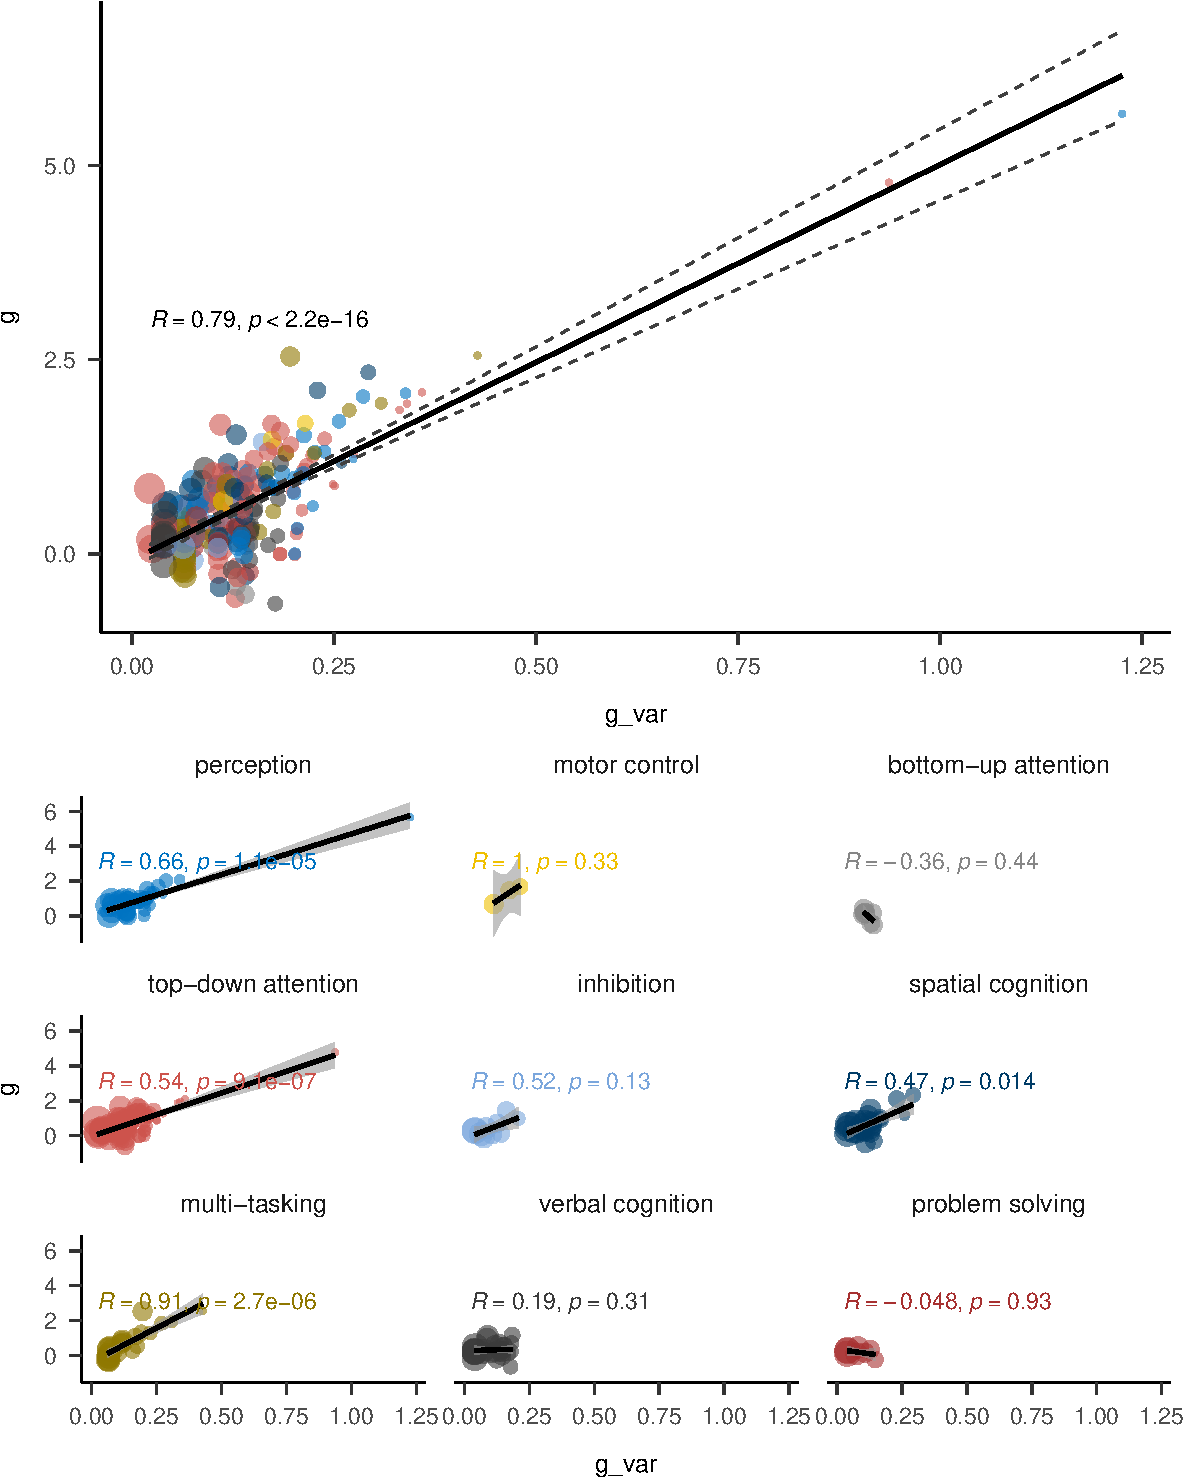
\includegraphics{MetaAnalysis_CrossSectional_files/figure-latex/unnamed-chunk-4-1.pdf}

\hypertarget{vs-2021}{%
\section{2018 vs 2021}\label{vs-2021}}

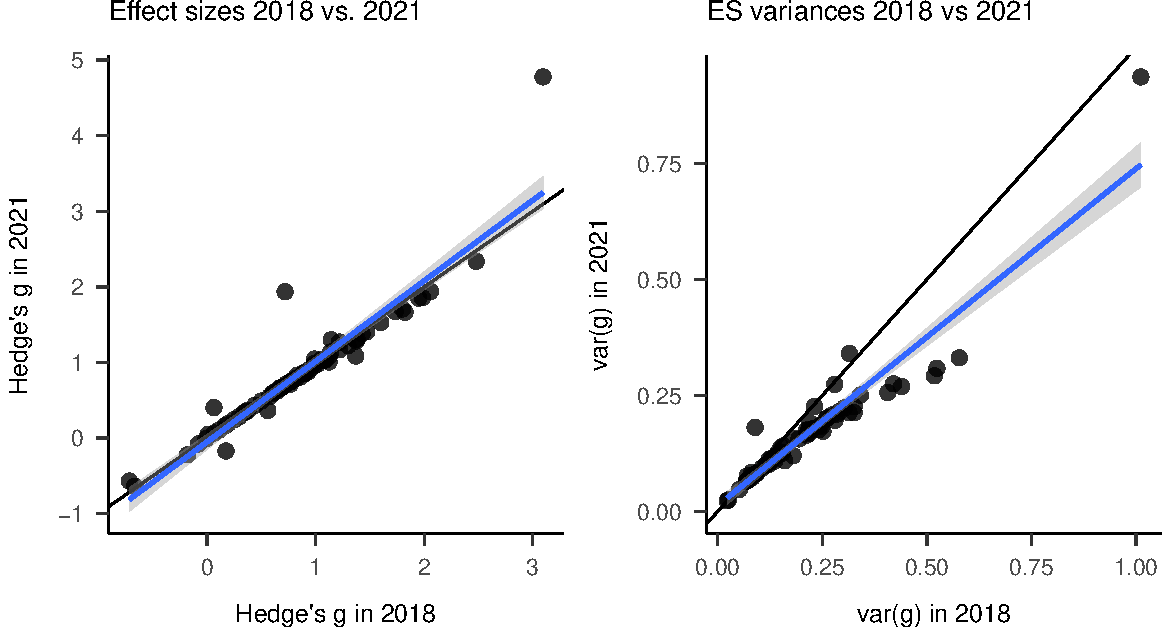
\includegraphics{MetaAnalysis_CrossSectional_files/figure-latex/esCompare-1.pdf}

\hypertarget{metaana}{%
\chapter{Meta-analysis}\label{metaana}}

\begin{quote}
TODO: improve code for moderator and pub bias (loop? function? check Pustejobsky's code)
\end{quote}

\textbf{Important Notes:}\\
- All analyses are done on the \emph{winsorized} dataset (i.e., extreme values replaced distribution boundaries)\\
- All clustering is done at the \emph{manuscript} level.\\
=\textgreater{} This can be changed! Let me know if we should chat about these points!

\hypertarget{overall-estimate}{%
\section{Overall estimate}\label{overall-estimate}}

We use a multilevel meta-analytic model with robust variance estimates (RVE)
for correlated and hierarchical effects (CHE) with small sample correction.\\
The default correlation is set to 0.8 (default in RVE), and we use
sensitivity analyses (see below) to test the impact of different values.
The model includes a random factor for Papers and one for each effect sizes nested
in papers.

\hypertarget{multilevel-model-without-rve}{%
\subsection{Multilevel model (without RVE)}\label{multilevel-model-without-rve}}

\begin{verbatim}
## 
## Multivariate Meta-Analysis Model (k = 224; method: REML)
## 
## Variance Components:
## 
##             estim    sqrt  nlvls  fixed       factor 
## sigma^2.1  0.0191  0.1382     73     no        Paper 
## sigma^2.2  0.1200  0.3464    224     no  Paper/ES_ID 
## 
## Test for Heterogeneity:
## Q(df = 223) = 1007.1261, p-val < .0001
## 
## Model Results:
## 
## estimate      se     tval   df    pval   ci.lb   ci.ub 
##   0.6227  0.0512  12.1651  223  <.0001  0.5218  0.7236  *** 
## 
## ---
## Signif. codes:  0 '***' 0.001 '**' 0.01 '*' 0.05 '.' 0.1 ' ' 1
\end{verbatim}

Note that this model reports model-based (not robust) standard errors.

The MLMA model reveals significant effect of AVG experience on cognition, with
AVGPs outperforming NVGPs on cognitive tasks.

\begin{itemize}
\item
  Overall estimate: \emph{g} = 0.623, \emph{p} = \textless.001
\item
  Residual heterogeneity is significant (\emph{QE}(223) = 1007.126,
  \emph{p} = \textless.001), suggesting possible moderating variables!
\end{itemize}

\hypertarget{che-model-multilevel-model-with-cluster-level-rve}{%
\subsection{CHE model: Multilevel model with cluster-level RVE}\label{che-model-multilevel-model-with-cluster-level-rve}}

This new model for Correlated and Hierarchical Effects (CHE) is based on recent work
from Pustejovsky \& Tipton (2021) as an extension of the range of RVE models.
The CHE model was shown to better capture the types of data structure that
occur in practice and --under some circumstances-- to improve the efficiency of
meta-regression estimates.

\begin{verbatim}
##     Coef. Estimate     SE t-stat d.f. p-val (Satt) Sig.
## 1 intrcpt    0.623 0.0513   12.1 59.6       <0.001  ***
\end{verbatim}

The cluster RVE is applied to adjust degrees of freedom and confidence intervals.\\
The CHE model usually gives smaller SE indicating improved precision.

\hypertarget{standard-rve-models-with-correlated-or-hierarchical-weights}{%
\subsection{Standard RVE models with correlated or hierarchical weights}\label{standard-rve-models-with-correlated-or-hierarchical-weights}}

For comparison with Bediou et al.~2018, we ran standard RVE models with correlated
and hierarchical weights.

\begin{verbatim}
## RVE: Correlated Effects Model with Small-Sample Corrections 
## 
## Model: es_win ~ 1 
## 
## Number of studies = 73 
## Number of outcomes = 224 (min = 1 , mean = 3.07 , median = 2 , max = 18 )
## Rho = 0.8 
## I.sq = 53.6 
## Tau.sq = 0.13 
## 
##                Estimate StdErr t-value  dfs P(|t|>) 95% CI.L 95% CI.U Sig
## 1 X.Intercept.    0.667 0.0513      13 67.9       0    0.565     0.77 ***
## ---
## Signif. codes: < .01 *** < .05 ** < .10 *
## ---
## Note: If df < 4, do not trust the results
\end{verbatim}

\begin{verbatim}
## RVE: Hierarchical Effects Model with Small-Sample Corrections 
## 
## Model: es_win ~ 1 
## 
## Number of clusters = 73 
## Number of outcomes = 224 (min = 1 , mean = 3.07 , median = 2 , max = 18 )
## Omega.sq = 0 
## Tau.sq = 0.11 
## 
##                Estimate StdErr t-value  dfs       P(|t|>) 95% CI.L 95% CI.U Sig
## 1 X.Intercept.    0.527 0.0614    8.59 27.2 0.00000000312    0.401    0.653 ***
## ---
## Signif. codes: < .01 *** < .05 ** < .10 *
## ---
## Note: If df < 4, do not trust the results
\end{verbatim}

\textbf{Sensitivity analysis}\\
We test impact of different values of rho (correlation among dependent ES's) on the
overall estimates using a standard RVE model with correlated weights.

\begin{verbatim}
## RVE: Correlated Effects Model with Small-Sample Corrections 
## Model: es_win ~ 1 
## 
## Sensitivity Analysis 
## 
##                           Rho = 0 Rho = 0.2 Rho = 0.4 Rho = 0.6 Rho = 0.8
##  X.Intercept. Coefficient 0.6673  0.6674    0.6674    0.6674    0.6675   
##               Std. Error  0.0513  0.0513    0.0513    0.0513    0.0513   
##  Tau.sq       Estimate    0.1291  0.1292    0.1293    0.1295    0.1296   
##  Rho = 1
##  0.6675 
##  0.0513 
##  0.1297
\end{verbatim}

\begin{itemize}
\item
  Overall estimate: \emph{g} = 0.667, \emph{p} = \textless.001
\item
  Residual heterogeneity is significant (\emph{QE} (223) = 1007.126,
  \emph{p} = \textless.001), suggesting possible moderating variables!
\end{itemize}

\hypertarget{univariate-meta-analysis-for-pub-bias}{%
\subsection{univariate meta-analysis (for pub bias)}\label{univariate-meta-analysis-for-pub-bias}}

We also ran univariate models to apply the more classical methods for
detection and correction of publication bias. Because univariate models assume
independent effect sizes, we first randomly selected one effect size per study (paper).

\begin{verbatim}
## 
## Random-Effects Model (k = 73; tau^2 estimator: REML)
## 
## tau^2 (estimated amount of total heterogeneity): 0.1214 (SE = 0.0408)
## tau (square root of estimated tau^2 value):      0.3485
## I^2 (total heterogeneity / total variability):   52.39%
## H^2 (total variability / sampling variability):  2.10
## 
## Test for Heterogeneity:
## Q(df = 72) = 151.0859, p-val < .0001
## 
## Model Results:
## 
## estimate      se     zval    pval   ci.lb   ci.ub 
##   0.6689  0.0587  11.3909  <.0001  0.5538  0.7840  *** 
## 
## ---
## Signif. codes:  0 '***' 0.001 '**' 0.01 '*' 0.05 '.' 0.1 ' ' 1
\end{verbatim}

\hypertarget{summary-of-overall-effects}{%
\subsection{Summary of overall effects}\label{summary-of-overall-effects}}

\begin{table}
\centering
\begin{tabular}{l|r|r|r|r|r|r|l}
\hline
Model & beta & SE & CI\_L & CI\_U & tstat & df & pSignif\\
\hline
RVE correlated & 0.667 & 0.051 & 0.565 & 0.770 & 13.01 & 67.9 & <.001\\
\hline
RVE hierarchical & 0.527 & 0.061 & 0.401 & 0.653 & 8.59 & 27.2 & <.001\\
\hline
\textbf{CHE} & \textbf{0.623} & \textbf{0.051} & \textbf{0.520} & \textbf{0.725} & \textbf{12.15} & \textbf{59.6} & \textbf{<.001}\\
\hline
univariate & 0.669 & 0.059 & 0.554 & 0.784 & 11.39 & 73.0 & <.001\\
\hline
\end{tabular}
\end{table}

Note. We pre-registered the CHE model as our primary model; other models are presented
to show sensitivity of our results to various meta-analytic models.

\hypertarget{moderator-analysis}{%
\section{Moderator analysis}\label{moderator-analysis}}

Moderator analysis is based on the multilevel model (i.e.~mlma \textbf{WITHOUT RVE}) because the
Wald\_test is not compatible with the CHE model (i.e., mlma with RVE)\ldots{}

Our model includes moderators:\\
- Cognitive domain (9 levels)\\
- DV type: speed, accuracy (\textbf{should we relabel as} \emph{performance} \textbf{measure\_ ?})\\
- Effect: main (e.g., overall performance), interaction (e.g., difference score)\\
- Recruitment: overt, covert

\hypertarget{compare-rve-che-and-sce-models}{%
\subsection{Compare RVE, CHE and SCE models}\label{compare-rve-che-and-sce-models}}

\begin{quote}
Notes:\\
- RVE = Robust Variance Estimate (effect sizes clustered by paper, correlated weights)\\
- CHE = Correlated Hierarchical Weights (random effects multilevel model with RVE)\\
- SCE = Subgroup Correlated Effects (alternative to running meta-analyses for each subgroup)\\
=\textgreater{} SCE RANDOM EFFECTS TO BE CHECKED BY MELISSA !
\end{quote}

This analysis focuses on cognitive domain (primary moderator) and controls for other (secondary) moderators. The magnitude of the obtained estimates depends on the choice of reference levels for secondary moderators.\\
The Wald Test of moderator effects test the relative differences between levels and is thus not sensitive to reference levels. However, to test if individual estimate differs from zero, we need to correct each estimate using the relative frequency of each moderator level in the dataset.

All models include the following moderators and reference levels:\\
- Cognitive domain: reference = perception\\
- DV type: reference = accuracy\\
- Effect type: reference = interaction\\
- Recruitment: reference = covert

Analyses of moderator effects are based on CHE model.\\
Exploratory analyses using Subgroup Correlated Effects are also presented.

\hypertarget{tests-of-moderator-effects-using-che-model}{%
\subsection{Tests of moderator effects (using CHE model)}\label{tests-of-moderator-effects-using-che-model}}

\begin{table}
\begin{tabular}{l|l|r|r|r|r|r}
\hline
moderator & test & Fstat & delta & df\_num & df\_denom & p\_val\\
\hline
Cognitive domain & HTZ & 0.575 & 1.000 & 1 & 1.18 & 0.570\\
\cline{1-7}
DV type & HTZ & 2.260 & 0.488 & 8 & 6.67 & 0.155\\
\cline{1-7}
Effect & HTZ & 0.021 & 1.000 & 1 & 21.36 & 0.885\\
\cline{1-7}
\cellcolor{gray}{\textcolor{white}{\textbf{Recruitment}}} & \cellcolor{gray}{\textcolor{white}{\textbf{HTZ}}} & \cellcolor{gray}{\textcolor{white}{\textbf{4.573}}} & \cellcolor{gray}{\textcolor{white}{\textbf{1.000}}} & \cellcolor{gray}{\textcolor{white}{\textbf{1}}} & \cellcolor{gray}{\textcolor{white}{\textbf{7.71}}} & \cellcolor{gray}{\textcolor{white}{\textbf{0.066}}}\\
\hline
\end{tabular}
\end{table}

\hypertarget{estimates-for-each-moderator-level-different-from-zero}{%
\subsection{Estimates for each moderator level (different from zero?)}\label{estimates-for-each-moderator-level-different-from-zero}}

Notes: Estimates with degrees of freedom under 4 should not be interpreted and are thus highlighted.

\begin{itemize}
\item
  None of the moderators showed significant moderating influence according to AHT-F test
  (using \emph{clubSandwich::Wald\_test}) on the multilevel model (i.e., \textbf{without RVE})
  except a marginal effect of recruitment.
\item
  AVGPs outperformed NVGPs in irrespective of cognitive domain, DV type, effect or recruitment method:

  \begin{itemize}
  \tightlist
  \item
    Cognitive domain: stronger effects for perception and multitasking, followed by top-down attention,
    spatial cognition and inhibition, and then verbal cognition. Marginal effect for problem solving and
    unreliable estimates (low df) for motor control and bottom-up attention.\\
  \item
    DV type: significant effects on speed and accuracy.\\
  \item
    Effect: significant group differences for both overall (main effect) performance measures and
    difference scores (interactions).\\
  \item
    Significant effect in both overtly and covertly recruited participants, with numerically larger effect
    for overt vs.~covert.
  \end{itemize}
\item
  Residual heterogeneity is still significant (\emph{QE}(212) = 915.77,
  \emph{p} = ), suggesting additional moderating variables may be involved !
  =\textgreater{} Additional analyses are needed to understand where this comes from:

  \begin{itemize}
  \tightlist
  \item
    publication bias / small study effect (adding variance or sda to moderator models?)\\
  \item
    lab / joint publication group\\
  \item
    single moderator models
  \end{itemize}
\end{itemize}

\hypertarget{publication-bias}{%
\section{Publication bias}\label{publication-bias}}

Numerous techniques exist for detecting and correcting publication bias.
While methods for detecting publication bias (or small study effects) have
improved largely over the past decades, it is not the case of correction methods
such that estimating a unbiased (or publication-bias-corrected) estimate remains a challenge.
The numerous methods available to date provide very heterogeneous estimates and will thus
be reported in the form of sensitivity analysis as as recently recommended by
Mathur \& VanderWeele (2020).

Detection of publication bias was done for both:\\
- The overall effect (intercept only model) and\\
- The full model including all moderators

Our main publication bias detection approach is based on Egger's regression test
with a modified precision covariate (Pustejovsky \& Rodgers, 2019).

In addition, we use a number of additional methods to estimate the adjusted effect,
because the estimates obtained from Eggers's test (and PET-PEESE) are known to be
unreliable.\\
The best methods for estimating the publication bias (or small-study) adjusted effect
is based on the 3-parameter model selection (see below).

\hypertarget{contour-enhanced-funnel-plots}{%
\subsection{(contour-enhanced) Funnel plots}\label{contour-enhanced-funnel-plots}}

Funnel plots are based on multilevel models \emph{without RVE}, first for overall effect (i.e., intercept only)
and then for the full model (i.e., with all moderators).\\
In order to use trim and fill, we also conducted a univariate model using one randomly sampled estimate
from each cluster.\\
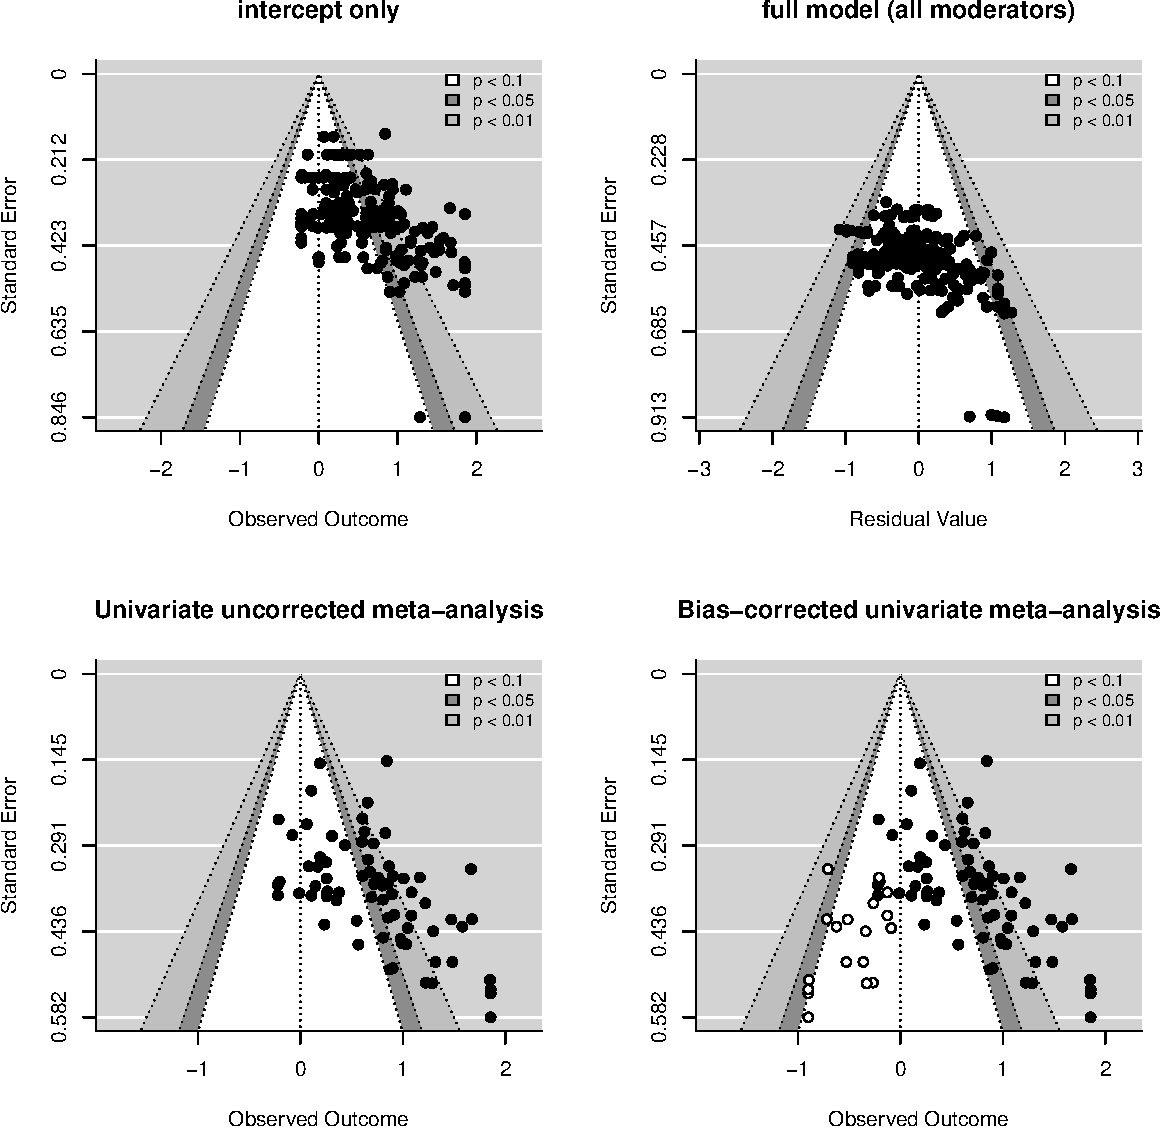
\includegraphics{MetaAnalysis_CrossSectional_files/figure-latex/unnamed-chunk-5-1.pdf}

\hypertarget{significance-funnel-plot-mathur-vanderweele-2020}{%
\subsection{Significance funnel plot (Mathur \& VanderWeele, 2020)}\label{significance-funnel-plot-mathur-vanderweele-2020}}

This new type of graphical illustration was introduced recently as an alternative to funnel plots.\\
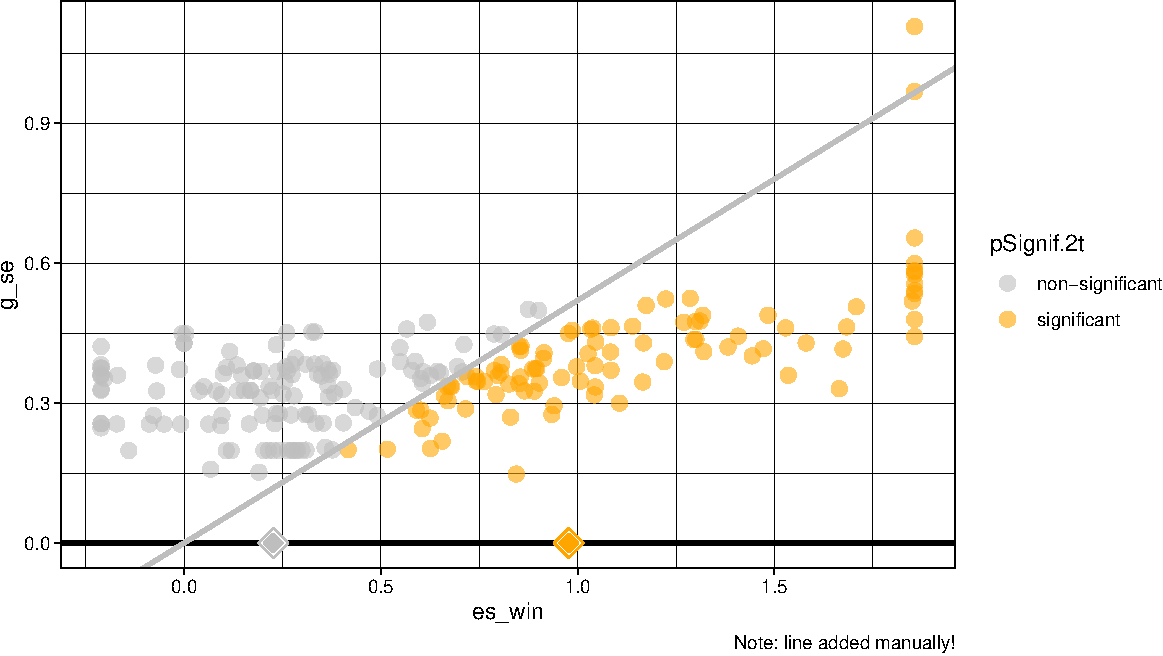
\includegraphics{MetaAnalysis_CrossSectional_files/figure-latex/pb_estimates-1.pdf}
Note: the line was drawn manually (i.e., no classification applied) with\\
intercept = 0 and slope = 0.52.

Non-affirmative studies have smaller point estimates than affirmative studies,
suggesting that results may be sensitive to publication bias.

\hypertarget{eggers-regression-with-modified-precision-covariate}{%
\subsection{Egger's regression with modified precision covariate}\label{eggers-regression-with-modified-precision-covariate}}

This method is based on work from Pustejovsky and Rodgers (2018), and Rodgers \& Pustejovsky (2020).\\
The new (Egger's sandwich) test has been shown to maintain type I error (unlike the inflated type I errors
commonly reported with other methods).

\begin{quote}
Quote from Pustejovsky \& Rodgers 2020, page 36:\\
\emph{``the Egger Sandwich is an acceptable, valid test for meta-analysis, but it must be interpreted
with caution both because it has limited power to detect funnel plot asymmetry
and because, in practice, such asymmetry may have other causes besides selective reporting.''}\\
\emph{``The Funnel Plot Test with MLMA maintains Type I error across nearly all conditions,
and like the Egger Sandwich, it lacks power to detect funnel plot asymmetry.''}
\end{quote}

We ran both Egger's Sandwich and Egger's MLMA models on both overall effect (intercept only)
and full model with all moderators.

\begin{tabular}{l|l|l|r|r|r|r|r|r|r}
\hline
method & model & term & b & se & t & dfs & p & ci.lb & ci.ub\\
\hline
\cellcolor{yellow}{Egger CHE (MLMA + RVE)} & \cellcolor{yellow}{NULL} & \cellcolor{yellow}{intrcpt} & \cellcolor{yellow}{-0.043} & \cellcolor{yellow}{0.182} & \cellcolor{yellow}{-0.234} & \cellcolor{yellow}{13.4} & \cellcolor{yellow}{0.819} & \cellcolor{yellow}{-0.434} & \cellcolor{yellow}{0.349}\\
\cline{1-10}
\cellcolor{yellow}{\textbf{Egger CHE (MLMA + RVE)}} & \cellcolor{yellow}{\textbf{NULL}} & \cellcolor{yellow}{\textbf{sda}} & \cellcolor{yellow}{\textbf{1.897}} & \cellcolor{yellow}{\textbf{0.533}} & \cellcolor{yellow}{\textbf{3.560}} & \cellcolor{yellow}{\textbf{18.3}} & \cellcolor{yellow}{\textbf{0.002}} & \cellcolor{yellow}{\textbf{0.779}} & \cellcolor{yellow}{\textbf{3.014}}\\
\cline{1-10}
\cellcolor{yellow}{Egger CHE (MLMA + RVE)} & \cellcolor{yellow}{FULL} & \cellcolor{yellow}{intrcpt} & \cellcolor{yellow}{0.025} & \cellcolor{yellow}{0.200} & \cellcolor{yellow}{0.125} & \cellcolor{yellow}{19.5} & \cellcolor{yellow}{0.902} & \cellcolor{yellow}{-0.394} & \cellcolor{yellow}{0.444}\\
\cline{1-10}
\cellcolor{yellow}{\textbf{Egger CHE (MLMA + RVE)}} & \cellcolor{yellow}{\textbf{FULL}} & \cellcolor{yellow}{\textbf{sda}} & \cellcolor{yellow}{\textbf{1.793}} & \cellcolor{yellow}{\textbf{0.648}} & \cellcolor{yellow}{\textbf{2.767}} & \cellcolor{yellow}{\textbf{22.3}} & \cellcolor{yellow}{\textbf{0.011}} & \cellcolor{yellow}{\textbf{0.450}} & \cellcolor{yellow}{\textbf{3.136}}\\
\cline{1-10}
Egger Sandwich (RVE) & NULL & intrcpt & -0.028 & 0.258 & -0.109 & 12.0 & 0.915 & -0.591 & 0.535\\
\cline{1-10}
\textbf{Egger Sandwich (RVE)} & \textbf{NULL} & \textbf{sda} & \textbf{2.043} & \textbf{0.729} & \textbf{2.803} & \textbf{14.9} & \textbf{0.013} & \textbf{0.488} & \textbf{3.597}\\
\cline{1-10}
Egger Sandwich (RVE) & FULL & intrcpt & 0.156 & 0.243 & 0.640 & 23.5 & 0.528 & -0.347 & 0.658\\
\cline{1-10}
\textbf{Egger Sandwich (RVE)} & \textbf{FULL} & \textbf{sda} & \textbf{1.906} & \textbf{0.732} & \textbf{2.605} & \textbf{15.0} & \textbf{0.020} & \textbf{0.346} & \textbf{3.466}\\
\hline
\end{tabular}

\emph{note: p values are based on one-sided test as the Egger's Sandwich test is done to look}
\emph{at the slope of missing negative effects on the left side of the funnel plot.}

\textbf{Summary:}

\begin{itemize}
\tightlist
\item
  The slope (sda) is significant indicating significant publication bias.\\
\item
  The Intercept is not a reliable estimate of the bias-corrected effect (but shows how adding
  publication bias / small study affects the estimate).\\
\item
  The other estimates can be ignored too as they are sensitive to choice of reference levels!\\
\item
  Surprisingly, heterogeneity is still highly significant, even when including all moderators!\\
  =\textgreater{} subgroup analyses?\\
  =\textgreater{} moderators lab / joint publication group?\\
  =\textgreater{} other suggestions\ldots?
\end{itemize}

\hypertarget{pet-peese}{%
\subsection{PET-PEESE}\label{pet-peese}}

Here, we applied PET and PEESE to our multilevel model with cluster robust variance (CHE model).\\
For PEESE, we used the modified precision estimate because it increases precision.

For comparison with Bediou et al., 2018, we also applied PET and PEESE to standard RVE models
hierarchical weights and obtained similar results. In addition to the hierarchical weights
used in Bediou et al.~2018, we also use correlated weights because they have been shown to
perform significantly better in most situations.

Again, we ran the analysis both on the overall effect (i.e., intercept only) model and on the full model
with all moderators.

Following Stanley \& Doucouliagos 2013, we use the conditional PET-PEESE estimate as follows:\\
- If PET estimate is significant, we use PEESE estimate.\\
- If PET is NS, then we use PET estimate.

\begin{quote}
Note that this approach has been extensively criticized for its limitations,
including by the authors themselves.\\
Melissa recommended to drop PET-PEESE entirely because it is known to inflate
type I error and has been consistently outperformed by the new precision estimate
used by Egger Sandwich.
I left them for comparison with Bediou et al.~2018.
\end{quote}

\begin{tabular}{l|l|l|r|r|r|r|r|r|r}
\hline
method & model & term & b & se & t & dfs & p & ci.lb & ci.ub\\
\hline
 & NULL & intrcpt & -0.385 & 0.170 & -2.262 & 6.26 & 0.063 & -0.797 & 0.027\\
\cline{2-10}
\multirow[t]{-2}{*}{\raggedright\arraybackslash PET (RVE hier)} & FULL & intrcpt & -0.291 & 0.163 & -1.789 & 24.09 & 0.086 & -0.627 & 0.045\\
\cline{1-10}
 & NULL & intrcpt & -0.272 & 0.218 & -1.247 & 14.73 & 0.232 & -0.738 & 0.194\\
\cline{2-10}
\multirow[t]{-2}{*}{\raggedright\arraybackslash PET (RVE corr)} & FULL & intrcpt & -0.085 & 0.185 & -0.458 & 23.79 & 0.651 & -0.467 & 0.297\\
\cline{1-10}
 & \textbf{NULL} & \textbf{intrcpt} & \textbf{-0.498} & \textbf{0.203} & \textbf{-2.454} & \textbf{15.87} & \textbf{0.026} & \textbf{-0.928} & \textbf{-0.067}\\
\cline{2-10}
\multirow[t]{-2}{*}{\raggedright\arraybackslash \textbf{PET (CHE)}} & \textbf{FULL} & \textbf{intrcpt} & \textbf{-0.411} & \textbf{0.195} & \textbf{-2.108} & \textbf{20.56} & \textbf{0.048} & \textbf{-0.818} & \textbf{-0.005}\\
\cline{1-10}
 & NULL & intrcpt & 0.085 & 0.096 & 0.885 & 6.68 & 0.407 & -0.144 & 0.314\\
\cline{2-10}
\multirow[t]{-2}{*}{\raggedright\arraybackslash PEESE (RVE hier)} & FULL & intrcpt & 0.211 & 0.133 & 1.589 & 22.09 & 0.126 & -0.064 & 0.487\\
\cline{1-10}
 & \textbf{NULL} & \textbf{slope} & \textbf{3.676} & \textbf{0.780} & \textbf{4.714} & \textbf{7.42} & \textbf{0.002} & \textbf{1.853} & \textbf{5.498}\\
\cline{2-10}
\multirow[t]{-2}{*}{\raggedright\arraybackslash \textbf{PEESE (RVE hier)}} & \textbf{FULL} & \textbf{slope} & \textbf{3.673} & \textbf{1.011} & \textbf{3.634} & \textbf{7.00} & \textbf{0.008} & \textbf{1.283} & \textbf{6.063}\\
\cline{1-10}
PEESE (RVE corr) & NULL & intrcpt & 0.220 & 0.128 & 1.719 & 12.71 & 0.110 & -0.057 & 0.496\\
\cline{1-10}
 & \textbf{FULL} & \textbf{intrcpt} & \textbf{0.367} & \textbf{0.148} & \textbf{2.478} & \textbf{18.24} & \textbf{0.023} & \textbf{0.056} & \textbf{0.677}\\
\cline{2-10}
 & \textbf{NULL} & \textbf{slope} & \textbf{3.390} & \textbf{0.928} & \textbf{3.654} & \textbf{7.82} & \textbf{0.007} & \textbf{1.242} & \textbf{5.539}\\
\cline{2-10}
\multirow[t]{-3}{*}{\raggedright\arraybackslash \textbf{PEESE (RVE corr)}} & \textbf{FULL} & \textbf{slope} & \textbf{3.145} & \textbf{0.900} & \textbf{3.494} & \textbf{7.69} & \textbf{0.009} & \textbf{1.055} & \textbf{5.235}\\
\cline{1-10}
 & NULL & intrcpt & 0.175 & 0.192 & 0.911 & 10.41 & 0.383 & -0.251 & 0.601\\
\cline{2-10}
 & FULL & intrcpt & 0.206 & 0.167 & 1.236 & 18.45 & 0.232 & -0.144 & 0.556\\
\cline{2-10}
 & NULL & slope & 3.417 & 1.506 & 2.268 & 5.75 & 0.066 & -0.309 & 7.142\\
\cline{2-10}
\multirow[t]{-4}{*}{\raggedright\arraybackslash PEESE (CHE)} & FULL & slope & 3.318 & 1.553 & 2.136 & 5.63 & 0.080 & -0.544 & 7.179\\
\hline
\end{tabular}

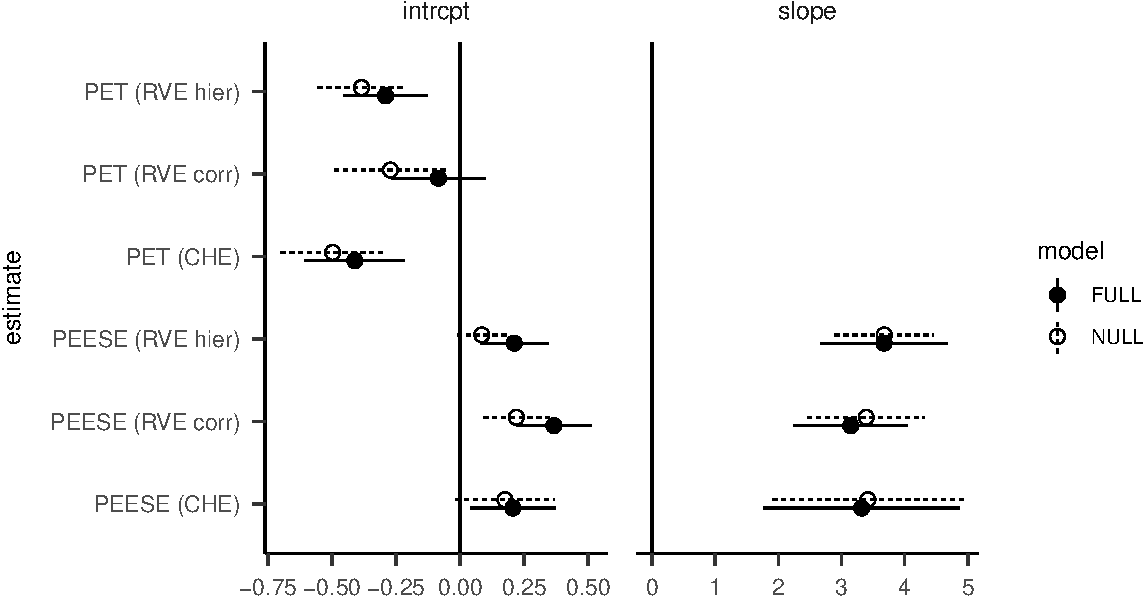
\includegraphics{MetaAnalysis_CrossSectional_files/figure-latex/peese-1.pdf}

\hypertarget{bootstraped-estimates-for-univariate-analyses}{%
\subsection{Bootstraped estimates for univariate analyses}\label{bootstraped-estimates-for-univariate-analyses}}

Trim and fill, p-uniform and 3-PSM work only with independent effect sizes.\\
In order to run these analyses, we thus randomly picked one effect size per study (i.e.~paper).\\
To verify that this random sampling does not introduce bias, we first checked the distribution of
the overall effect obtained from 1000 bootstrapped samples of one effect size per paper.

\begin{verbatim}
##      term     b     se ci.lb ci.ub
## 1 intrcpt 0.494 0.0307 0.433 0.558
\end{verbatim}

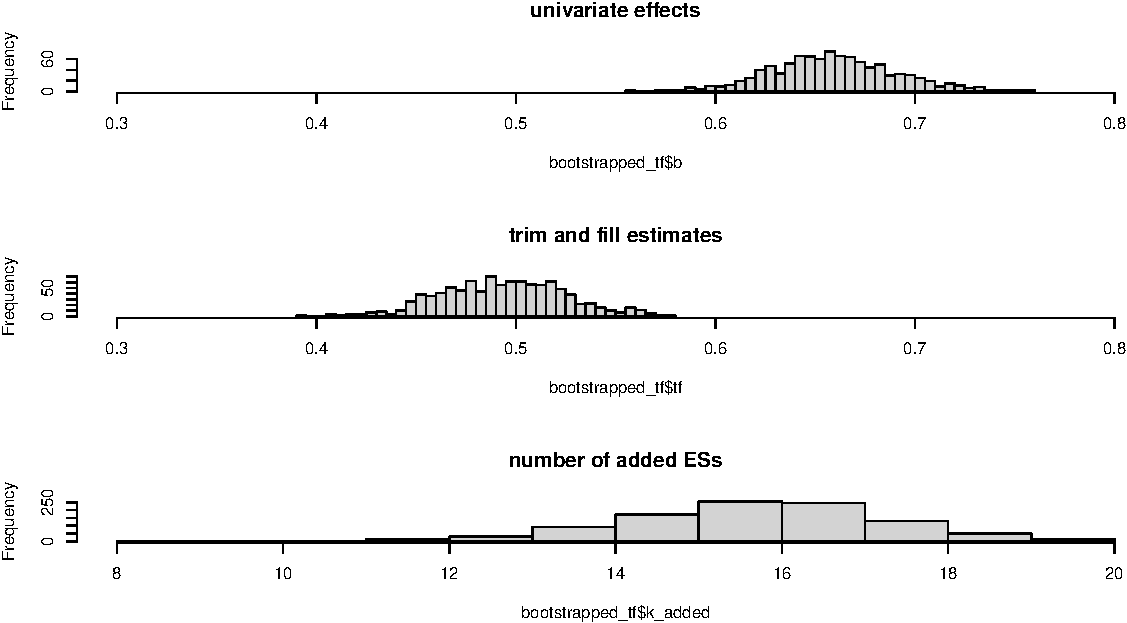
\includegraphics{MetaAnalysis_CrossSectional_files/figure-latex/bootstrap_tf-1.pdf}
The univariate meta-analysis of 73 randomly selected independent effect sizes revealed
an average overall effect of \emph{mean g} = 0.659
(\emph{SD} = 0.031)

\hypertarget{bootstrapped-trim-and-fill-duval-tweedie-2001}{%
\subsection{Bootstrapped trim and fill (Duval \& Tweedie, 2001)}\label{bootstrapped-trim-and-fill-duval-tweedie-2001}}

Across the 1000 bootstrapped samples, trim and fill analysis imputed between
8 and 20 additional effects
on the left side of the funnel plot (median = 16), in order
to correct for its asymmetry.

These additional studies decreased the overall estimate to a mean of \emph{g} = 0.494
(\emph{SD} = 0.031), but did not alter significance \emph{all p's} \textless{} .001).

\hypertarget{p-uniform-van-assen-van-aert-wicherts-2015}{%
\subsection{P-Uniform (van Assen, van Aert \& Wicherts, 2015)}\label{p-uniform-van-assen-van-aert-wicherts-2015}}

p-uniform is fundamentally similar to a p-curve that estimates the true effect
using only significant effects. This method is not without limitations; it tends
to overestimate effect sizes when heterogeneity is moderate to large, and is
insensitive to p-values that are close to significance, or in the presence of
p-hacking (Van Aerts, Wicherts \& van Assen, 2016).

\begin{verbatim}
##      term     b     se ci.lb ci.ub
## 1 intrcpt 0.706 0.0338 0.637 0.772
\end{verbatim}

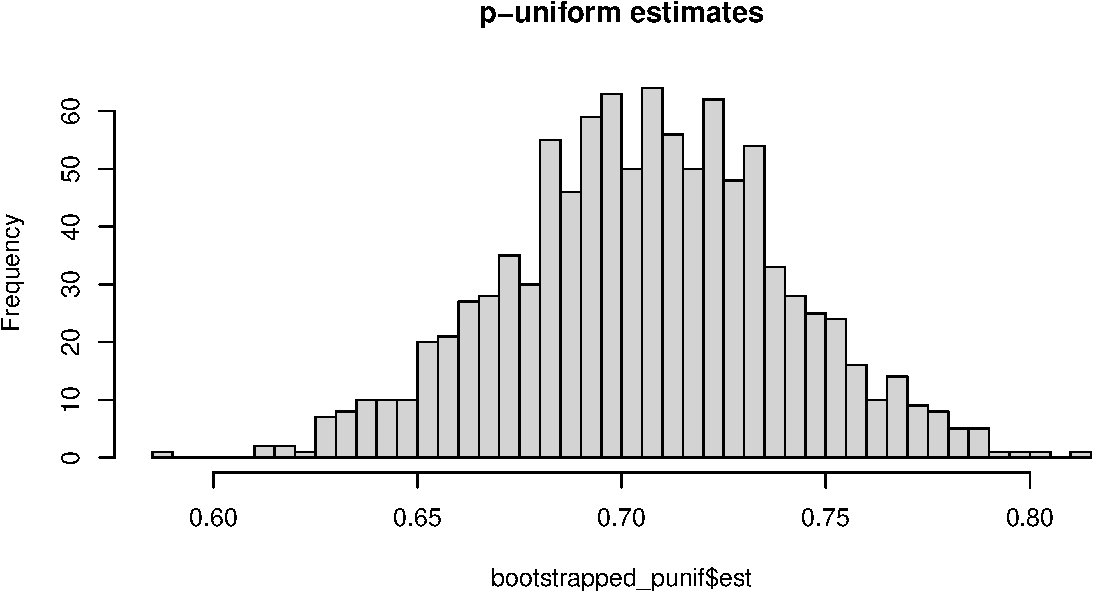
\includegraphics{MetaAnalysis_CrossSectional_files/figure-latex/punif-1.pdf}
Studies with lower p values are observed less often than expected, whereas studies with high p values
are more frequent than expected. Yet, the test of publication bias is not significant (pval = 1).

\hypertarget{parameter-selection-model-3psm-hedges-vevea-1996.}{%
\subsection{3-Parameter Selection Model (3PSM, Hedges \& Vevea 1996).}\label{parameter-selection-model-3psm-hedges-vevea-1996.}}

Selection models are a general class of models that attempt to model the process by which the studies included in a meta-analysis may have been influenced by some form of publication bias. If a particular selection model is an adequate approximation for the underlying selection process, then the model provides estimates of the parameters of interest (e.g., the average true outcome and the amount of heterogeneity in the true outcomes) that are `corrected' for this selection process (i.e., they are estimates of the parameters in the population of studies before any selection has taken place).

\textbf{PSM Using selmodel function from metafor }\\
This function allows to test different models.\\
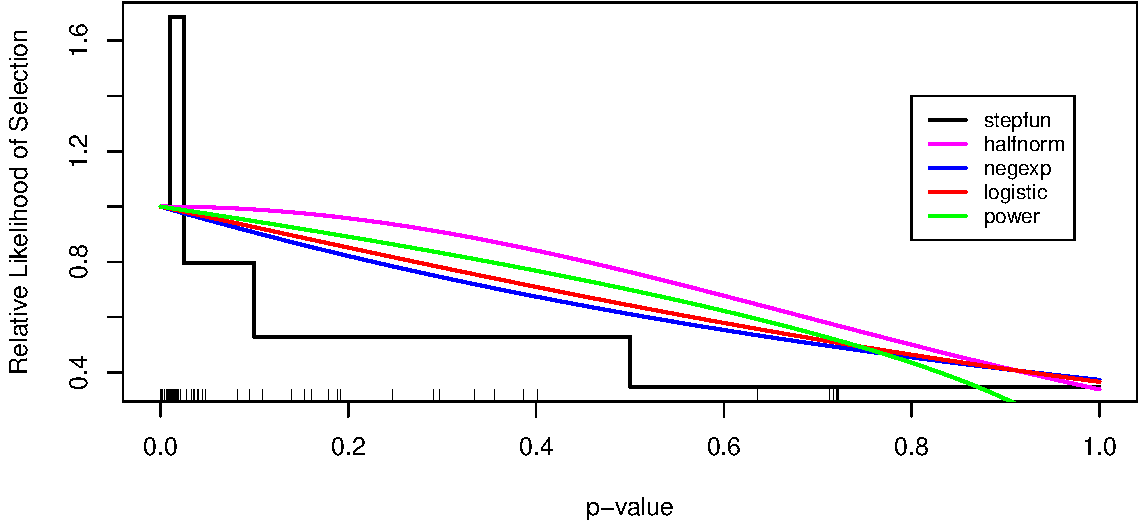
\includegraphics{MetaAnalysis_CrossSectional_files/figure-latex/4-PSM-1.pdf}
Colours show different (model-based) selective reporting biases:\\
- Negexpm and logistic selection give identical results.\\
- Step, halfnorm and Power give different results.

\textbf{3-PSM Using weightfunc from weightr }\\
Here we focus on the 3-PSM approach, which models publication bias with 3-parameters.
The first one represents how much less likely a non-significant result is to be published
than a significant result. The other two parameters represent the estimated bias-adjusted
mean effect and the estimated heterogeneity of the effects.

Below we plot the distribution of estimates corrected for publication bias that are
obtained from 100 bootstrapped samples with different thresholds for selective reporting
ranging from 0.1 to 0.001.\\
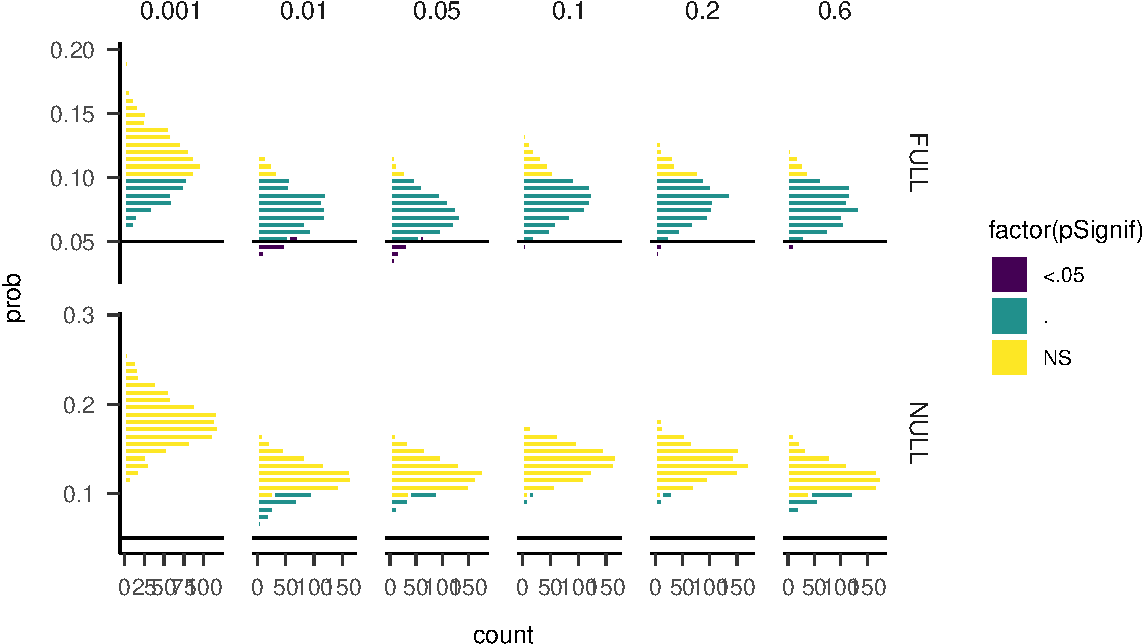
\includegraphics{MetaAnalysis_CrossSectional_files/figure-latex/3-PSM-1.pdf} 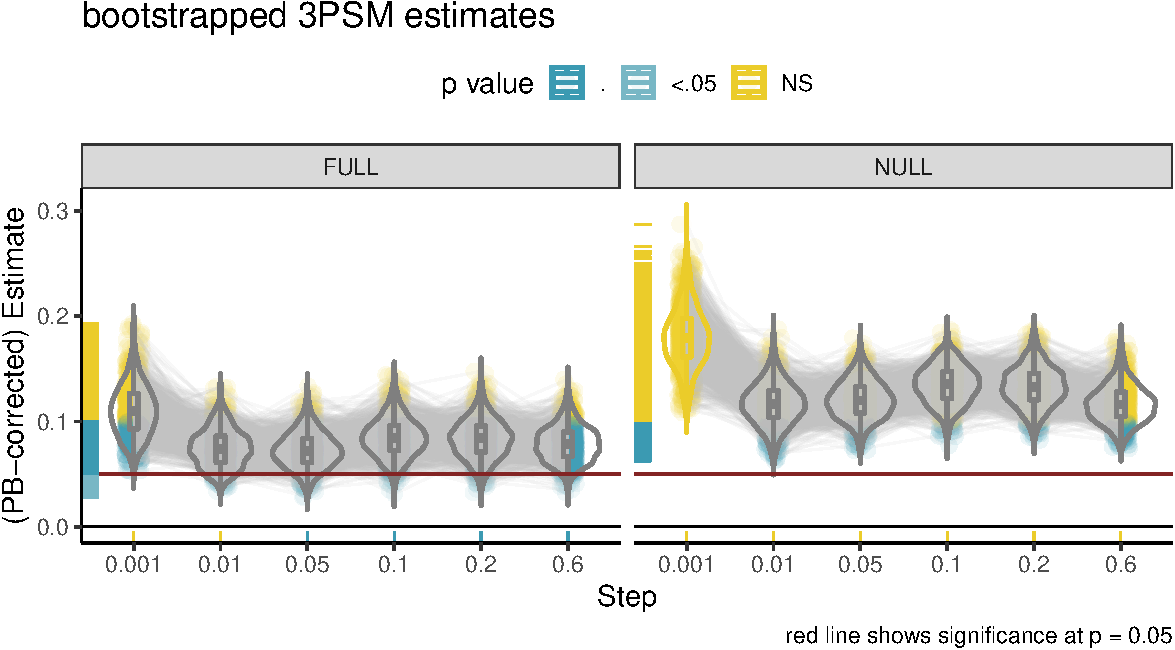
\includegraphics{MetaAnalysis_CrossSectional_files/figure-latex/3-PSM-2.pdf}

\hypertarget{publication-bias-corrected-estimates-obtained-from-regression-methods}{%
\subsection{Publication-bias-corrected estimates obtained from regression methods}\label{publication-bias-corrected-estimates-obtained-from-regression-methods}}

\begin{tabular}{l|l|l|r|r|r|r|r|r|r|l}
\hline
method & model & term & b & se & ci.lb & ci.ub & t & dfs & p & pSignif\\
\hline
 & \cellcolor[HTML]{85C1E9}{\textcolor{gray}{NULL}} & \cellcolor[HTML]{85C1E9}{\textcolor{gray}{intrcpt}} & \cellcolor[HTML]{85C1E9}{\textcolor{gray}{-0.498}} & \cellcolor[HTML]{85C1E9}{\textcolor{gray}{0.203}} & \cellcolor[HTML]{85C1E9}{\textcolor{gray}{-0.928}} & \cellcolor[HTML]{85C1E9}{\textcolor{gray}{-0.067}} & \cellcolor[HTML]{85C1E9}{\textcolor{gray}{-2.454}} & \cellcolor[HTML]{85C1E9}{\textcolor{gray}{15.87}} & \cellcolor[HTML]{85C1E9}{\textcolor{gray}{0.026}} & \cellcolor[HTML]{85C1E9}{\textcolor{gray}{<.05}}\\
\cline{2-11}
\multirow[t]{-2}{*}{\raggedright\arraybackslash \cellcolor[HTML]{85C1E9}{\textcolor{gray}{PET (CHE)}}} & \cellcolor[HTML]{85C1E9}{\textcolor{gray}{FULL}} & \cellcolor[HTML]{85C1E9}{\textcolor{gray}{intrcpt}} & \cellcolor[HTML]{85C1E9}{\textcolor{gray}{-0.411}} & \cellcolor[HTML]{85C1E9}{\textcolor{gray}{0.195}} & \cellcolor[HTML]{85C1E9}{\textcolor{gray}{-0.818}} & \cellcolor[HTML]{85C1E9}{\textcolor{gray}{-0.005}} & \cellcolor[HTML]{85C1E9}{\textcolor{gray}{-2.108}} & \cellcolor[HTML]{85C1E9}{\textcolor{gray}{20.56}} & \cellcolor[HTML]{85C1E9}{\textcolor{gray}{0.048}} & \cellcolor[HTML]{85C1E9}{\textcolor{gray}{<.05}}\\
\cline{1-11}
\textcolor{black}{\em{\textbf{\cellcolor[HTML]{85C1E9}{PET (RVE hier)}}}} & \textcolor{black}{\em{\textbf{\cellcolor[HTML]{85C1E9}{NULL}}}} & \textcolor{black}{\em{\textbf{\cellcolor[HTML]{85C1E9}{intrcpt}}}} & \textcolor{black}{\em{\textbf{\cellcolor[HTML]{85C1E9}{-0.385}}}} & \textcolor{black}{\em{\textbf{\cellcolor[HTML]{85C1E9}{0.170}}}} & \textcolor{black}{\em{\textbf{\cellcolor[HTML]{85C1E9}{-0.797}}}} & \textcolor{black}{\em{\textbf{\cellcolor[HTML]{85C1E9}{0.027}}}} & \textcolor{black}{\em{\textbf{\cellcolor[HTML]{85C1E9}{-2.262}}}} & \textcolor{black}{\em{\textbf{\cellcolor[HTML]{85C1E9}{6.26}}}} & \textcolor{black}{\em{\textbf{\cellcolor[HTML]{85C1E9}{0.063}}}} & \textcolor{black}{\em{\textbf{\cellcolor[HTML]{85C1E9}{.}}}}\\
\cline{1-11}
\cellcolor[HTML]{85C1E9}{\textcolor{gray}{PET (RVE hier)}} & \cellcolor[HTML]{85C1E9}{\textcolor{gray}{FULL}} & \cellcolor[HTML]{85C1E9}{\textcolor{gray}{intrcpt}} & \cellcolor[HTML]{85C1E9}{\textcolor{gray}{-0.291}} & \cellcolor[HTML]{85C1E9}{\textcolor{gray}{0.163}} & \cellcolor[HTML]{85C1E9}{\textcolor{gray}{-0.627}} & \cellcolor[HTML]{85C1E9}{\textcolor{gray}{0.045}} & \cellcolor[HTML]{85C1E9}{\textcolor{gray}{-1.789}} & \cellcolor[HTML]{85C1E9}{\textcolor{gray}{24.09}} & \cellcolor[HTML]{85C1E9}{\textcolor{gray}{0.086}} & \cellcolor[HTML]{85C1E9}{\textcolor{gray}{.}}\\
\cline{1-11}
 & \cellcolor[HTML]{85C1E9}{\textcolor{gray}{NULL}} & \cellcolor[HTML]{85C1E9}{\textcolor{gray}{intrcpt}} & \cellcolor[HTML]{85C1E9}{\textcolor{gray}{-0.272}} & \cellcolor[HTML]{85C1E9}{\textcolor{gray}{0.218}} & \cellcolor[HTML]{85C1E9}{\textcolor{gray}{-0.738}} & \cellcolor[HTML]{85C1E9}{\textcolor{gray}{0.194}} & \cellcolor[HTML]{85C1E9}{\textcolor{gray}{-1.247}} & \cellcolor[HTML]{85C1E9}{\textcolor{gray}{14.73}} & \cellcolor[HTML]{85C1E9}{\textcolor{gray}{0.232}} & \cellcolor[HTML]{85C1E9}{\textcolor{gray}{}}\\
\cline{2-11}
\multirow[t]{-2}{*}{\raggedright\arraybackslash \cellcolor[HTML]{85C1E9}{\textcolor{gray}{PET (RVE corr)}}} & \cellcolor[HTML]{85C1E9}{\textcolor{gray}{FULL}} & \cellcolor[HTML]{85C1E9}{\textcolor{gray}{intrcpt}} & \cellcolor[HTML]{85C1E9}{\textcolor{gray}{-0.085}} & \cellcolor[HTML]{85C1E9}{\textcolor{gray}{0.185}} & \cellcolor[HTML]{85C1E9}{\textcolor{gray}{-0.467}} & \cellcolor[HTML]{85C1E9}{\textcolor{gray}{0.297}} & \cellcolor[HTML]{85C1E9}{\textcolor{gray}{-0.458}} & \cellcolor[HTML]{85C1E9}{\textcolor{gray}{23.79}} & \cellcolor[HTML]{85C1E9}{\textcolor{gray}{0.651}} & \cellcolor[HTML]{85C1E9}{\textcolor{gray}{}}\\
\cline{1-11}
\cellcolor[HTML]{85C1E9}{\textcolor{gray}{Egger CHE (MLMA + RVE)}} & \cellcolor[HTML]{85C1E9}{\textcolor{gray}{NULL}} & \cellcolor[HTML]{85C1E9}{\textcolor{gray}{intrcpt}} & \cellcolor[HTML]{85C1E9}{\textcolor{gray}{-0.043}} & \cellcolor[HTML]{85C1E9}{\textcolor{gray}{0.182}} & \cellcolor[HTML]{85C1E9}{\textcolor{gray}{-0.434}} & \cellcolor[HTML]{85C1E9}{\textcolor{gray}{0.349}} & \cellcolor[HTML]{85C1E9}{\textcolor{gray}{-0.234}} & \cellcolor[HTML]{85C1E9}{\textcolor{gray}{13.35}} & \cellcolor[HTML]{85C1E9}{\textcolor{gray}{0.819}} & \cellcolor[HTML]{85C1E9}{\textcolor{gray}{}}\\
\cline{1-11}
\textcolor{black}{\em{\textbf{\cellcolor[HTML]{ABEBC6}{Egger Sandwich (RVE)}}}} & \textcolor{black}{\em{\textbf{\cellcolor[HTML]{ABEBC6}{NULL}}}} & \textcolor{black}{\em{\textbf{\cellcolor[HTML]{ABEBC6}{intrcpt}}}} & \textcolor{black}{\em{\textbf{\cellcolor[HTML]{ABEBC6}{-0.028}}}} & \textcolor{black}{\em{\textbf{\cellcolor[HTML]{ABEBC6}{0.258}}}} & \textcolor{black}{\em{\textbf{\cellcolor[HTML]{ABEBC6}{-0.591}}}} & \textcolor{black}{\em{\textbf{\cellcolor[HTML]{ABEBC6}{0.535}}}} & \textcolor{black}{\em{\textbf{\cellcolor[HTML]{ABEBC6}{-0.109}}}} & \textcolor{black}{\em{\textbf{\cellcolor[HTML]{ABEBC6}{12.00}}}} & \textcolor{black}{\em{\textbf{\cellcolor[HTML]{ABEBC6}{0.915}}}} & \textcolor{black}{\em{\textbf{\cellcolor[HTML]{ABEBC6}{}}}}\\
\cline{1-11}
\cellcolor[HTML]{ABEBC6}{\textcolor{gray}{Egger CHE (MLMA + RVE)}} & \cellcolor[HTML]{ABEBC6}{\textcolor{gray}{FULL}} & \cellcolor[HTML]{ABEBC6}{\textcolor{gray}{intrcpt}} & \cellcolor[HTML]{ABEBC6}{\textcolor{gray}{0.025}} & \cellcolor[HTML]{ABEBC6}{\textcolor{gray}{0.200}} & \cellcolor[HTML]{ABEBC6}{\textcolor{gray}{-0.394}} & \cellcolor[HTML]{ABEBC6}{\textcolor{gray}{0.444}} & \cellcolor[HTML]{ABEBC6}{\textcolor{gray}{0.125}} & \cellcolor[HTML]{ABEBC6}{\textcolor{gray}{19.51}} & \cellcolor[HTML]{ABEBC6}{\textcolor{gray}{0.902}} & \cellcolor[HTML]{ABEBC6}{\textcolor{gray}{}}\\
\cline{1-11}
\textcolor{black}{\em{\textbf{\cellcolor[HTML]{ABEBC6}{3-PSM}}}} & \textcolor{black}{\em{\textbf{\cellcolor[HTML]{ABEBC6}{FULL}}}} & \textcolor{black}{\em{\textbf{\cellcolor[HTML]{ABEBC6}{intrcpt}}}} & \textcolor{black}{\em{\textbf{\cellcolor[HTML]{ABEBC6}{0.079}}}} & \textcolor{black}{\em{\textbf{\cellcolor[HTML]{ABEBC6}{0.024}}}} & \textcolor{black}{\em{\textbf{\cellcolor[HTML]{ABEBC6}{0.040}}}} & \textcolor{black}{\em{\textbf{\cellcolor[HTML]{ABEBC6}{0.136}}}} & \textcolor{black}{\em{\textbf{\cellcolor[HTML]{ABEBC6}{}}}} & \textcolor{black}{\em{\textbf{\cellcolor[HTML]{ABEBC6}{}}}} & \textcolor{black}{\em{\textbf{\cellcolor[HTML]{ABEBC6}{}}}} & \textcolor{black}{\em{\textbf{\cellcolor[HTML]{ABEBC6}{}}}}\\
\cline{1-11}
\cellcolor[HTML]{ABEBC6}{\textcolor{gray}{PEESE (RVE hier)}} & \cellcolor[HTML]{ABEBC6}{\textcolor{gray}{NULL}} & \cellcolor[HTML]{ABEBC6}{\textcolor{gray}{intrcpt}} & \cellcolor[HTML]{ABEBC6}{\textcolor{gray}{0.085}} & \cellcolor[HTML]{ABEBC6}{\textcolor{gray}{0.096}} & \cellcolor[HTML]{ABEBC6}{\textcolor{gray}{-0.144}} & \cellcolor[HTML]{ABEBC6}{\textcolor{gray}{0.314}} & \cellcolor[HTML]{ABEBC6}{\textcolor{gray}{0.885}} & \cellcolor[HTML]{ABEBC6}{\textcolor{gray}{6.68}} & \cellcolor[HTML]{ABEBC6}{\textcolor{gray}{0.407}} & \cellcolor[HTML]{ABEBC6}{\textcolor{gray}{}}\\
\cline{1-11}
\textcolor{black}{\em{\textbf{\cellcolor[HTML]{ABEBC6}{3-PSM}}}} & \textcolor{black}{\em{\textbf{\cellcolor[HTML]{ABEBC6}{NULL}}}} & \textcolor{black}{\em{\textbf{\cellcolor[HTML]{ABEBC6}{intrcpt}}}} & \textcolor{black}{\em{\textbf{\cellcolor[HTML]{ABEBC6}{0.125}}}} & \textcolor{black}{\em{\textbf{\cellcolor[HTML]{ABEBC6}{0.032}}}} & \textcolor{black}{\em{\textbf{\cellcolor[HTML]{ABEBC6}{0.074}}}} & \textcolor{black}{\em{\textbf{\cellcolor[HTML]{ABEBC6}{0.207}}}} & \textcolor{black}{\em{\textbf{\cellcolor[HTML]{ABEBC6}{}}}} & \textcolor{black}{\em{\textbf{\cellcolor[HTML]{ABEBC6}{}}}} & \textcolor{black}{\em{\textbf{\cellcolor[HTML]{ABEBC6}{}}}} & \textcolor{black}{\em{\textbf{\cellcolor[HTML]{ABEBC6}{}}}}\\
\cline{1-11}
\cellcolor[HTML]{ABEBC6}{\textcolor{gray}{Egger Sandwich (RVE)}} & \cellcolor[HTML]{ABEBC6}{\textcolor{gray}{FULL}} & \cellcolor[HTML]{ABEBC6}{\textcolor{gray}{intrcpt}} & \cellcolor[HTML]{ABEBC6}{\textcolor{gray}{0.156}} & \cellcolor[HTML]{ABEBC6}{\textcolor{gray}{0.243}} & \cellcolor[HTML]{ABEBC6}{\textcolor{gray}{-0.347}} & \cellcolor[HTML]{ABEBC6}{\textcolor{gray}{0.658}} & \cellcolor[HTML]{ABEBC6}{\textcolor{gray}{0.640}} & \cellcolor[HTML]{ABEBC6}{\textcolor{gray}{23.51}} & \cellcolor[HTML]{ABEBC6}{\textcolor{gray}{0.528}} & \cellcolor[HTML]{ABEBC6}{\textcolor{gray}{}}\\
\cline{1-11}
\cellcolor[HTML]{ABEBC6}{\textcolor{gray}{PEESE (CHE)}} & \cellcolor[HTML]{ABEBC6}{\textcolor{gray}{NULL}} & \cellcolor[HTML]{ABEBC6}{\textcolor{gray}{intrcpt}} & \cellcolor[HTML]{ABEBC6}{\textcolor{gray}{0.175}} & \cellcolor[HTML]{ABEBC6}{\textcolor{gray}{0.192}} & \cellcolor[HTML]{ABEBC6}{\textcolor{gray}{-0.251}} & \cellcolor[HTML]{ABEBC6}{\textcolor{gray}{0.601}} & \cellcolor[HTML]{ABEBC6}{\textcolor{gray}{0.911}} & \cellcolor[HTML]{ABEBC6}{\textcolor{gray}{10.41}} & \cellcolor[HTML]{ABEBC6}{\textcolor{gray}{0.383}} & \cellcolor[HTML]{ABEBC6}{\textcolor{gray}{}}\\
\cline{1-11}
\textcolor{black}{\em{\textbf{\cellcolor[HTML]{ABEBC6}{PEESE (CHE)}}}} & \textcolor{black}{\em{\textbf{\cellcolor[HTML]{ABEBC6}{FULL}}}} & \textcolor{black}{\em{\textbf{\cellcolor[HTML]{ABEBC6}{intrcpt}}}} & \textcolor{black}{\em{\textbf{\cellcolor[HTML]{ABEBC6}{0.206}}}} & \textcolor{black}{\em{\textbf{\cellcolor[HTML]{ABEBC6}{0.167}}}} & \textcolor{black}{\em{\textbf{\cellcolor[HTML]{ABEBC6}{-0.144}}}} & \textcolor{black}{\em{\textbf{\cellcolor[HTML]{ABEBC6}{0.556}}}} & \textcolor{black}{\em{\textbf{\cellcolor[HTML]{ABEBC6}{1.236}}}} & \textcolor{black}{\em{\textbf{\cellcolor[HTML]{ABEBC6}{18.45}}}} & \textcolor{black}{\em{\textbf{\cellcolor[HTML]{ABEBC6}{0.232}}}} & \textcolor{black}{\em{\textbf{\cellcolor[HTML]{ABEBC6}{}}}}\\
\cline{1-11}
\cellcolor[HTML]{ABEBC6}{\textcolor{gray}{PEESE (RVE hier)}} & \cellcolor[HTML]{ABEBC6}{\textcolor{gray}{FULL}} & \cellcolor[HTML]{ABEBC6}{\textcolor{gray}{intrcpt}} & \cellcolor[HTML]{ABEBC6}{\textcolor{gray}{0.211}} & \cellcolor[HTML]{ABEBC6}{\textcolor{gray}{0.133}} & \cellcolor[HTML]{ABEBC6}{\textcolor{gray}{-0.064}} & \cellcolor[HTML]{ABEBC6}{\textcolor{gray}{0.487}} & \cellcolor[HTML]{ABEBC6}{\textcolor{gray}{1.589}} & \cellcolor[HTML]{ABEBC6}{\textcolor{gray}{22.09}} & \cellcolor[HTML]{ABEBC6}{\textcolor{gray}{0.126}} & \cellcolor[HTML]{ABEBC6}{\textcolor{gray}{}}\\
\cline{1-11}
\cellcolor[HTML]{ABEBC6}{\textcolor{gray}{PEESE (RVE corr)}} & \cellcolor[HTML]{ABEBC6}{\textcolor{gray}{NULL}} & \cellcolor[HTML]{ABEBC6}{\textcolor{gray}{intrcpt}} & \cellcolor[HTML]{ABEBC6}{\textcolor{gray}{0.220}} & \cellcolor[HTML]{ABEBC6}{\textcolor{gray}{0.128}} & \cellcolor[HTML]{ABEBC6}{\textcolor{gray}{-0.057}} & \cellcolor[HTML]{ABEBC6}{\textcolor{gray}{0.496}} & \cellcolor[HTML]{ABEBC6}{\textcolor{gray}{1.719}} & \cellcolor[HTML]{ABEBC6}{\textcolor{gray}{12.71}} & \cellcolor[HTML]{ABEBC6}{\textcolor{gray}{0.110}} & \cellcolor[HTML]{ABEBC6}{\textcolor{gray}{}}\\
\cline{1-11}
\textcolor{black}{\em{\textbf{\cellcolor[HTML]{ABEBC6}{PEESE (RVE corr)}}}} & \textcolor{black}{\em{\textbf{\cellcolor[HTML]{ABEBC6}{FULL}}}} & \textcolor{black}{\em{\textbf{\cellcolor[HTML]{ABEBC6}{intrcpt}}}} & \textcolor{black}{\em{\textbf{\cellcolor[HTML]{ABEBC6}{0.367}}}} & \textcolor{black}{\em{\textbf{\cellcolor[HTML]{ABEBC6}{0.148}}}} & \textcolor{black}{\em{\textbf{\cellcolor[HTML]{ABEBC6}{0.056}}}} & \textcolor{black}{\em{\textbf{\cellcolor[HTML]{ABEBC6}{0.677}}}} & \textcolor{black}{\em{\textbf{\cellcolor[HTML]{ABEBC6}{2.478}}}} & \textcolor{black}{\em{\textbf{\cellcolor[HTML]{ABEBC6}{18.24}}}} & \textcolor{black}{\em{\textbf{\cellcolor[HTML]{ABEBC6}{0.023}}}} & \textcolor{black}{\em{\textbf{\cellcolor[HTML]{ABEBC6}{<.05}}}}\\
\cline{1-11}
trim and fill &  & intrcpt & 0.494 & 0.031 & 0.433 & 0.558 &  &  &  & \\
\cline{1-1}
\cline{3-11}
p-uniform & \multirow[t]{-2}{*}{\raggedright\arraybackslash NULL} & intrcpt & 0.706 & 0.034 & 0.637 & 0.772 &  &  &  & \\
\cline{1-11}
 & FULL & sda & 1.793 & 0.648 & 0.450 & 3.136 & 2.767 & 22.32 & 0.011 & <.05\\
\cline{2-11}
\multirow[t]{-2}{*}{\raggedright\arraybackslash Egger CHE (MLMA + RVE)} & NULL & sda & 1.897 & 0.533 & 0.779 & 3.014 & 3.560 & 18.33 & 0.002 & <.01\\
\cline{1-11}
 & FULL & sda & 1.906 & 0.732 & 0.346 & 3.466 & 2.605 & 14.96 & 0.020 & <.05\\
\cline{2-11}
\multirow[t]{-2}{*}{\raggedright\arraybackslash Egger Sandwich (RVE)} & NULL & sda & 2.043 & 0.729 & 0.488 & 3.597 & 2.803 & 14.88 & 0.013 & <.05\\
\cline{1-11}
PEESE (RVE corr) &  & slope & 3.145 & 0.900 & 1.055 & 5.235 & 3.494 & 7.69 & 0.009 & <.01\\
\cline{1-1}
\cline{3-11}
PEESE (CHE) & \multirow[t]{-2}{*}{\raggedright\arraybackslash FULL} & slope & 3.318 & 1.553 & -0.544 & 7.179 & 2.136 & 5.63 & 0.080 & .\\
\cline{1-11}
PEESE (RVE corr) &  & slope & 3.390 & 0.928 & 1.242 & 5.539 & 3.654 & 7.82 & 0.007 & <.01\\
\cline{1-1}
\cline{3-11}
PEESE (CHE) & \multirow[t]{-2}{*}{\raggedright\arraybackslash NULL} & slope & 3.417 & 1.506 & -0.309 & 7.142 & 2.268 & 5.75 & 0.066 & .\\
\cline{1-11}
 & FULL & slope & 3.673 & 1.011 & 1.283 & 6.063 & 3.634 & 7.00 & 0.008 & <.01\\
\cline{2-11}
\multirow[t]{-2}{*}{\raggedright\arraybackslash PEESE (RVE hier)} & NULL & slope & 3.676 & 0.780 & 1.853 & 5.498 & 4.714 & 7.42 & 0.002 & <.01\\
\hline
\end{tabular}

Note: models are sorted from lower to higher estimate; background colour differentiates between full and null models.\\
- Trim and fill, p-uniform and 3-PSM rely on independent effect sizes (randomly selected from each paper).\\
- p values rely on different tests depending on the exact publication bias method and model used.\\
- For p-uniform, SE corresponds to the difference between the upper and lower bounds of confidence interval.\\
- For 3-PSM, the mean is the average and the SE is the standard deviation of estimates across
100 bootstrapped samples.

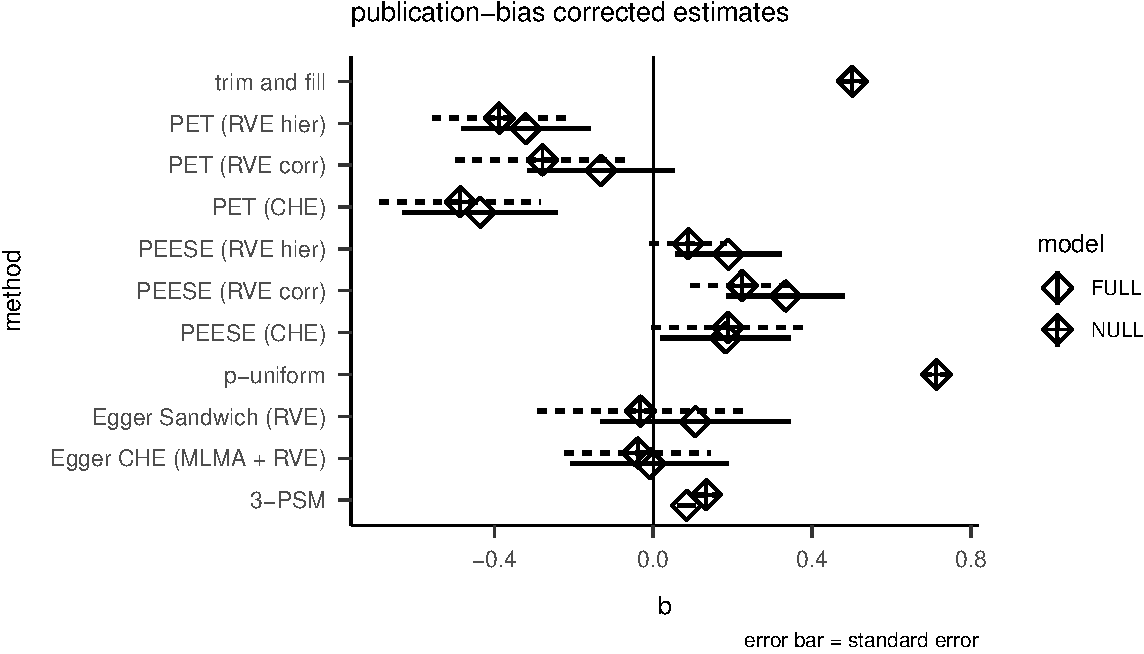
\includegraphics{MetaAnalysis_CrossSectional_files/figure-latex/pb_intercepts-1.pdf}

\begin{itemize}
\tightlist
\item
  Across all analyses, the slope (tests of small-study effect / publication bias)
  was always significant.\\
\item
  The unbiased or corrected (i.e.~publication-bias free) estimates vary tremendously
  and are thus reported as a form of a sensitivity analysis.
\end{itemize}

\hypertarget{final-words}{%
\chapter{Final Words}\label{final-words}}

We have finished a nice book.

\hypertarget{todos}{%
\chapter{TO DO's / exploratory analyses}\label{todos}}

\hypertarget{additional-subgroup-analyses-with-moderators-and-precision-estimate-to-find}{%
\section{Additional subgroup analyses with moderators and precision estimate to find}\label{additional-subgroup-analyses-with-moderators-and-precision-estimate-to-find}}

the source of heterogeneity (and small-study effect).

\hypertarget{moderator-joint-publication-group}{%
\section{Moderator Joint Publication Group}\label{moderator-joint-publication-group}}

Not sure how to do the clustering\ldots{}\\
We could parse the text and focus on surnames?\\
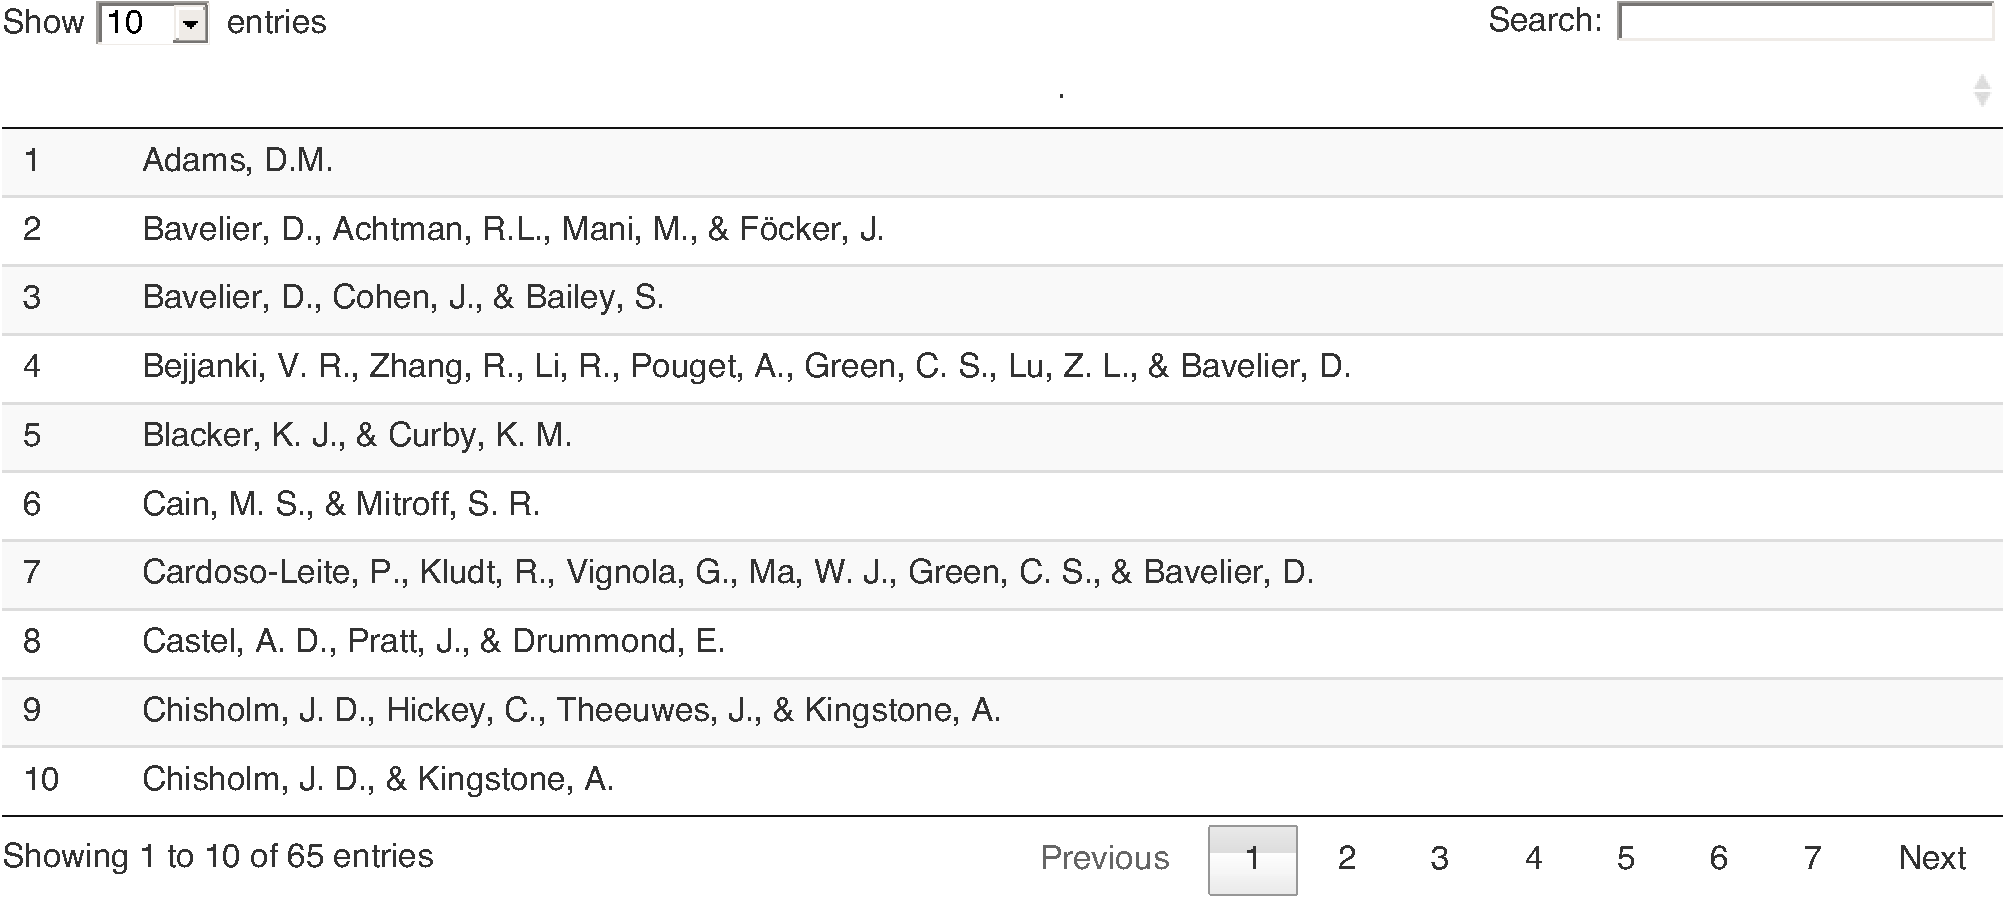
\includegraphics{MetaAnalysis_CrossSectional_files/figure-latex/unnamed-chunk-7-1.pdf}

\textbf{Cognitive sub-domains}\\
The following spatial and verbal tasks with a working-memory component will be re-coded
as measuring working memory instead of measuring spatial vs verbal skills.

\begin{tabular}{l|l|l}
\hline
Cognitive\_domain & SubDomain & examples\\
\hline
 &  & Baseline task (BAS)\\
\cline{3-3}
 &  & Perceptual Discrimination RT\\
\cline{3-3}
\multirow[t]{-3}{*}{\raggedright\arraybackslash perception} & \multirow[t]{-3}{*}{\raggedright\arraybackslash speed of processing} & Simple RT\\
\cline{1-3}
 &  & 4/8 maze task\\
\cline{3-3}
 &  & Change detection - Varying the cue-to-memory-array delay (Task 1)\\
\cline{3-3}
 &  & Change detection - Varying the test-array-to-cue delay (Task 2)\\
\cline{3-3}
 &  & Color wheel task\\
\cline{3-3}
 &  & Corsi block-tapping task (CBTT) single\\
\cline{3-3}
 &  & Enumeration\\
\cline{3-3}
 &  & Filter task\\
\cline{3-3}
 &  & N-Back (single task)\\
\cline{3-3}
\multirow[t]{-9}{*}{\raggedright\arraybackslash spatial cognition} & \multirow[t]{-9}{*}{\raggedright\arraybackslash WM} & Visual Short Term Memory (VSTM)\\
\cline{1-3}
multi-tasking & perception & UFOV dual task  / no distractors / central task\\
\cline{1-3}
 &  & Auditory 2 back - single task 2-back\\
\cline{3-3}
 &  & combiTVA\\
\cline{3-3}
 &  & N-Back\\
\cline{3-3}
 &  & N-Back (excluding the 1 back condition)\\
\cline{3-3}
 &  & OSPAN\\
\cline{3-3}
 &  & TVA whole\\
\cline{3-3}
\multirow[t]{-7}{*}{\raggedright\arraybackslash verbal cognition} & \multirow[t]{-7}{*}{\raggedright\arraybackslash WM} & Verbal Short Term Memory\\
\hline
\end{tabular}

Please, check Table \emph{List of Tasks and Cognitive Domains} to see if tasks may be missing.

\hypertarget{analysis-on-full-dataset-i.e.-without-excluding-studies-based-on-gender-ratio}{%
\section{Analysis on full dataset (i.e., without excluding studies based on gender ratio)}\label{analysis-on-full-dataset-i.e.-without-excluding-studies-based-on-gender-ratio}}

We excluded quite a large number of studies based on gender ratio.\\
Follow-up analyses will examine whether those studies that were excluded appear to have
a different ES distribution than those we kept. And I always think it's nice to anticipate
possible bad faith complaints (i.e., we excluded those studies on theoretical grounds,
because those types of gender ratios make it impossible to separate gender effects from gaming effects;
but it's nice to be able to say that if we had kept them, it wouldn't have made a difference empirically).

\hypertarget{task-difficulty}{%
\section{Task difficulty}\label{task-difficulty}}

USE mean performance (\%error, \% correct, RT) as a measure of task difficulty to check impact on ES's?

Skip to content
Search or jump to\ldots{}

Pull requests
Issues
Marketplace
Explore

\citet{bbediou}
jules32
/
bookdown-tutorial
2
11
Code
Issues
Pull requests
Actions
Projects
Wiki
Security
Insights
bookdown-tutorial/setup.Rmd
\citet{jules32}
jules32 change green to tiny
Latest commit 96f5b4a on 8 Mar 2019
History
1 contributor
66 lines (43 sloc) 2.98 KB

\hypertarget{setup}{%
\chapter{Setting up Bookdown}\label{setup}}

The \texttt{bookdown} package and \href{https://bookdown.org/yihui/bookdown/get-started.html}{book} is definitely the best way to get started. However, in practice I always find myself copying an existing, working book and modifying it instead of starting from scratch. So this tutorial is going to have you do that as well, using this book as the one you copy from.

{[}more setup here{]}

You will have to name your book's repository. To differentiate your book's repo name from this ``bookdown-tutorial'' repo, here we'll call your book ``awesome-book'' \emph{but you should consistently name it what you want to name it}.

\hypertarget{get-bookdown-tutorial-going-on-your-local-computer}{%
\section{Get ``bookdown-tutorial'' going on your local computer}\label{get-bookdown-tutorial-going-on-your-local-computer}}

\begin{enumerate}
\def\labelenumi{\arabic{enumi}.}
\tightlist
\item
  Go to \url{https://github.com/jules32/bookdown-tutorial}
\item
  Click the green ``clone or download'' button and DOWNLOAD ZIP.
\item
  Locally on your computer, unzip the folder, save it in a reasonable place
\item
  Rename 2 things from ``bookdown-tutorial'' to ``awesome-book''. You can do this in the finder/windows explorer:
\end{enumerate}

\begin{itemize}
\tightlist
\item
  the folder itself (that you just unzipped)
\item
  the .Rproj file
\end{itemize}

\begin{enumerate}
\def\labelenumi{\arabic{enumi}.}
\tightlist
\item
  Double-click the .Rproj file to launch RStudio
\item
  Install packages and restart
\end{enumerate}

\begin{itemize}
\tightlist
\item
  \texttt{install.packages("bookdown")}~\\
\item
  \texttt{install.packages("usethis")}~\\
\item
  Use the menu item Session \textgreater{} Restart R\\
\end{itemize}

\begin{enumerate}
\def\labelenumi{\arabic{enumi}.}
\tightlist
\item
  Click on the Build tab in the top right pane
\item
  Click on Build Book!
\end{enumerate}

Nice job! Now let's make it yours, and connect it to GitHub.

\hypertarget{create-your-awesome-book-github-repo}{%
\section{Create your ``awesome-book'' GitHub repo}\label{create-your-awesome-book-github-repo}}

\begin{enumerate}
\def\labelenumi{\arabic{enumi}.}
\tightlist
\item
  Go to your GitHub account: github.com/username
\item
  Click on Repositories, and the green button ``New'' to create a new repo
\item
  Name this new repo ``awesome-book''
\item
  DO NOT initialize this repo with a README
\item
  Click the green ``create repository'' button --- this will take you to your new repo
\item
  Click the tiny ``clone or download'' button near the top and COPY URL
\end{enumerate}

\hypertarget{turn-bookdown-tutorial-into-awesome-book}{%
\section{Turn ``bookdown-tutorial'' into ``awesome-book''}\label{turn-bookdown-tutorial-into-awesome-book}}

\emph{The following is from Jenny Bryan's \href{https://happygitwithr.com/existing-github-last.html}{Happy Git With R}}

\begin{enumerate}
\def\labelenumi{\arabic{enumi}.}
\tightlist
\item
  Go back to RStudio, to your ``awesome-book'' project
\item
  In the Console, type \texttt{usethis::use\_git()} and say Yes to the two prompts. This will restart R and give you a new Git tab in the upper right pane.
\item
  Now, click on the Terminal tab next to the Console tab.
\item
  Type \texttt{git\ remote\ add\ origin\ \textless{}paste\ your\ copied\ awesome-book\ github\ url\ here\textgreater{}}
\item
  Type \texttt{git\ push\ -\/-set-upstream\ origin\ master}
\end{enumerate}

\hypertarget{publish-awesome-book}{%
\section{Publish ``awesome-book''}\label{publish-awesome-book}}

Last steps!

\begin{enumerate}
\def\labelenumi{\arabic{enumi}.}
\tightlist
\item
  Go back to github.com/username/``awesome-book'' and refresh --- our files should be there! But we want it to be a book published as \url{https://username.github.io/awesome-book}.
\item
  Click Settings
\item
  Scroll down to GitHub Settings
\item
  Change the Source pulldown from ``None'' to ``master branch /docs folder''
\item
  It should say ``Your site is ready to be published at \url{https://username.github.io/awesome-book/}'' --- click the link to see!
\end{enumerate}

Now, you're set --- you just need to write your book.

\hypertarget{moving-forward}{%
\section{Moving forward}\label{moving-forward}}

As you write your .Rmd files, build the book and commit all files, including the docs/ folder, and your published book will be updated!

© 2021 GitHub, Inc.
Terms
Privacy
Security
Status
Docs
Contact GitHub
Pricing
API
Training
Blog
About
Loading complete

  \bibliography{book.bib,packages.bib}

\end{document}
